\documentclass[uplatex,dvipdfmx]{jsarticle}
\usepackage{tikz}
\usepackage{bbm}
\usepackage{amsmath,amssymb}
\usepackage{url}
\usetikzlibrary{matrix,arrows}

\newcommand{\cat}[1]{\mathbbm{#1}}
\newcommand{\arrow}{\rightarrow}
\newcommand{\functor}[3]{#1:\cat{#2}\arrow \cat{#3}}
\newcommand{\nat}[3]{#1:#2\Rightarrow #3}
\newcommand{\natf}[5]{#1:#2\Rightarrow #3:\cat{#4}\arrow \cat{#5}}
\newcommand{\tuple}[1]{\langle #1\rangle}
\newcommand{\objr}[1]{\mathrm{Obj}(#1)}
\newcommand{\obj}[1]{\mathrm{Obj}(\cat{#1})}
\newcommand{\mor}[3]{#1:#2\arrow #3}
\newcommand{\dom}{\mathrm{dom}}
\newcommand{\cod}{\mathrm{cod}}
\newcommand{\arset}[3]{\cat{#1}(#2,#3)}
\newcommand{\arsetr}[3]{#1(#2,#3)}
\newcommand{\pcobj}[1]{[#1]}
\newcommand{\funccat}[2]{\cat{#2}^\cat{#1}}
\newtheorem{proof}{証明}[section]
\newtheorem{prop}{命題}[section]
\newtheorem{define}{定義}[section]
\numberwithin{proof}{subsection}
\numberwithin{prop}{subsection}
\numberwithin{define}{subsection}
\begin{document}
	\title{圏論入門}
  \author{@otamu32}
	\maketitle
	\tableofcontents
	\section{はじめに}
	本資料は数学基礎論や計算機科学で特に使われるカルテジアン閉圏を目標に解説していく。
	また他の入門書の差別化として、できるだけ議論や具体例を圏論の中で完結するようにしている。

	\section{圏と公理}
	\begin{define}
		ある圏$\cat{C}$は以下で定義される対象集合と、任意の二対象に対する射の集合の全体、合成の演算の三つ組\[(\obj{C},\prod\limits_{A,B}^{\obj{C}}\arset{C}{A}{B},\circ)\]によって定義する。また圏は以下に示す公理を満たさなければならない。
		\begin{quote}
			\begin{description}
			\item[対象] 対象の集合$\obj{C}\ni A,B,C...$
			\item[射] 任意の対象$A,B$における射の集合$\arset{C}{A}{B}\ni f,g,h...$

			このような射の集合は任意の対象の組み合わせごとに存在する。
			また$f\in\arset{C}{A}{B}$を$\mor{f}{A}{B}$と書く。このとき$f$に対する$A$をドメイン、$B$をコドメインと呼び、射から対象への二つの演算$\dom,\cod$を用い$\dom(f)=A$、$\cod(f)=B$と表す。

			ある対象$A,B,C$、ある射$\mor{f}{A}{B}$、$\mor{g}{A}{C}$、$\mor{h}{C}{B}$について考えるとき、以下のような図式を用いて説明を行う。
			\begin{center}
				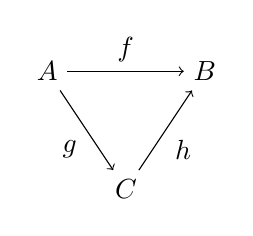
\begin{tikzpicture}[auto]
					\node (a) at (0, 0) {$A$};
					\node (b) at (2, 0) {$B$};
					\node (c) at (1, -1.5) {$C$};
					\draw[->] (a) to node {$f$}(b);
					\draw[->] (a) to node[swap] {$g$}(c);
					\draw[->] (c) to node[swap] {$h$}(b);
				\end{tikzpicture}
			\end{center}

			\item[射の合成]~\\ ある射$f,g$が$\cod(f)=\dom(g)$を満たす、つまり$\mor{f}{X}{A}$、$\mor{g}{A}{Y}$であるようなとき、合成射$\mor{g\circ f}{X}{Y}$が定まる。
			射をつなげる、という直感に反して合成射の射の順序が射の向きと逆であることに注意してほしい。

			射$h,g$の合成$h\circ g$は次のように表せる。
			また対象$A$と対象$B$の間の射は一つとは限らないので、必ずしも$h\circ g=f$が成り立つわけではない。
			\begin{center}
				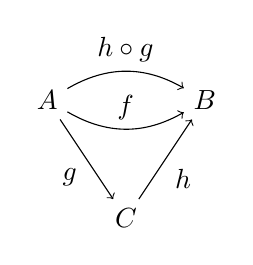
\begin{tikzpicture}[auto]
					\node (a) at (0, 0) {$A$};
					\node (b) at (2, 0) {$B$};
					\node (c) at (1, -1.5) {$C$};
					\draw[->] (a) to[bend right=30] node {$f$}(b);
					\draw[->] (a) to[bend right=-30] node {$h\circ g$}(b);
					\draw[->] (a) to node[swap] {$g$}(c);
					\draw[->] (c) to node[swap] {$h$}(b);
				\end{tikzpicture}
			\end{center}
			このような操作は任意の対象$A,B,C$における二項演算\[\mor{\circ}{\arset{\cat{C}}{B}{C}\times\arset{\cat{C}}{A}{B}}{\arset{\cat{C}}{A}{C}}\]
			で表せる。また厳密には二項演算$\circ$は任意の対象$A,B,C$の組み合わせごとに個別に存在する。
			\item[恒等射の存在] 恒等射と呼ばれる特別な射$\mor{id_A}{A}{A}$が任意の対象に存在する。
			\begin{center}
				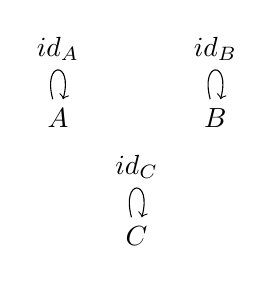
\begin{tikzpicture}[auto]
					\node (a) at (0, 0) {$A$};
					\node (b) at (2, 0) {$B$};
					\node (c) at (1, -1.5) {$C$};
					\draw[->,loop above ,looseness=10] (a) to node{$id_A$}(a);
					\draw[->,loop above ,looseness=10] (b) to node{$id_B$}(b);
					\draw[->,loop above ,looseness=10] (c) to node{$id_C$}(c);
				\end{tikzpicture}
			\end{center}
			\item[結合律] 結合則$h\circ (g\circ f)=(h\circ g)\circ f$が合成可能な任意の射$f,g,h$で成り立つ。
				\begin{center}
				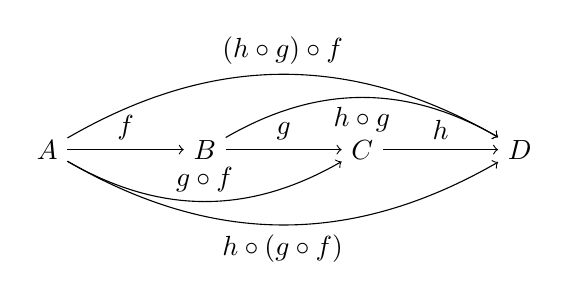
\begin{tikzpicture}[auto]
					\node (a) at (0, 0) {$A$};
					\node (b) at (2, 0) {$B$};
					\node (c) at (4, 0) {$C$};
					\node (d) at (6, 0) {$D$};
					\draw[->] (a) to node {$f$}(b);
					\draw[->] (b) to node {$g$}(c);
					\draw[->] (c) to node {$h$}(d);
					\draw[->] (a) to[bend right=30] node {$g\circ f$}(c);
					\draw[->] (a) to[bend right=30] node[swap] {$h\circ(g\circ f)$}(d);
					\draw[->] (b) to[bend left=30] node[swap] {$h\circ g$}(d);
					\draw[->] (a) to[bend left=30] node {$(h\circ g)\circ f$}(d);
				\end{tikzpicture}
			\end{center}
			\item[単位元律]~\\ 任意の対象$A$と対応する恒等射$\mor{id_A}{A}{A}$、任意の射$\mor{f}{X}{A}$、$\mor{g}{A}{Y}$において\[id_A\circ f=f,\ g\circ id_A=g\]が成り立つ。

			恒等射をある射に合成しても、合成する前の射と等しくなることから、直感的に恒等射は何も行わない射のように考えられる。

			\begin{center}
				\begin{tikzpicture}[auto]
					\node (x) at (0, 0) {$X$};
					\node (a) at (2, 0) {$A$};
					\node (y) at (4, 0) {$Y$};
					\draw[->] (x) to node {$f$}(a);
					\draw[->,loop above, looseness=20] (a) to node {$id_A$}(a);
					\draw[->] (a) to node {$g$}(y);
				\end{tikzpicture}
				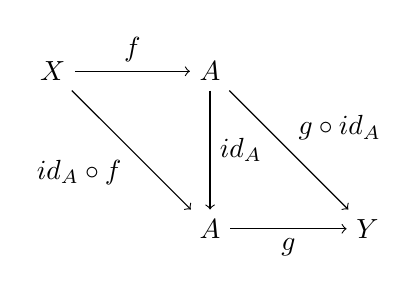
\begin{tikzpicture}[auto]
					\node (a) at (0, 0) {$X$};
					\node (b) at (2, 0) {$A$};
					\node (b') at (2, -2) {$A$};
					\node (c) at (4, -2) {$Y$};
					\draw[->] (a) to node {$f$}(b);
					\draw[->] (b) to node {$id_A$}(b');
					\draw[->] (b') to node[swap]  {$g$}(c);
					\draw[->] (a) to node[swap]  {$id_A\circ f$}(b');
					\draw[->] (b) to node {$g\circ id_A$}(c);
				\end{tikzpicture}
			\end{center}
		\end{description}
			\end{quote}
	\end{define}
	\begin{define}[圏の同一性]
		圏$\cat{A,B}$が同一、$\cat{A}=\cat{B}$であるとは、対象の集合、射の集合、合成の演算が集合、写像として等しいということである。
		
		同様に対象や射の同一性も対象の集合の元、射の集合の元の等しさで表される。
	\end{define}
	次に圏の例として集合の圏を挙げる。
	\begin{define}[集合の圏]
		圏$\cat{Set}$を以下の要素から構成する。
		\begin{quote}
			\begin{description}
				\item[対象] $\obj{Set}$を小さな集合の集合とする。

				「小さい」は自己言及を避けるための条件であり、実際に$\obj{Set}$は大きい集合となるため$\obj{Set}$には含まれない。
				\item[射] 二対象$A,B$に対する射集合$\arset{Set}{A}{B}$を小さな集合$A$から小さな集合$B$への写像の集合$\arset{Set}{A}{B}$とする。

				また紛らわしい場合を除いて小さい集合を集合と呼ぶことにする。

				集合の圏では一般的な圏とは違い、対象を集合として元をとることができる。
				そして同対象間に射が二つあったとき、二つの写像が等しいかどうかを元の対応関係で確かめることができる。
				つまり、二つの写像$\mor{f,g}{A}{B}$と集合$A$の任意の元$a$に対して、\[f(a)=g(a)\]ならば$f=g$が成り立つ、ということである。以降は元の対応関係を用いて集合の圏の射である写像を定義していく。

				\item[射の合成]  二つの写像$\mor{f}{A}{B}$、$\mor{g}{B}{C}$の合成写像$\mor{g\circ f}{A}{C}$を$A$の任意の元$a$に対して\[(g\circ f)(a)=g(f(a))\]となるように定義する。

				集合の圏は一般的な圏とは違い、元の対応関係を調べるだけで射が等しくなることを示せる。
				\item[恒等射の存在] 任意の集合$A$に対する恒等射$id_A$を$A$の任意の元$a$に対して\[id_A(a)=a\]となるように定義する。
				\item[結合律] 任意の写像$\mor{f}{A}{B}$、$\mor{g}{B}{C}$、$\mor{h}{C}{D}$に対して$h\circ(g\circ f)=(h\circ g)\circ f$が成り立つことを示せばよい。
				それぞれ合成写像の定義を用いて
				\begin{align*}
					((h\circ g)\circ f)(a)&=(h\circ g)(f(a))\\
					&=h(g(f(a)))\\
					&=h((g\circ f)(a))\\
					&=(h\circ(g\circ f))(a)
				\end{align*}
				となり、写像の合成では結合律が成り立つ。
				\item[単位元律] 任意の集合$A$と対応する恒等写像$id_A$、任意の写像$\mor{f}{X}{A}$、$\mor{g}{A}{Y}$において\[(id_A\circ f)(x)=f(x),\ (g\circ id_A)(a)=g(a)\]が成り立つことを示せばよい。
				\begin{align*}
					(id_A\circ f)(x)&=id_A(f(x))&\text{(写像の合成の定義)}\\
					&=f(x)&\text{{(恒等写像の定義)}}\\
					(g\circ id_A)(a)&=g(id_A(a))&\text{(写像の合成の定義)}\\
					&=g(a)&\text{{(恒等写像の定義)}}
				\end{align*}
				よって単位元律が成り立つ。
			\end{description}
		\end{quote}
	\end{define}
	
	集合の圏の射である写像は、任意の元が同じ元に対応することによって射が等しいことを示せたが、一般の圏ではそうは限らない。そもそも対象の元を取ることができるとは限らないし、元の対応関係が一致していても同じ射であるとも限らない。

	集合の圏を集合によって定義したが以降で使用する集合としての性質は、元の対応関係により射が等しいことを示せること以外はほとんど使用しない。仮に使用したとしても、直ちに圏論的な定義に置き換える。
	\section{圏論の基本概念}
	圏論では対象の性質をその対象をドメイン、コドメインとする射の性質によって与える。
	直感的にはある対象を述べる場合、「どのように構成されるか」ではなく「どのように振舞うか」で述べるように思える。

	まずはこれまで図示してきた図式について数学的な定義を与える。
	\begin{define}[図式(部分圏)]
		ある圏$\cat{C}$のある図式(部分圏)とは、圏$\cat{C}$に含まれるいくつかの対象と、いくつかの射で構成される圏であり、任意の対象に対応する恒等射を含み、図式中の任意の合成可能な二射$\mor{f}{X}{Y},\mor{g}{Y}{Z}$が含まれるとき、その合成射$g\circ f$も含むような圏である。
	\end{define}
	また図式は単に図示するために使用する以外にも、圏論のいくつかの概念を定義するのにも用いられる。
	\begin{define}[可換]
		圏におけるいくつかの射と対象の集まりである図式が可換である。すなわち可換図式であるとは、図式中の対象を頂点、図式中の射を辺とする有向グラフを考えたとき、任意の頂点$C,C'$において$C$から$C'$への任意の経路によって表される射が等しいときである。
	\end{define}
	例えば以下の図式において$j\circ g=l\circ i,k\circ h=m\circ j,k\circ h\circ g=m\circ j\circ g = m\circ l\circ i$が成り立つとすると、これは可換図式になる。

	\begin{center}
		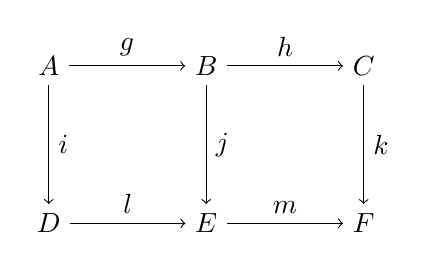
\begin{tikzpicture}[auto]
			\node (a) at (0, 0) {$A$};
			\node (b) at (2, 0) {$B$};
			\node (c) at (4, 0) {$C$};
			\node (d) at (0, -2) {$D$};
			\node (e) at (2, -2) {$E$};
			\node (f) at (4, -2) {$F$};
			\draw[->] (a) to node {$g$}(b);
			\draw[->] (b) to node {$h$}(c);
			\draw[->] (a) to node {$i$}(d);
			\draw[->] (b) to node {$j$}(e);
			\draw[->] (c) to node {$k$}(f);
			\draw[->] (d) to node {$l$}(e);
			\draw[->] (e) to node {$m$}(f);
		\end{tikzpicture}
	\end{center}

	\subsection{元}
		集合の圏では集合から集合への関数の性質を述べるのに集合の元を用いることができるが、圏の対象では一般的に元を取ることができない。
		しかしある圏$\cat{C}$に終対象$1$と呼ばれる特別な対象が存在するとき、$\cat{C}$の任意の対象$A$のある元(global elements)はある射$\mor{a}{1}{A}$で表せる。
		\begin{center}
			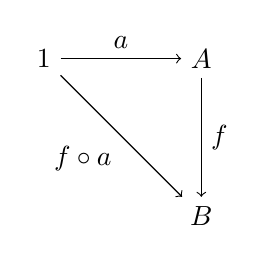
\begin{tikzpicture}[auto]
				\node (a) at (2, 0) {$A$};
				\node (b) at (2, -2) {$B$};
				\node (1) at (0, 0) {$1$};
				\draw[->] (1) to node {$a$}(a);
				\draw[->] (1) to node[swap] {$f\circ a$}(b);
				\draw[->] (a) to node {$f$}(b);
			\end{tikzpicture}
		\end{center}

		射$\mor{f}{A}{B}$に対して$\mor{a}{1}{A}$を適用する操作は、そのまま関数の合成$\mor{f\circ a}{1}{B}$で表せる。
		また射を適用した元もまた終対象からの射になるから$f\circ a$もまた対象$B$の元になる。

		後に詳しく説明するが、要素をただ一つ持つような集合は集合の圏における終対象$1$であり、$1$から集合$A$への写像である元は実際に集合$A$の元とみなせる。
		\begin{prop}[集合の圏における元]
			集合の圏には終対象となる集合$1$が存在し、任意の集合$A$において元$\mor{a}{1}{A}$は集合における元に対し一意に対応する。
		\end{prop}
	\subsection{同型}
	圏論では射の等しさを表すときには等号を使うが、対象に対しての等号は制約が多い。そのため同型と呼ばれる同値関係を代わりに用いる。
	\begin{define}[同型]
		ある対象$A$と$B$が同型、つまり$A\cong B$であるとは、$i\circ i^{-1}=id_B$と$i^{-1}\circ i=id_A$を満たすようなある二つの射$\mor{i}{A}{B}$とその逆射$\mor{i^{-1}}{B}{A}$が存在するときである。
		また、このような射$i,i^{-1}$を同型射と呼ぶ。
	\end{define}
	\begin{center}
		\begin{tikzpicture}[auto]
			\node (a) at (-4, -1) {$A$};
			\node (b) at (-2, -1) {$B$};
			\draw[->,transform canvas={yshift=-3pt}] (a) to node[swap] {$i$}(b);
			\draw[->,transform canvas={yshift=3pt}] (b) to node[swap] {$i^{-1}$}(a);

			\node (a) at (0, 0) {$A$};
			\node (b) at (2, 0) {$B$};
			\node (b') at (0, -2) {$B$};
			\draw[->] (a) to node[swap] {$i$}(b');
			\draw[->] (b) to node {$id_B$}(b');
			\draw[->] (b) to node[swap] {$i^{-1}$}(a);

			\node (a) at (4, 0) {$B$};
			\node (b) at (6, 0) {$A$};
			\node (b') at (4, -2) {$A$};
			\draw[->] (a) to node[swap] {$i^{-1}$}(b');
			\draw[->] (b) to node {$id_A$}(b');
			\draw[->] (b) to node[swap] {$i$}(a);
		\end{tikzpicture}
	\end{center}
	同型は対象同士の相互互換のような関係性を表しているように思える。

  \begin{proof}
    同型が同値関係であることを証明する。
    \begin{quote}
			\begin{description}
				\item[反射律] 任意の対象$A$で$A\cong A$が成り立つことを証明すれば良い。$\mor{id_A}{A}{A}$を同型射とその逆射$(id_A)^{-1}$をまた$id_A$とすると、\[id_A\circ id_A = id_A,\,id_A\circ id_A = id_A\]が成り立つから、$id_A$は同型射であり$A\cong A$である。

				\item[対称律] 同型$A\cong B\Longrightarrow B\cong A$を示せば良い。同型$A\cong B$が同型射$\mor{i}{A}{B}$とその逆射$\mor{i^{-1}}{B}{A}$によって成り立つとする。この時、$i^{-1}$の逆射を$i$とみなすと、$i^{-1}\circ i=id_A$と$i\circ i^{-1}=id_B$が成り立つから、$B\cong A$となる。
				\item[推移律] $A\cong B,B\cong C\Longrightarrow A\cong C$を示せば良い。$A\cong B$の同型射を$\mor{i}{A}{B}$、$\mor{i^{-1}}{B}{A}$、$B\cong C$の同型射を$\mor{j}{B}{C}$、$\mor{j^{-1}}{C}{B}$とする。この時、$j\circ i$と$i^{-1}\circ j^{-1}$が同型射になることを示せば良い。
        \begin{center}
          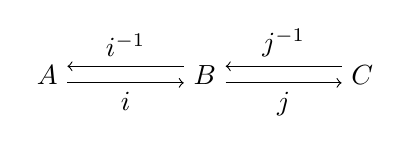
\begin{tikzpicture}[auto]
            \node (a) at (0, 0) {$A$};
            \node (b) at (2, 0) {$B$};
            \node (c) at (4, 0) {$C$};
            \draw[->,transform canvas={yshift=-3pt}] (a) to node[swap] {$i$}(b);
            \draw[->,transform canvas={yshift=3pt}] (b) to node[swap] {$i^{-1}$}(a);

            \draw[->,transform canvas={yshift=-3pt}] (b) to node[swap] {$j$}(c);
            \draw[->,transform canvas={yshift=3pt}] (c) to node[swap] {$j^{-1}$}(b);
          \end{tikzpicture}
        \end{center} 
				\begin{align*}
          (j\circ i)\circ (i^{-1}\circ j^{-1})&=j\circ(i\circ i^{-1})\circ j^{-1}&\text{(結合則)}\\
          &=j\circ(id_B)\circ j^{-1}&\text{(同型射の定義)}\\
          &=j\circ j^{-1}&\text{(恒等射の性質)}\\
          &=id_C&\text{(同型射の定義)}\\
          (i^{-1}\circ j^{-1})\circ(j\circ i)&=i^{-1}\circ(j^{-1}\circ j)\circ i&\text{(結合則)}\\
          &=i^{-1}\circ(id_B)\circ i&\text{(同型射の定義)}\\
          &=i^{-1}\circ i&\text{(恒等射の性質)}\\
          &=id_A&\text{(同型射の定義)}\\
        \end{align*}
        よって$j\circ i$と$i^{-1}\circ j^{-1}$は同型射となり、$A\cong C$が成り立つ。
      \end{description}
    \end{quote}
  \end{proof}


	\begin{prop}[集合の圏の同型]
		集合の圏$\cat{Set}$において、同型$A\cong B$$\Longleftrightarrow$同型射$\mor{i}{A}{B}$が全単射。

		また全単射は、任意の元$\mor{b}{1}{B}$に対して、$i(a)=b$が成り立つようなある元$\mor{a}{1}{A}$が一意に存在することであり、この対応を一対一対応と呼ぶ。
	\end{prop}

	\begin{proof}
		$(\Longleftarrow)$だけ証明する。


		まずは$b$に対する等式を満たすような$a$が存在することを示す
		任意の元$\mor{b}{1}{B}$に対応する元$\mor{a}{1}{A}$を$a=i^{-1}(b)$とする。すると
		\begin{align*}
			i(a)&=i(i^{-1}(b))&\text{(元$a$の定義)}\\
			&=(i\circ i^{-1})(b)&\text{(写像の合成の定義)}\\
			&=b&\text{(同型射の定義)}\\
		\end{align*}
		\[i(a)=i(i^{-1}(b))=i\circ i^{-1}(b)=b\]となり、確かにこのような$a$は存在する。

		$b$に対する元$a$の一意性を示すには、任意の元$\mor{a'}{1}{A}$において$i(a)=b,\ i(a')=b$ならば$a=a'$を示せばよい。

		$i(a')=b$と仮定すると、
		\begin{align*}
			a&=i^{-1}(b)&\text{(元$a$の定義)}\\
			&=i^{-1}(i(a'))&\text{(仮定)}\\
			&=(i^{-1}\circ i)(a')&\text{(写像の合成の定義)}\\
			&=a'&\text{(同型射の定義)}
		\end{align*}
		よって$b$に対する$i(a)=b$を満たすような$a$が一意に存在することが示せたので、$i$が全単射であることが示せた。
	\end{proof}

	\section{普遍性}
	普遍性はある対象と射を特徴づけるために使用され、ある図式を可換にするような射が一意に存在する。というように記述され、図式中の射と一意に定まる射の対応関係を示すことが多い。このような議論は集合の圏における同型でも扱ったが、実際に以下で紹介する普遍性は集合の全単射で表せる。詳しくは別の章で説明する。
	\subsection{積}
	\begin{define}[積]
		対象$A$と$B$が積を持つとは、以下の条件を満たす組$(A\times B,\pi_{L,A\times B},\pi_{R,A\times B})$が存在するときである。
		\begin{quote}
			\begin{description}
			\item[積対象と射影射]ある積対象$A\times B$とある二つの射$\mor{\pi_{L,A\times B}}{A\times B}{A}$、$\mor{\pi_{R,A\times B}}{A\times B}{B}$が存在する。
			この時、積対象と射影射の組$(A\times B,\pi_{L,A\times B},\pi_{R,A\times B})$を$A,B$の積と呼ぶ。


			\begin{center}
				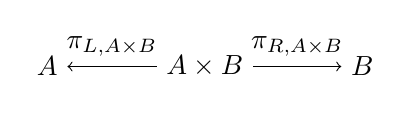
\begin{tikzpicture}[auto]
					\node (a) at (0, 0) {$A$};
					\node (b) at (4, 0) {$B$};
					\node (ab) at (2, 0) {$A\times B$};
					\draw[->] (ab) to node[swap] {$\pi_{L,A\times B}$}(a);
					\draw[->] (ab) to node {$\pi_{R,A\times B}$}(b);
				\end{tikzpicture}
			\end{center}
			また$(A\times A,\pi_{L,A\times B},\pi_{R,A\times B})$などの紛らわしい場合を除いて$\pi_{L,A\times B}$を$\pi_A$、$\pi_{R,A\times B}$を$\pi_B$と表記する。
			\item[任意の対象からの射]任意の対象$X$に対し任意の二射$\mor{f}{X}{A}$、$\mor{g}{X}{B}$が存在するとする。
			\begin{center}
				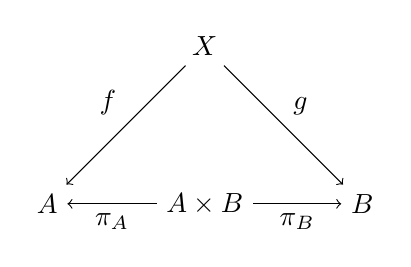
\begin{tikzpicture}[auto]
					\node (a) at (0, 0) {$A$};
					\node (b) at (4, 0) {$B$};
					\node (ab) at (2, 0) {$A\times B$};
					\node (x) at (2, 2) {$X$};
					\draw[->] (ab) to node {$\pi_A$}(a);
					\draw[->] (ab) to node[swap] {$\pi_B$}(b);
					\draw[->] (x) to node[swap] {$f$}(a);
					\draw[->] (x) to node {$g$}(b);
				\end{tikzpicture}
			\end{center}
			\item[普遍性]任意の二射$f,g$に対して図式を可換にする、つまり$\pi_A\circ\tuple{f,g}=f$、$\pi_B\circ\tuple{f,g}=g$が成り立つような射$\tuple{f,g}$を射の対とする。

			またこのような射の対$\tuple{f,g}$は任意の二射$f,g$に対して一意に存在する。

			射の対は一意に存在するが、ある射$h$が二射$f,g$に対する射の対である条件に一意性と存在性は含まれない。射の対であることを示すには単に二つの等式$\pi_A\circ h=f$、$\pi_B\circ h=g$が成り立つことを確認するだけでよい。

			\begin{center}
				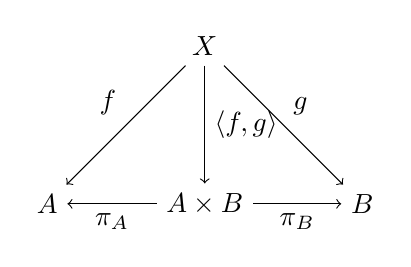
\begin{tikzpicture}[auto]
					\node (a) at (0, 0) {$A$};
					\node (b) at (4, 0) {$B$};
					\node (ab) at (2, 0) {$A\times B$};
					\node (x) at (2, 2) {$X$};
					\draw[->] (ab) to node {$\pi_A$}(a);
					\draw[->] (ab) to node[swap] {$\pi_B$}(b);
					\draw[->] (x) to node[swap] {$f$}(a);
					\draw[->] (x) to node {$g$}(b);
					\draw[->] (x) to node {$\tuple{f,g}$}(ab);
				\end{tikzpicture}
			\end{center}
			\end{description}
		\end{quote}

	\end{define}

	射の対が一意であるとは、射の対$\tuple{f,g}$に対し、ある射$\mor{h}{X}{A\times B}$が存在して$\pi_A\circ h=f$、$\pi_B\circ h=g$を満たすとき、$h=\tuple{f,g}$となることである。


	また、図式を可換にする射の対$\tuple{f,g}$の存在性は任意の射の組み合わせに対して射の対が存在することを示し、一意性は射の対が含んでいる二つの射以外の判別可能な要素を含みようがないことを示している。

	\begin{define}[積を持つ圏]
		すべての圏、すべての二対象に対して積が存在するとは限らないが、ある圏$\cat{C}$の任意の二対象に対して積が存在するとき、圏$\cat{C}$は積を持つという。
	\end{define}
	ここで$X$に終対象$1$を当てはめると、元$\mor{a}{1}{A}$、元$\mor{b}{1}{B}$に対して$\pi_A\circ\tuple{a,b}=a$、$\pi_B\circ\tuple{a,b}=b$が成り立つような$\tuple{a,b}$が一意に存在することがわかる。
	\begin{center}
		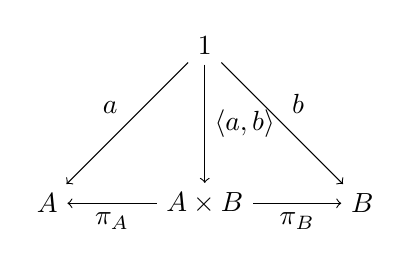
\begin{tikzpicture}[auto]
			\node (a) at (0, 0) {$A$};
			\node (b) at (4, 0) {$B$};
			\node (ab) at (2, 0) {$A\times B$};
			\node (x) at (2, 2) {$1$};
			\draw[->] (ab) to node {$\pi_A$}(a);
			\draw[->] (ab) to node[swap] {$\pi_B$}(b);
			\draw[->] (x) to node[swap] {$a$}(a);
			\draw[->] (x) to node {$b$}(b);
			\draw[->] (x) to node {$\tuple{a,b}$}(ab);
		\end{tikzpicture}
	\end{center}

	次に積の性質をいくつか見ていく。
	\begin{prop}[射の対の分配則]
		$\mor{f}{X}{A}$、$\mor{g}{X}{B}$、$\mor{h}{Y}{X}$に対して\[\tuple{f,g}\circ h=\tuple{f\circ h,g\circ h}\]が成り立つ
	\end{prop}
	\begin{proof}
		積$A\times B$に対し、$\mor{f\circ h}{Y}{A}$、$\mor{g\circ h}{Y}{B}$の射の対$\mor{\tuple{f\circ h,g\circ h}}{Y}{A\times B}$を考える。

		これは$\mor{\tuple{f,g}\circ h}{Y}{A\times B}$が二射$f\circ h,g\circ h$における射の対となることを示し、射の対の一意性から証明すればよい。

		積の普遍性より、
		\begin{align*}
			\pi_A\circ\tuple{f\circ h,g\circ h}&=f\circ h\\
			\pi_B\circ\tuple{f\circ h,g\circ h}&=g\circ h
		\end{align*}
		が成り立つような射$\tuple{f\circ h,g\circ h}$は一意に存在する。

		また、
		\begin{align*}
			\pi_A\circ(\tuple{f,g}\circ h)&=(\pi_A\circ\tuple{f,g})\circ h&\text{(結合則)}\\
			&=f\circ h&\text{(射の対の可換性)}\\
			\pi_B\circ(\tuple{f,g}\circ h)&=(\pi_B\circ\tuple{f,g})\circ h&\text{(結合則)}\\
			&=g\circ h&\text{(射の対の可換性)}
		\end{align*}
		$\pi_A\circ(\tuple{f,g}\circ h)=f\circ h$、$\pi_B\circ(\tuple{f,g}\circ h)=g\circ h$となるため、$\mor{\tuple{f,g}\circ h}{Y}{A\times B}$も同様に二射$f\circ h,g\circ h$の射の対になる。
		よって射の対の一意性より、$\tuple{f,g}\circ h=\tuple{f\circ h,g\circ h}$が成り立つ。
	\end{proof}

	\begin{center}
		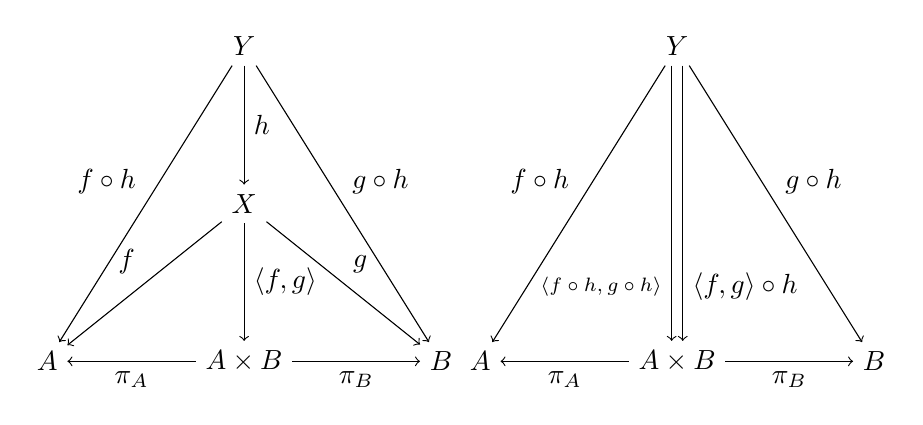
\begin{tikzpicture}[auto]
			\node (y) at (3, 4) {$Y$};
			\node (a) at (0.5, 0) {$A$};
			\node (b) at (5.5, 0) {$B$};
			\node (ab) at (3, 0) {$A\times B$};
			\node (x) at (3, 2) {$X$};
			\draw[->] (y) to node {$h$}(x);
			\draw[->] (y) to node[swap] {$f\circ h$}(a);
			\draw[->] (y) to node {$g\circ h$}(b);
			\draw[->] (ab) to node {$\pi_A$}(a);
			\draw[->] (ab) to node[swap] {$\pi_B$}(b);
			\draw[->] (x) to node[swap] {$f$}(a);
			\draw[->] (x) to node {$g$}(b);
			\draw[->] (x) to node {$\tuple{f,g}$}(ab);

			\node (y) at (8.5, 4) {$Y$};
			\node (a) at (6, 0) {$A$};
			\node (b) at (11, 0) {$B$};
			\node (ab) at (8.5, 0) {$A\times B$};
			\draw[->, transform canvas={xshift=2pt}] (y) to node[yshift=-30pt] {$\tuple{f,g}\circ h$}(ab);
			\draw[->, transform canvas={xshift=-2pt}] (y) to node[yshift=-30pt, swap] {\scriptsize{$\tuple{f\circ h,g\circ h}$}}(ab);
			\draw[->] (y) to node[swap] {$f\circ h$}(a);
			\draw[->] (y) to node {$g\circ h$}(b);
			\draw[->] (ab) to node {$\pi_A$}(a);
			\draw[->] (ab) to node[swap] {$\pi_B$}(b);
		\end{tikzpicture}
	\end{center}

  普遍性を用いた基本的な等式の証明はこのように、等式の右辺左辺が同じ二射の射の対になるような図式を考え、射の対の一意性から等式を示す。
  この証明では積の図式に対象$Y$と射$h$をつなげて拡張することで、新しい積の図式を考えた。

	また$Y$に終対象$1$、$h$に元$\mor{x}{1}{X}$を当てはめると、同様に$\tuple{f,g}\circ x=\tuple{f\circ x,g\circ x}$となる。
	つまり射の対は与えられた元にそれぞれの射を適用し、また対を取るような射だと考えられる。
	\begin{center}
		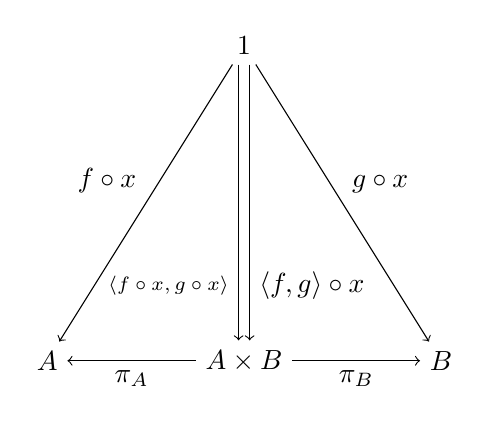
\begin{tikzpicture}[auto]
			\node (y) at (8.5, 4) {$1$};
			\node (a) at (6, 0) {$A$};
			\node (b) at (11, 0) {$B$};
			\node (ab) at (8.5, 0) {$A\times B$};
			\draw[->, transform canvas={xshift=2pt}] (y) to node[yshift=-30pt] {$\tuple{f,g}\circ x$}(ab);
			\draw[->, transform canvas={xshift=-2pt}] (y) to node[yshift=-30pt, swap] {\scriptsize{$\tuple{f\circ x,g\circ x}$}}(ab);
			\draw[->] (y) to node[swap] {$f\circ x$}(a);
			\draw[->] (y) to node {$g\circ x$}(b);
			\draw[->] (ab) to node {$\pi_A$}(a);
			\draw[->] (ab) to node[swap] {$\pi_B$}(b);
		\end{tikzpicture}
	\end{center}

	次に、任意の積から任意の積への射である、射の積を定義していく。
	\begin{define}[射の積]
		射$\mor{f}{A}{A'}$、$\mor{g}{B}{B'}$に対して射の積$\mor{f\times g}{A\times B}{A'\times B'}$を\[f\times g = \tuple{f\circ\pi_A,g\circ\pi_B}\]と定義する。
		\begin{center}
			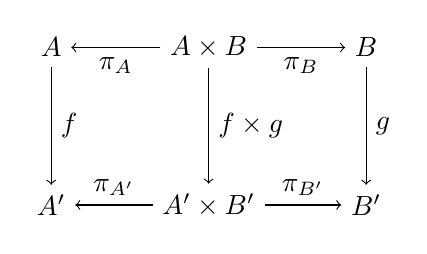
\begin{tikzpicture}[auto]
				\node (a) at (0, 0) {$A$};
				\node (ab) at (2, 0) {$A\times B$};
				\node (b) at (4, 0) {$B$};
				\node (a') at (0, -2) {$A'$};
				\node (a'b') at (2, -2) {$A'\times B'$};
				\node (b') at (4, -2) {$B'$};
				\draw[->] (a'b') to node[swap] {$\pi_{A'}$}(a');
				\draw[->] (a'b') to node {$\pi_{B'}$}(b');
				\draw[->] (ab) to node {$\pi_A$}(a);
				\draw[->] (ab) to node[swap] {$\pi_B$}(b);
				\draw[->] (a) to node {$f$}(a');
				\draw[->] (b) to node {$g$}(b');
				\draw[->] (ab) to node {$f\times g$}(a'b');
			\end{tikzpicture}
		\end{center}
	\end{define}
	射の対は任意の対象から任意の積への射であるのに対し、射の積は任意の積から任意の積への射である。
	二つの対象から二つの対象へ射を一つの射に纏めることから、直感的に射の積は並列処理のように思える。

	\begin{prop}[積と合成の交換]
		射の積$\mor{f\times g}{A\times B}{A'\times B'}$、$\mor{f'\times g'}{A'\times B'}{A''\times B''}$に対して、\[(f'\times g')\circ(f\times g)=(f'\circ f)\times(g'\circ g)\]が成り立つ。
	\end{prop}
	\begin{proof}
		積$(A''\times B'',\pi_{A''},\pi_{B''})$において対$(X,f,g)$に$(A\times B,f'\circ f\circ\pi_A$,$g'\circ g\circ\pi_B)$を当てはめると射$\mor{\tuple{f'\circ f\circ\pi_A,g'\circ g\circ\pi_B}}{A\times B}{A''\times B''}$が得られる。また射の積の定義より\[\tuple{f'\circ f\circ\pi_A,g'\circ g\circ\pi_B}=(f'\circ f)\times(g'\circ g)\]が成り立つ。
		次に$(f'\times g')\circ(f\times g)$も同様に$(A\times B,f'\circ f\circ\pi_A$,$g'\circ g\circ\pi_B)$に対する射の対であることを示す。
		\begin{align*}
			\pi_{A''}\circ(f'\times g')\circ(f\times g)&=\pi_{A''}\circ\tuple{f'\circ\pi_A,g'\circ\pi_B}\circ\tuple{f\circ\pi_A,g\circ\pi_B}&\text{(射の積の定義)}\\
			&=f'\circ\pi_{A'}\circ\tuple{f\circ\pi_A,g\circ\pi_B}&\text{(射の対の可換性)}\\
			&=f'\circ f\circ\pi_A&\text{(射の対の可換性)}\\
			\pi_B\circ(f'\times g')\circ(f\times g)&=\pi_{B''}\circ\tuple{f'\circ\pi_A,g'\circ\pi_B}\circ\tuple{f\circ\pi_A,g\circ\pi_B}&\text{(射の積の定義)}\\
			&=g'\circ\pi_{B'}\circ\tuple{f\circ\pi_A,g\circ\pi_B}&\text{(射の対の可換性)}\\
			&=g'\circ g\circ\pi_B&\text{(射の対の可換性)}
		\end{align*}
	\begin{center}
		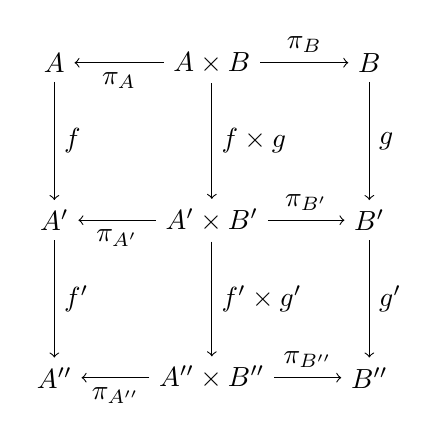
\begin{tikzpicture}[auto]
			\node (a) at (0, 0) {$A$};
			\node (a') at (0, -2) {$A'$};
			\node (a'') at (0, -4) {$A''$};
			\node (ab) at (2, 0) {$A\times B$};
			\node (ab') at (2, -2) {$A'\times B'$};
			\node (ab'') at (2, -4) {$A''\times B''$};
			\node (b) at (4, 0) {$B$};
			\node (b') at (4, -2) {$B'$};
			\node (b'') at (4, -4) {$B''$};
			\draw[->] (ab) to node{$\pi_{A}$}(a);
			\draw[->] (ab) to node{$\pi_{B}$}(b);
			\draw[->] (ab') to node{$\pi_{A'}$}(a');
			\draw[->] (ab') to node{$\pi_{B'}$}(b');
			\draw[->] (ab'') to node{$\pi_{A''}$}(a'');
			\draw[->] (ab'') to node{$\pi_{B''}$}(b'');
			\draw[->] (a) to node{$f$}(a');
			\draw[->] (a') to node{$f'$}(a'');
			\draw[->] (b) to node{$g$}(b');
			\draw[->] (b') to node{$g'$}(b'');
			\draw[->] (ab) to node{$f\times g$}(ab');
			\draw[->] (ab') to node{$f'\times g'$}(ab'');
		\end{tikzpicture}
		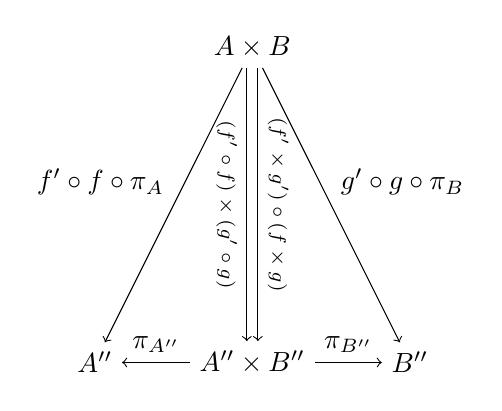
\begin{tikzpicture}[auto]
			\node (a'') at (0, -4) {$A''$};
			\node (ab) at (2, 0) {$A\times B$};
			\node (ab'') at (2, -4) {$A''\times B''$};
			\node (b'') at (4, -4) {$B''$};
			\draw[->] (ab) to node[swap]{$f'\circ f\circ\pi_A$}(a'');
			\draw[->] (ab) to node{$g'\circ g\circ\pi_B$}(b'');
			\draw[->] (ab'') to node[swap]{$\pi_{A''}$}(a'');
			\draw[->] (ab'') to node{$\pi_{B''}$}(b'');
			\draw[->,transform canvas={xshift=2pt}] (ab) to node[sloped]{\scriptsize{$(f'\times g')\circ(f\times g)$}} (ab'');
			\draw[->,transform canvas={xshift=-2pt}] (ab) to node[sloped,swap]{\scriptsize{$(f'\circ f)\times(g'\circ g)$}}(ab'');
		\end{tikzpicture}
	\end{center}

		\[\pi_A\circ(f'\times g')\circ(f\times g)=f'\circ f\circ\pi_A,\ \pi_B\circ(f'\times g')\circ(f\times g)=g'\circ g\circ\pi_B\]の二式が成り立つから、$(f'\times g')\circ(f\times g)$も同様に$(A\times B,f'\circ f\circ\pi_A$,$g'\circ g\circ\pi_B)$に対する射の対である。

		よって$(f'\times g')\circ(f\times g)=(f'\circ f)\times(g'\circ g)$が成り立つ。
	\end{proof}
	射の積を並列での合成とみなすならば、射の合成は直列での合成を表し、積と合成の交換はどちらの合成を先に計算しても結果が変わらないことを表す。
	\begin{prop}[射影射の対]
		ある積$(A\times B,\pi_A,\pi_B)$に対して$\tuple{\pi_A,\pi_B}=id_{A\times B}$が成り立つ。
	\end{prop}
	\begin{proof}
		積$(A\times B,\pi_A,\pi_B)$に対して二射$\pi_A,\pi_B$の射の対$\mor{\tuple{\pi_A,\pi_B}}{A\times B}{A\times B}$を考える。この時、$\mor{id_{A\times B}}{A\times B}{A\times B}$も同様に二射$\pi_A,\pi_B$の射の対であることを示せばよい。


		$\pi_{A}\circ id_{A\times B}=\pi_{A}$と$\pi_{B}\circ id_{A\times B}=\pi_{B}$が成り立つから、$id_{A\times B}$は$\pi_A$と$\pi_B$の射の対になる。よって射の対の一意性より、$\tuple{\pi_A,\pi_B}=id_{A\times B}$が成り立つ。
		\begin{center}
			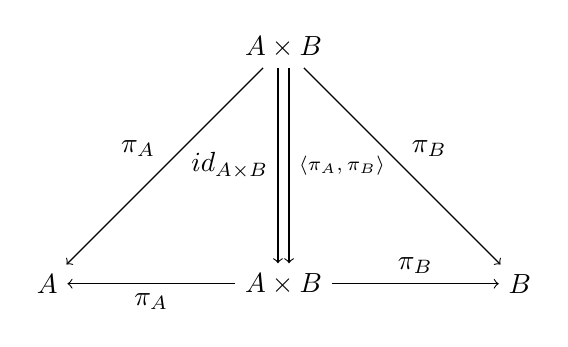
\begin{tikzpicture}[auto]
				\node (a) at (0, 0) {$A$};
				\node (ab) at (3, 0) {$A\times B$};
				\node (b) at (6, 0) {$B$};
				\node (p) at (3, 3) {$A\times B$};
				\draw[->] (p) to node[swap]{$\pi_A$}(a);
				\draw[->] (p) to node{$\pi_B$}(b);
				\draw[->,transform canvas={xshift=2pt}] (p) to node{\scriptsize{$\tuple{\pi_A,\pi_B}$}}(ab);
				\draw[->,transform canvas={xshift=-2pt}] (p) to node[swap]{$id_{A\times B}$}(ab);
				\draw[->] (ab) to node{$\pi_A$}(a);
				\draw[->] (ab) to node{$\pi_B$}(b);
			\end{tikzpicture}
		\end{center}
	\end{proof}
	\begin{prop}[積の一意性]
		$A$と$B$の積$A\times B$に対して、同様に$A$と$B$の積である対象$P$と射影射$\mor{\rho_A}{P}{A}$、$\mor{\rho_B}{P}{B}$が存在するとき、$A\times B\cong P$が成り立つ。またこの時、積は同型を除いて一意と呼ぶことがある。
	\end{prop}
	\begin{proof}
		対象$A$、$B$の積$(A\times B,\pi_A,\pi_B)$、$(P,\rho_A,\rho_B)$の二つの積を考える必要があるが、ややこしいので少し性質を整理する。
		\begin{quote}
			\begin{description}
				\item[積$(A\times B,\pi_A,\pi_B)$の性質]
				積$A\times B$と射影射$\mor{\pi_A}{A\times B}{A}$、$\mor{\pi_B}{A\times B}{B}$において二つの射$\mor{f}{X}{A}$、$\mor{g}{X}{B}$に対する射の対を$\mor{\tuple{f,g}}{X}{A\times B}$とする。また射$\tuple{f,g}$が積$A\times B$における射の対であるとき、
				\begin{align*}
					\pi_A\circ\tuple{f,g}&=f\\
					\pi_B\circ\tuple{f,g}&=g
				\end{align*}
				が成り立つ。
				またこのような射の対は一意に存在する。
				\begin{center}
					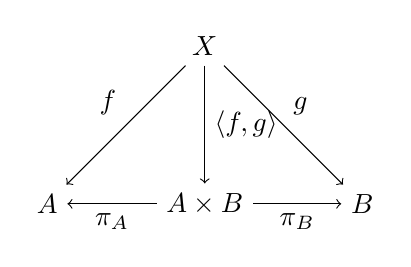
\begin{tikzpicture}[auto]
						\node (a) at (0, 0) {$A$};
						\node (b) at (4, 0) {$B$};
						\node (ab) at (2, 0) {$A\times B$};
						\node (x) at (2, 2) {$X$};
						\draw[->] (ab) to node {$\pi_A$}(a);
						\draw[->] (ab) to node[swap] {$\pi_B$}(b);
						\draw[->] (x) to node[swap] {$f$}(a);
						\draw[->] (x) to node {$g$}(b);
						\draw[->] (x) to node {$\tuple{f,g}$}(ab);
					\end{tikzpicture}
				\end{center}
				\item[積$(P,\rho_A,\rho_B)$の性質]
				積$P$と射影射$\mor{\rho_A}{P}{A}$、$\mor{\rho_B}{P}{B}$において二つの射$\mor{f}{X}{A}$、$\mor{g}{X}{B}$に対する射の対を$\mor{[f,g]}{X}{P}$とする。また射$[f,g]$が積$P$における射の対であるとき、
				\begin{align*}
					\rho_A\circ[f,g]&=f\\
					\rho_B\circ[f,g]&=g
				\end{align*}
				が成り立つ。
				またこのような射の対は一意に存在する。
				\begin{center}
					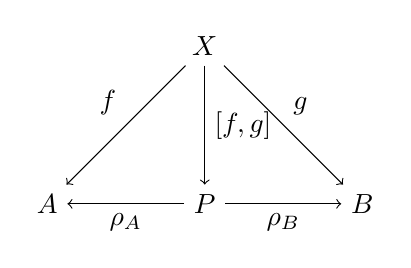
\begin{tikzpicture}[auto]
						\node (a) at (0, 0) {$A$};
						\node (b) at (4, 0) {$B$};
						\node (ab) at (2, 0) {$P$};
						\node (x) at (2, 2) {$X$};
						\draw[->] (ab) to node {$\rho_A$}(a);
						\draw[->] (ab) to node[swap] {$\rho_B$}(b);
						\draw[->] (x) to node[swap] {$f$}(a);
						\draw[->] (x) to node {$g$}(b);
						\draw[->] (x) to node {$[f,g]$}(ab);
					\end{tikzpicture}
				\end{center}
			\end{description}

			積$A\times B$における射の対$\mor{\tuple{f,g}}{X}{A\times B}$に対し、積$P$における射の対$\mor{[f,g]}{X}{P}$は全く別の射である。そのため対の表記で区別することにする。

			また$\pi_A\circ[f,g]=f$は成り立たないどころか、ドメイン、コドメインは$\mor{\pi_A}{A\times B}{A}$と$\mor{[f,g]}{X}{P}$となり合成すらできないということに注意してほしい。
		\end{quote}
		証明に戻ると、\[[\pi_A,\pi_B]\circ\tuple{\rho_A,\rho_B}=id_P\]と
		\[\tuple{\rho_A,\rho_B}\circ[\pi_A,\pi_B]=id_{A\times B}\]が成り立つことを二つの積の普遍性による射の一意性から示せばよい。具体的にはこれらの射がある積の図式における射の対になることを示し、射の対の一意性から等式を導く。

		積$(A\times B,\pi_A,\pi_B)$において、二射$\rho_A,\rho_B$に対する射の対を\[\mor{\tuple{\rho_A,\rho_B}}{P}{A\times B}\]とする。

		逆に積$(P,\rho_A,\rho_B)$において二射$\pi_A,\pi_B$に対する射の対を\[\mor{[\pi_A,\pi_B]}{A\times B}{P}\]とする。
		\begin{center}
			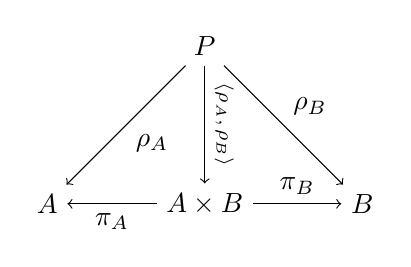
\begin{tikzpicture}[auto]
				\node (a) at (0, 0) {$A$};
				\node (ab) at (2, 0) {$A\times B$};
				\node (b) at (4, 0) {$B$};
				\node (p) at (2, 2) {$P$};
				\draw[->] (p) to node{$\rho_A$}(a);
				\draw[->] (p) to node{$\rho_B$}(b);
				\draw[->] (p) to node[sloped]{\scriptsize{$\tuple{\rho_A,\rho_B}$}}(ab);
				\draw[->] (ab) to node{$\pi_A$}(a);
				\draw[->] (ab) to node{$\pi_B$}(b);
			\end{tikzpicture}
			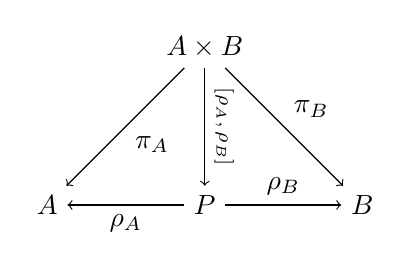
\begin{tikzpicture}[auto]
				\node (a) at (0, 0) {$A$};
				\node (ab) at (2, 2) {$A\times B$};
				\node (b) at (4, 0) {$B$};
				\node (p) at (2, 0) {$P$};
				\draw[->] (p) to node{$\rho_A$}(a);
				\draw[->] (p) to node{$\rho_B$}(b);
				\draw[->] (ab) to node[sloped]{\scriptsize{$[\rho_A,\rho_B]$}}(p);
				\draw[->] (ab) to node{$\pi_A$}(a);
				\draw[->] (ab) to node{$\pi_B$}(b);
			\end{tikzpicture}
		\end{center}
		次に$\mor{\tuple{\rho_A,\rho_B}\circ[\pi_A,\pi_B]}{A\times B}{A\times B}$が$\pi_A$と$\pi_B$の射の対であることを示す。
		\begin{align*}
			\pi_A\circ\tuple{\rho_A,\rho_B}\circ[\pi_A,\pi_B]&=\rho_A\circ[\pi_A,\pi_B]&\text{(積$A\times B$の射の対の可換性)}\\
			&=\pi_A&\text{(積$P$の射の対の可換性)}\\
			\pi_B\circ\tuple{\rho_A,\rho_B}\circ[\pi_A,\pi_B]&=\rho_B\circ[\pi_A,\pi_B]&\text{(積$A\times B$の射の対の可換性)}\\
			&=\pi_B&\text{(積$P$の射の対の可換性)}\\
		\end{align*}
		よって\[\pi_A\circ(\tuple{\rho_A,\rho_B}\circ[\pi_A,\pi_B])=\pi_A,\ \pi_B\circ(\tuple{\rho_A,\rho_B}\circ[\pi_A,\pi_B])=\pi_B\]が成り立つから、$\tuple{\rho_A,\rho_B}\circ[\pi_A,\pi_B]$は射$\pi_A$と$\pi_B$の射の対となる。すると射の対の一意性より、\[\tuple{\rho_A,\rho_B}\circ[\pi_A,\pi_B]=\tuple{\pi_A,\pi_B}=id_{A\times B}\]が成り立つ。
		\begin{center}
			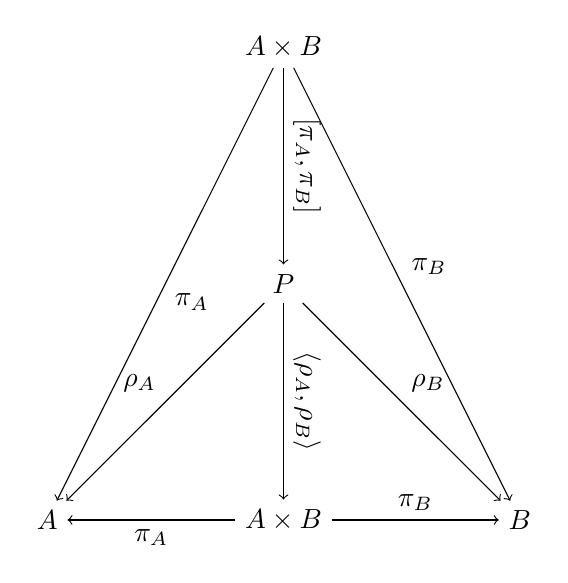
\begin{tikzpicture}[auto]
				\node (a) at (0, 0) {$A$};
				\node (ab) at (3, 0) {$A\times B$};
				\node (ab2) at (3, 6) {$A\times B$};
				\node (b) at (6, 0) {$B$};
				\node (p) at (3, 3) {$P$};
				\draw[->] (p) to node[swap]{$\rho_A$}(a);
				\draw[->] (p) to node{$\rho_B$}(b);
				\draw[->] (p) to node[sloped]{$\tuple{\rho_A,\rho_B}$}(ab);
				\draw[->] (ab2) to node[sloped]{$[\pi_A,\pi_B]$}(p);
				\draw[->] (ab) to node{$\pi_A$}(a);
				\draw[->] (ab) to node{$\pi_B$}(b);
				\draw[->] (ab2) to node{$\pi_A$}(a);
				\draw[->] (ab2) to node{$\pi_B$}(b);
			\end{tikzpicture}
			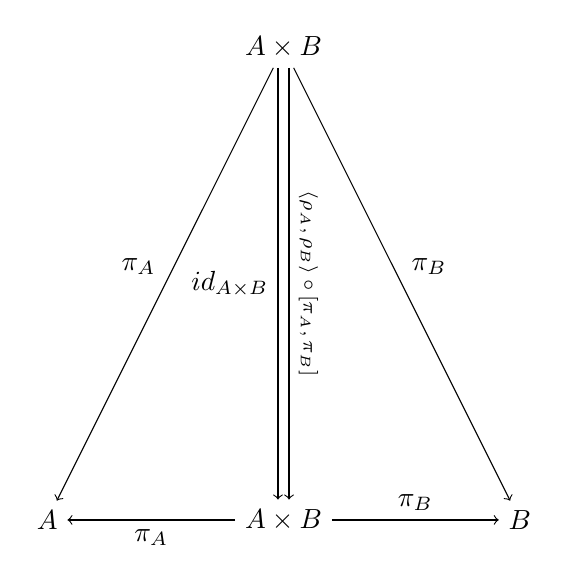
\begin{tikzpicture}[auto]
				\node (a) at (0, 0) {$A$};
				\node (ab) at (3, 0) {$A\times B$};
				\node (b) at (6, 0) {$B$};
				\node (ab2) at (3, 6) {$A\times B$};
				\draw[->] (ab2) to node[swap]{$\pi_A$}(a);
				\draw[->] (ab2) to node{$\pi_B$}(b);
				\draw[->,transform canvas={xshift=2pt}] (ab2) to node[sloped]{\scriptsize{$\tuple{\rho_A,\rho_B}\circ[\pi_A,\pi_B]$}}(ab);
				\draw[->,transform canvas={xshift=-2pt}] (ab2) to node[swap]{$id_{A\times B}$}(ab);
				\draw[->] (ab) to node{$\pi_A$}(a);
				\draw[->] (ab) to node{$\pi_B$}(b);
			\end{tikzpicture}
		\end{center}
		同様に$[\pi_A,\pi_B]\circ\tuple{\rho_A,\rho_B}=id_P$が成り立つから、$[\pi_A,\pi_B]$と$\tuple{\rho_A,\rho_B}$は同型射となり、$A\times B\cong P$が成り立つ。
	\end{proof}

	\subsection{終対象}
	\begin{define}[終対象]
		ある圏$\cat{C}$に終対象が存在するとは、ある対象$1$が存在して圏$\cat{C}$の任意の対象$X$に対し射$\mor{!_X}{X}{1}$が一意に存在するときである。

		元を取る操作とは射の向きが逆であることに注意してほしい。
	\end{define}
	射の対$\mor{\tuple{f,g}}{X}{A\times B}$は対象$X$と射$f,g$に対して一意に存在するのであったが、終対象への射$\mor{!_X}{X}{1}$は対応する射が存在しない。そのため、終対象への射は対象$X$に対して無条件で一意に存在することになる。
	\begin{prop}[終対象から終対象への射]
		終対象から終対象への射は恒等射ただ一つである。
	\end{prop}
	\begin{proof}
		終対象$1$に対して、終対象から終対象への射$\mor{!_1}{1}{1}$は無条件で一意に定まる。
		すべての対象に恒等射は存在するから$id_1=!_1$となる。
		\begin{center}
			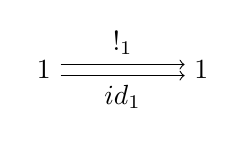
\begin{tikzpicture}[auto]
				\node (1) at (0, 0) {$1$};
				\node (1') at (2, 0) {$1$};
				\draw[->,transform canvas={yshift=2pt}] (1) to node{$!_{1}$}(1');
				\draw[->,transform canvas={yshift=-2pt}] (1) to node[swap]{$id_1$}(1');
			\end{tikzpicture}
		\end{center}
	\end{proof}

	\begin{prop}[終対象の一意性]
		終対象$1$に対して別の終対象$I$が存在するとき、$1\cong I$が成り立つ。
	\end{prop}
	\begin{proof}
		終対象$1$における$I$からの一意に定まる射$\mor{!_I}{I}{1}$と終対象$I$における$1$からの一意に定まる射$\mor{i_1}{1}{I}$の合成$\mor{!_I\circ i_1}{1}{1}$と$\mor{i_1\circ!_I}{I}{I}$はそれぞれ終対象から終対象への射である。

		よって$!_I\circ i_1=id_1$と$i_1\circ!_I=id_I$が成り立ち、$!_I$、$i_1$が同型射になるから$1\cong I$が成り立つ。
		\begin{center}
			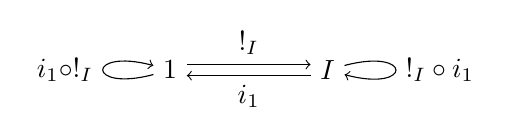
\begin{tikzpicture}[auto]
				\node (1) at (0, 0) {$1$};
				\node (1') at (2, 0) {$I$};
				\draw[->,transform canvas={yshift=2pt}] (1) to node{$!_I$}(1');
				\draw[->,transform canvas={yshift=-2pt}] (1') to node{$i_1$}(1);
				\draw[->,loop left ,looseness=20] (1) to node{$i_1\circ !_I$}(1);
				\draw[->,loop right ,looseness=20] (1') to node{$!_I\circ i_1$}(1');
			\end{tikzpicture}
		\end{center}
	\end{proof}

  最後に終対象と積の二つの普遍性を使った証明を考える。もし余力があれば自力で証明を書いてみてほしい。
  \begin{prop}[終対象との積]
    終対象$1$と任意の対象$A$において、$A\times 1\cong A$が成り立つ。
  \end{prop}
  \begin{proof}
    対象$A$が$1$と$A$に対する積対象であることを示せば良い。より正確には積$(A,id_A,!_A)$が$1,A$に対する積であることを示す。
    また、積$(A,id_A,!_A)$の任意の対象$X$からの二射$\mor{f}{X}{A}$、$\mor{!_X}{X}{1}$に対する射の対を$\mor{f}{X}{A}$とする。
    
    \begin{center}
			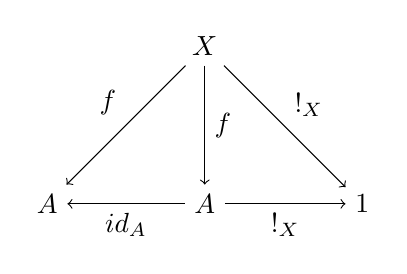
\begin{tikzpicture}[auto]
				\node (a) at (0, 0) {$A$};
				\node (ab) at (2, 0) {$A$};
				\node (b) at (4, 0) {$1$};
				\node (p) at (2, 2) {$X$};
				\draw[->] (p) to node[swap]{$f$}(a);
				\draw[->] (p) to node{$!_X$}(b);
				\draw[->] (p) to node{$f$}(ab);
				\draw[->] (ab) to node{$id_A$}(a);
				\draw[->] (ab) to node[swap]{$!_X$}(b);
			\end{tikzpicture}
    \end{center}

    まずは$f$が射の対であることを確認する。
    \begin{align*}
      id_A\circ f &= f&\text{(恒等射の定義)}\\
      !_A\circ f &= !_X&\text{(終対象の普遍性)}
    \end{align*}
    後者の式は$\mor{!_A\circ f}{X}{1}$と$\mor{!_X}{X}{1}$のどちらも対象$X$からの射であるため、終対象の定義より一意に定まる。よって$f$は確かに$f$と$!_X$の射の対である。

    次に射の対の一意性を示す。
    まずは$f$が射の対であることを確認する。
    同様に$f$と$!_X$の射の対となるような任意の射$f'$は以下の等式を満たす。
    \begin{align*}
      id_A\circ f' &= f\\
      !_A\circ f' &= !_X
    \end{align*}
    前者の等式より、$id_A\circ f'=f'=f$となり、射の対は一意に定まる。

    よって積$(A,id_A,!_A)$は$1$と$A$に対する積であり、積の一意性より$A\times 1\cong A$が成り立つ。

    また証明は省略するが、同型射はそれぞれ$\mor{\tuple{id_A,!_X}}{A}{A\times 1}$、$\mor{\pi_A}{A\times 1}{A}$となる。
  \end{proof}
  \section{集合の圏}

  圏の一例としてこれまで集合の圏を扱ってきたが、一般的な圏の射集合の定義に集合が使われていることからわかるように、集合の圏は圏論の中でも重要な役割を果たす。集合というと、集合論的な操作を想定するかもしれないが、純粋な圏論で使用するいくつかの集合の性質はたいてい圏の言葉で置き換えることができる。そのためこれから扱ういくつかの集合、とりわけ射集合を異質な存在として捉えないようにしていただきたい。

  \subsection{集合の圏と積}
	まずは集合の圏$\cat{Set}$と積の関係性を示す。元を指定して直接直積集合を定義する方法と、普遍性を用いて直積集合の周りの写像の性質を述べて定義する方法の二つが同値であることを確認してほしい。
	\begin{define}[直積集合]
		集合$A$と$B$の直積集合$A\times B$を\[A\times B =\{\tuple{a,b}\ |\ a\in A,\ b\in B\}\]と定義する。
	\end{define}
	\begin{prop}
		集合の圏$\cat{Set}$の対象$A$と$B$の積$A\times B$は集合$A$と$B$の直積集合である。
	\end{prop}
	\begin{proof}
		任意の元$\mor{a}{1}{A}$、$\mor{b}{1}{B}$に対して射の対の存在性により元の対$\mor{\tuple{a,b}}{1}{A\times B}$が存在する。
		また、$A\times B$の任意の元$\mor{f}{1}{A\times B}$は射影射との合成\[\pi_A\circ f=a',\ \pi_B\circ f=b'\]により、何かしらの元$a',b'$に分解できる。この時、射の対の一意性から$f=\tuple{a',b'}$が成り立つから、$f$は元の対であり順序対になる。そのため順序対とならないような元は含まれないことがわかる。

		よって実際に積$A\times B$は集合$A$と$B$の直積集合であることが示せた。
		\begin{center}
			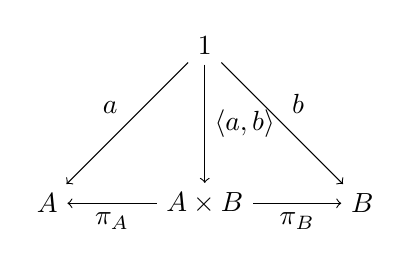
\begin{tikzpicture}[auto]
				\node (a) at (0, 0) {$A$};
				\node (b) at (4, 0) {$B$};
				\node (ab) at (2, 0) {$A\times B$};
				\node (x) at (2, 2) {$1$};
				\draw[->] (ab) to node {$\pi_A$}(a);
				\draw[->] (ab) to node[swap] {$\pi_B$}(b);
				\draw[->] (x) to node[swap] {$a$}(a);
				\draw[->] (x) to node {$b$}(b);
				\draw[->] (x) to node {$\tuple{a,b}$}(ab);
			\end{tikzpicture}
		\end{center}
	\end{proof}

	\begin{prop}
	集合$A$と$B$の直積集合$A\times B$は集合の圏$\cat{Set}$における積である。
	\end{prop}
	\begin{proof}
		限定的ではあるが、まずは任意の対象$X$に終対象$1$を当てはめた場合を見ていき、その後任意の対象$X$に拡張する。
		射影射となる射影写像$\pi_A,\pi_B$を任意の順序対$\tuple{a,b}$において\[\pi_A(\tuple{a,b})=a,\ \pi_B(\tuple{a,b})=b\]と定義する。

		直積集合の定義より、任意の元$a$、$b$に対して順序対$\tuple{a,b}$が存在し、順序対ではない元や重複する元を含まないことから、積の普遍性を部分的に満たすことがわかる。
		\begin{center}
			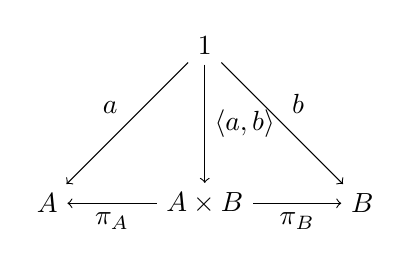
\begin{tikzpicture}[auto]
				\node (a) at (0, 0) {$A$};
				\node (b) at (4, 0) {$B$};
				\node (ab) at (2, 0) {$A\times B$};
				\node (x) at (2, 2) {$1$};
				\draw[->] (ab) to node {$\pi_A$}(a);
				\draw[->] (ab) to node[swap] {$\pi_B$}(b);
				\draw[->] (x) to node[swap] {$a$}(a);
				\draw[->] (x) to node {$b$}(b);
				\draw[->] (x) to node {$\tuple{a,b}$}(ab);
			\end{tikzpicture}
		\end{center}
		次に元の対から写像の対に拡張して考える。写像の対が一意に存在することを元の対が一意に存在することから示せばよい。

		写像$\mor{f}{X}{A}$と写像$\mor{g}{X}{B}$の写像の対$\tuple{f,g}$を$X$の任意の元$x$に対して\[\tuple{f,g}(x)=\tuple{f(x),g(x)}\]と定義する。

		また、
		\begin{align*}
			(\pi_A\circ\tuple{f,g})(x)&=\pi_A(\tuple{f,g}(x))&\text{(写像の合成の定義)}\\
			&=\pi_A(\tuple{f(x),g(x)})&\text{(写像の対の定義)}\\
			&=f(x)&\text{(元の対の可換性)}\\
			(\pi_B\circ\tuple{f,g})(x)&=\pi_B(\tuple{f,g}(x))&\text{(写像の合成の定義)}\\
			&=\pi_B(\tuple{f(x),g(x)})&\text{(写像の対の定義)}\\
			&=g(x)&\text{(元の対の可換性)}
		\end{align*}
		よって\[\pi_A\circ\tuple{f,g}=f,\ \pi_B\circ\tuple{f,g}=g\]が成り立つから写像の対は射の対としての可換性を満たすことがわかる。
		またこのような射の対は$\mor{f}{X}{A}$、$\mor{g}{X}{B}$なる任意の二射$f,g$に対し存在する。

		仮に$\pi_A\circ h=f,\ \pi_B\circ h=g$となる射$\mor{h}{X}{A\times B}$が存在しても、
		$\pi_A(h(x))=f(x),\ \pi_B(h(x))=g(x)$と元の対の一意性より$h(x)=\tuple{f(x),g(x)}$が成り立ち$h=\tuple{f,g}$となる。よって写像$f,g$の写像の対$\tuple{f,g}$は一意に存在する。
		\begin{center}
			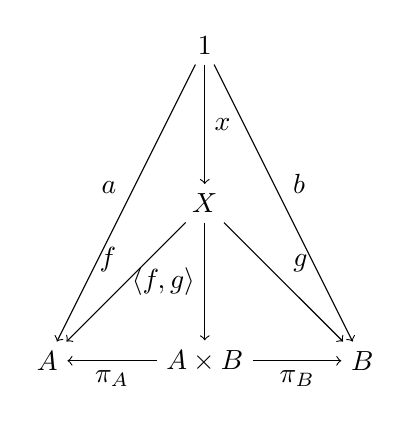
\begin{tikzpicture}[auto]
				\node (a) at (0, 0) {$A$};
				\node (b) at (4, 0) {$B$};
				\node (ab) at (2, 0) {$A\times B$};
				\node (i) at (2, 4) {$1$};
				\node (x) at (2, 2) {$X$};
				\draw[->] (ab) to node {$\pi_A$}(a);
				\draw[->] (ab) to node[swap] {$\pi_B$}(b);
				\draw[->] (x) to node[swap] {$f$}(a);
				\draw[->] (x) to node {$g$}(b);
				\draw[->] (x) to node[swap] {$\tuple{f,g}$}(ab);
				\draw[->] (i) to node[swap] {$a$}(a);
				\draw[->] (i) to node {$b$}(b);
				\draw[->] (i) to node {$x$}(x);
			\end{tikzpicture}
		\end{center}
	\end{proof}
	
  \subsection{集合の圏と終対象}
	\begin{define}[一点集合]
		何かしらの要素をただ一つ持つような集合$\{*\}$を一点集合とする。
	\end{define}
	\begin{prop}
		集合の圏$\cat{Set}$の終対象は一点集合である。
	\end{prop}
	\begin{proof}
		終対象$1$の元、すなわち射$\mor{*}{1}{1}$は終対象から終対象への射であり、恒等射ただ一つであるから終対象の元はただ一つである。
	\end{proof}
	\begin{prop}
		一点集合は集合の圏$\cat{Set}$における終対象である。
	\end{prop}
	\begin{proof}
		任意の集合$A$と一点集合$1$においてある写像$\mor{!_A}{A}{1}$が一意に存在することを示せばよい。
		任意の元$\mor{a}{1}{A}$において$!_A(a)=*$と定義すると、このような写像は任意の集合で定義できることがわかる。
		また一点集合の元がただ一つしかないので、どのような写像であっても任意の元$a$は必ず$*$に対応することになる。つまり$!_A(a)=*$以外の対応付けが行えないので写像$!_A$は一意に存在することがわかる。

		よって$A$から$1$への写像は一意に存在し、一点集合$1$は終対象となる。
	\end{proof}
	次に集合の圏に限定するが、終対象からの射を元とみなせることを証明する。

  \begin{define}[定写像]
    集合の圏$\cat{Set}$において、任意の対象$A,B$と$B$の任意の元$b$に対する定写像を$\mor{\varDelta b}{A}{B}$とし、$A$の任意の元$a$に対して$\varDelta b(a)=b$となる写像とする。
  \end{define}
  定写像は常に一定の値を返す定数関数のような写像である。次に元をその元を返す定写像に写す写像である、対角写像を定義する。
  \begin{define}[対角写像]
    集合の圏$\cat{Set}$において任意の対象$A,B$に対し、対角写像$\mor{\varDelta}{A}{\arset{Set}{B}{A}}$を$\varDelta(a)=\varDelta a$と定義する。すなわち、任意の元$a,b$に対して$\varDelta(a)(b)=a$である。
  \end{define}
	\begin{prop}[集合の元と終対象]
		任意の集合$A$とある一点集合$1$に対し$A\cong\arset{Set}{1}{A}$が成り立つ。
	\end{prop}
	\begin{proof}
    まず一点集合$1$から任意の集合$A$への射が定写像であることを示そう。\\
    これは簡単で一点集合はただ一つの元しか持たないから、それを写した先の元はただ一つに定まる。よって定写像である。\\
    対角写像$\mor{\varDelta}{A}{\arset{Set}{1}{A}}$に逆射$\mor{\varDelta^{-1}}{\arset{Set}{1}{A}}{A}$が存在することを示す。\\
    任意の射$\mor{f}{1}{A}$に対して$\varDelta^{-1}(f)=f(*)$と定義する。すると任意の射$\mor{f}{1}{A}$と任意の元$a$に対して
    \begin{align*}
      (\varDelta^{-1}\circ\varDelta)a&=\varDelta^{-1}(\varDelta a)&\text{(写像の合成の定義)}\\
      &=\varDelta a(*)&\text{($\varDelta^{-1}$の定義)}\\
      &=a&\text{(対角写像の定義)}\\
      (\varDelta\circ\varDelta^{-1})f&=(\varDelta\circ\varDelta^{-1})(\varDelta a)&\text{(fは定写像)}\\
      &=(\varDelta\circ(\varDelta^{-1}\circ\varDelta))(a)&\text{(写像の合成の定義)}\\
      &=\varDelta((\varDelta^{-1}\circ\varDelta)a)&\text{(写像の合成の定義)}\\
      &=\varDelta a&\text{(前式)}\\
      &=f
    \end{align*}
    よって\[\varDelta^{-1}\circ\varDelta=id_A,\ \varDelta\circ\varDelta^{-1}=id_\arset{Set}{1}{A}\]が成り立つから同型射であり、$A\cong\arset{Set}{1}{A}$である。
	\end{proof}

  \subsection{集合の圏と射集合}
	圏を定義する際に使用した射集合だが、射集合も集合であるため集合の圏の対象として捉えることができる。射集合というと、未知の集合論的な操作をいくつも持っているのかと考えてしまうが、これから扱う射集合の性質は圏論的に定義されたものだけで事足りる。そのため少し大げさかもしれないが、これから説明する操作や性質を射集合の定義だと考えても良いかもしれない。
  また、ここから一般の圏$\cat{C}$と集合の圏$\cat{Set}$を同時に扱うことになる。そのため、今扱っている対象や射、議論がどの圏上で行われるのかを意識してほしい。

  \begin{define}[共変射写像]
		圏$\cat{C}$の対象$A,B$と射$\mor{f}{A}{B}$に対して、任意の射$\mor{g}{X}{A}$に射$f$を左から合成する写像を
		\begin{align*}
			&\mor{\arset{C}{X}{f}}{\arset{C}{X}{A}}{\arset{C}{X}{B}}\\
			&\arset{C}{X}{f}(g)=f\circ g
		\end{align*}
		\begin{center}
			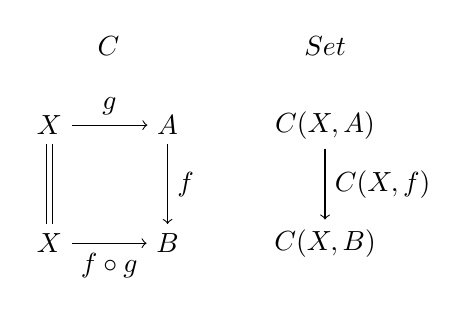
\begin{tikzpicture}[auto]
				\node (x) at (-1.5, 0) {$X$};
				\node (x2) at (-1.5, -1.5) {$X$};
				\node (a) at (0, 0) {$A$};
				\node (b) at (0, -1.5) {$B$};
				\node (ca) at (2, 0) {$\arset{C}{X}{A}$};
				\node (cb) at (2, -1.5) {$\arset{C}{X}{B}$};
				\node (catc) at (-0.75, 1) {$\cat{C}$};
				\node (catc) at (2, 1) {$\cat{Set}$};
				\draw[->] (ca) to node{$\arset{C}{X}{f}$}(cb);
				\draw[->] (a) to node{$f$}(b);
				\draw[double distance=2pt] (x) to (x2);
				\draw[->] (x) to node{$g$}(a);
				\draw[->] (x2) to node[swap]{$f\circ g$}(b);
			\end{tikzpicture}
		\end{center}
		と定義する。
	\end{define}
  
  圏の定義で確認した射の合成を行う写像\[\mor{\circ}{\arset{C}{A}{B}\times\arset{C}{X}{A}}{\arset{C}{X}{B}}\]
  は、任意の射集合の元の対$\tuple{f,g}$を$f\circ g$に写す写像であったが、共変射写像$\arset{C}{X}{f}$は対の左側の射$f$を固定した写像であることがわかる。

  本題から少し外れるが、射集合の元の対$\tuple{f,g}$は積の普遍性で扱った射の対ではないことに注意してほしい。ただし、条件によっては一対一対応をすることがある。これは後で証明を行う。

  共変射写像では射を左から合成する写像を考えたが、次は射を右から合成する写像である反変射写像を考える。

	\begin{define}[反変射写像]
		圏$\cat{C}$の対象$A,B$と射$\mor{f}{A}{B}$に対して、任意の射$\mor{g}{X}{B}$に射$f$を右から合成する写像を
		\begin{align*}
			&\mor{\arset{C}{f}{X}}{\arset{C}{B}{X}}{\arset{C}{A}{X}}\\
			&\arset{C}{f}{X}(g)=g\circ f
		\end{align*}
		\begin{center}
			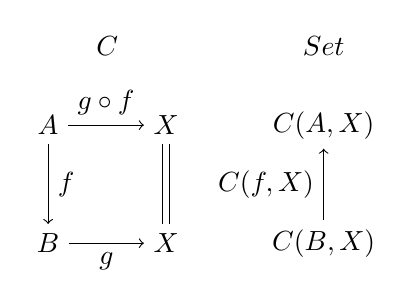
\begin{tikzpicture}[auto]
				\node (x) at (0, 0) {$X$};
				\node (x2) at (0, -1.5) {$X$};
				\node (a) at (-1.5, 0) {$A$};
				\node (b) at (-1.5, -1.5) {$B$};
				\node (ca) at (2, 0) {$\arset{C}{A}{X}$};
				\node (cb) at (2, -1.5) {$\arset{C}{B}{X}$};
				\node (catc) at (-0.75, 1) {$\cat{C}$};
				\node (catc) at (2, 1) {$\cat{Set}$};
				\draw[->] (cb) to node{$\arset{C}{f}{X}$}(ca);
				\draw[->] (a) to node{$f$}(b);
				\draw[double distance=2pt] (x) to (x2);
				\draw[->] (a) to node{$g\circ f$}(x);
				\draw[->] (b) to node[swap]{$g$}(x2);
			\end{tikzpicture}
		\end{center}
		と定義する。共変射写像と違い、射$f$に対して$\arset{C}{f}{X}$の向きが逆になっている。
	\end{define}

  これまでは一般の圏$\cat{C}$の射集合についての議論を行なってきたが、以降は射集合を取る圏を$\cat{Set}$に限定して行うことにする。理由としては$\cat{Set}$上の射集合もまた集合であり、$\cat{Set}$の対象であるためである。そのため、射集合とそのドメイン、コドメインとなる集合の間に射を伸ばすことができ、射集合のさらなる性質を記述することができるようになる。

  次に射写像の応用として、対象の同型との関係性を見る。

  \begin{prop}[同型射となる共変射写像]
    ある圏$\cat{C}$においてある二対象$B\cong B'$が同型であるならば、任意の対象$X$に対し$\arset{C}{X}{B}\cong\arset{C}{X}{B'}$が成り立つ。
  \end{prop}

  \begin{proof}
    同型射を$\mor{i}{B}{B'}$、$\mor{i^{-1}}{B'}{B}$として、共変射写像\[\mor{\arset{C}{X}{i}}{\arset{C}{X}{B}}{\arset{C}{X}{B'}}\]と\[\mor{\arset{C}{X}{i^{-1}}}{\arset{C}{X}{B'}}{\arset{C}{X}{B}}\]もまた同型射になることを示す。すなわち、\[\arset{C}{X}{i}\circ\arset{C}{X}{i^{-1}}=id_{\arset{C}{X}{B'}}\]\[\arset{C}{X}{i^{-1}}\circ\arset{C}{X}{i}=id_{\arset{C}{X}{B}}\]を示せばよい。

    射集合$\arset{C}{X}{B'}$の任意の元$\mor{f}{X}{B'}$に対して、
    \begin{align*}
      \arset{C}{X}{i}\circ\arset{C}{X}{i^{-1}}(f)&=\arset{C}{X}{i}(\arset{C}{X}{i^{-1}}(f))&\text{(写像の合成の定義)}\\
      &=\arset{C}{X}{i}(i^{-1}\circ f)&\text{(共変射写像の定義)}\\
      &=i\circ i^{-1}\circ f&\text{(共変射写像の定義)}\\
      &=id_{B'}\circ f&\text{(同型射の定義)}\\
      &=f&\text{(恒等射の定義)}\\
      &=id_{\arset{C}{X}{B'}}(f)&\text{(恒等射の定義)}
    \end{align*}
    よって$\arset{C}{X}{i}\circ\arset{C}{X}{i^{-1}}=id_{\arset{C}{X}{B'}}$が示せた。同様に$\arset{C}{X}{i^{-1}}\circ\arset{C}{X}{i}=id_{\arset{C}{X}{B}}$も示せる。
    
    よって$\mor{\arset{C}{X}{i}}{\arset{C}{X}{B}}{\arset{C}{X}{B'}}$と$\mor{\arset{C}{X}{i^{-1}}}{\arset{C}{X}{B'}}{\arset{C}{X}{B}}$もまた同型射となるため、$\arset{C}{X}{B}\cong\arset{C}{X}{B'}$が成り立つ。
		\begin{center}
			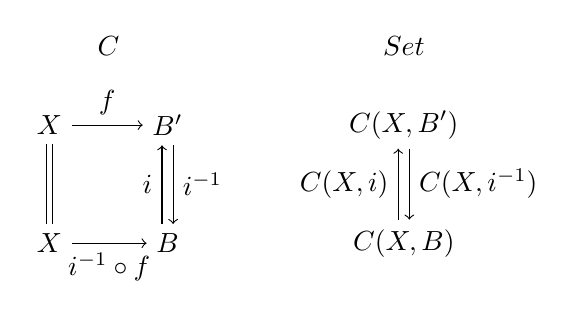
\begin{tikzpicture}[auto]
				\node (x) at (-1.5, 0) {$X$};
				\node (x2) at (-1.5, -1.5) {$X$};
				\node (a) at (0, -1.5) {$B$};
				\node (b) at (0, 0) {$B'$};
				\node (ca) at (3, -1.5) {$\arset{C}{X}{B}$};
				\node (cb) at (3, 0) {$\arset{C}{X}{B'}$};
				\node (catc) at (-0.75, 1) {$\cat{C}$};
				\node (catc) at (3, 1) {$\cat{Set}$};
				\draw[->,transform canvas={xshift=-2pt}] (ca) to node{$\arset{C}{X}{i}$}(cb);
        \draw[->,transform canvas={xshift=2pt}] (cb) to node{$\arset{C}{X}{i^{-1}}$}(ca);
				\draw[->,transform canvas={xshift=-2pt}] (a) to node{$i$}(b);
        \draw[->,transform canvas={xshift=2pt}] (b) to node{$i^{-1}$}(a);

				\draw[double distance=2pt] (x) to (x2);
				\draw[->] (x2) to node[swap]{$i^{-1}\circ f$}(a);
				\draw[->] (x) to node{$f$}(b);
			\end{tikzpicture}
		\end{center}
  \end{proof}
  
  また同様の性質が反変射写像でも成り立つ
  \begin{prop}[同型射となる反変射写像]
    ある圏$\cat{C}$においてある二対象$A\cong A'$が同型であるならば、任意の対象$X$に対し$\arset{C}{A}{X}\cong\arset{C}{A'}{X}$が成り立つ。
  \end{prop}
  
  これはつまり、対象$B$からの射、$B$への射は対象$B'$への射、$B'$からの射と一対一対応をするということである。
  \begin{define}[評価射]
		集合の圏$\cat{Set}$の任意の対象$A,B$と$B$の元$b$、$\cat{Set}$の射$\mor{f}{B}{A}$に対して評価射を
		\begin{align*}
			\mor{&ev_{A,B}}{\arset{Set}{B}{A}\times B}{A}\\
			&ev_{A,B}(\tuple{f,b})=f(b)\\
		\end{align*}
		と定義する。もしくは
    これは元$b$に写像$f$を適用する操作を写像にしたものである。またこのような射は任意の対象$A,B$に対して個別に存在するが、現段階では添え字としての対象を省略し、特に区別はしない。
		厳密な証明は行わないが評価射は実際に写像になる。
	\end{define}

	\begin{define}[余評価射]
		集合の圏$\cat{Set}$の任意の対象$A,B$と$A$の元$a$に対して余評価射を
		\begin{align*}
			\mor{&ce_{A,B}}{A}{\arset{Set}{B}{A\times B}}\\
			&ce_{A,B}(a)=\lambda x.\tuple{a,x}\mor{}{B}{A\times B}\\
			&\lambda x.\tuple{a,x}(b)=\tuple{a,b}
		\end{align*}
		と定義する。また\[ce_{A,B}(a)(b)=\tuple{a,b}\]とも表記できる。
    同様にこのような射は任意の対象$A,B$に対して個別に存在するが区別しない。
	\end{define}

  また、余評価射によって得られる射$\mor{\lambda x.\tuple{a,x}}{B}{A\times B}$と任意の射$\mor{f}{C}{B}$、$\mor{g}{A\times B}{C}$との合成に対して以下の表記を導入する。
  \begin{center}
    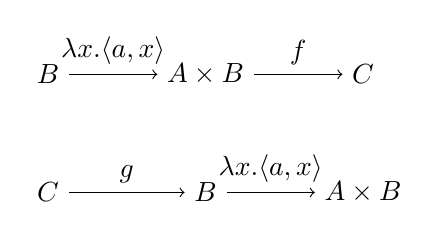
\begin{tikzpicture}[auto]
      \node (c) at (0, 0) {$C$};
      \node (b) at (2, 0) {$B$};
      \node (ab) at (4, 0) {$A\times B$};
      \draw[->] (c) to node{$g$}(b);
      \draw[->] (b) to node{$\lambda x.\tuple{a,x}$}(ab);

      \node (b) at (0, 1.5) {$B$};
      \node (ab) at (2, 1.5) {$A\times B$};
      \node (c) at (4, 1.5) {$C$};
      \draw[->] (b) to node{$\lambda x.\tuple{a,x}$}(ab);
      \draw[->] (ab) to node{$f$}(c);
    \end{tikzpicture}
  \end{center}
  \begin{align*}
    (\lambda x.\tuple{a,x})\circ f &=\lambda x.\tuple{a,f(x)}\\
    g\circ(\lambda x.\tuple{a,x}) &=\lambda x.g(\tuple{a,x})
  \end{align*}

  定義からわかるように、$B$の任意の値$b$を適用すると、
  \begin{align*}
    \lambda x.\tuple{a,f(x)}(b)&=\tuple{a,f(b)}\\
    \lambda x.g(\tuple{a,x})(b)&=g(\tuple{a,b})
  \end{align*}
  となる。
  余評価射の定義に値の適用を用いたが、これは評価射で表すことができる。次はこのような評価射と余評価射の関係性、性質を見ていく。以下証明する二つの命題は当分使用しないため、興味がなければ飛ばしてもらっても構わない。

  \begin{prop}[冪の三角恒等式1]
    任意の対象$A,B$において、\[ce\circ \arset{Set}{B}{ev}=id_{\arset{Set}{B}{A}}\]が成り立つ。
    \begin{center}
			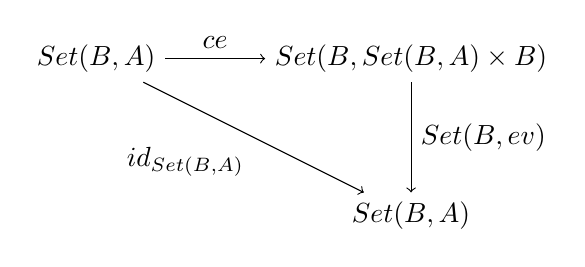
\begin{tikzpicture}[auto]
				\node (setba1) at (0, 0) {$\arset{Set}{B}{A}$};
        \node (setbbab) at (4, 0) {$\arset{Set}{B}{\arset{Set}{B}{A}\times B}$};
				\node (setba2) at (4, -2) {$\arset{Set}{B}{A}$};

				\draw[->] (setba1) to node[swap]{$id_{\arset{Set}{B}{A}}$}
        (setba2);
        \draw[->] (setba1) to node{$ce$}(setbbab);
        \draw[->] (setbbab) to node{$\arset{Set}{B}{ev}$}(setba2);
			\end{tikzpicture}
		\end{center}
  \end{prop}

  \begin{proof}
    任意の射$\mor{f}{B}{A}$に対して、
    \begin{align*}
      \arset{Set}{B}{ev}\circ ce(f)&=\arset{Set}{B}{ev}(\lambda x.\tuple{f,x})&\text{(余評価射の定義)}\\
      &=ev\circ\lambda x.\tuple{f,x}&\text{(共変射写像の定義)}\\
      &=\lambda x.ev(\tuple{f,x})\\
      &=\lambda x.f(x)&\text{(評価射の定義)}
    \end{align*}
    となる。直感的に明らかではあるが、$\lambda x.f(x)=f$を示す。
    対象$B$の任意の元$b$に対して余評価射の定義から\[(\lambda x.f(x))(b)=f(b)\]となる。よって\[\lambda x.f(x)=f\]となり、これが任意の射$f$で成り立つから、
    \[ce\circ \arset{Set}{B}{ev}=id_{\arset{Set}{B}{A}}\]となる。
  \end{proof}

  \begin{prop}[冪の三角恒等式2]
    任意の対象$A,B$において、\[ev\circ(ce\times id_B)=id_{A\times B}\]が成り立つ。
    \begin{center}
			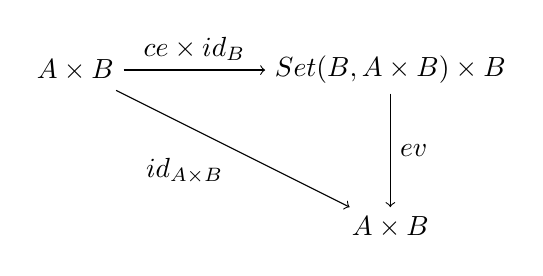
\begin{tikzpicture}[auto]
				\node (setba1) at (0, 0) {$A\times B$};
        \node (setbbab) at (4, 0) {$\arset{Set}{B}{A\times B}\times B$};
				\node (setba2) at (4, -2) {$A\times B$};

				\draw[->] (setba1) to node[swap]{$id_{A\times B}$}
        (setba2);
        \draw[->] (setba1) to node{$ce\times id_B$}(setbbab);
        \draw[->] (setbbab) to node{$ev$}(setba2);
			\end{tikzpicture}
		\end{center}
  \end{prop}

  \begin{proof}
    対象$A\times B$の任意の元$\tuple{a,b}$に対して、
    \begin{align*}
      ev\circ (ce\times id_B)(\tuple{a,b})
      &=ev(\tuple{ce(a),b})&\text{(射の積の定義)}\\
      &=ev(\tuple{\lambda x.\tuple{a,x},b})&\text{(余評価射の定義)}\\
      &=\lambda x.\tuple{a,x}(b)&\text{(評価射の定義)}\\
      &=\tuple{a,b}&\text{(余評価射の定義)}
    \end{align*}
    となる。よって\[ev\circ(ce\times id_B)=id_{A\times B}\]が成り立つ。
  \end{proof}

  \subsection{評価射、余評価射の応用}
  評価射、余評価射を用いれば、集合の圏における圏の定義に現れる操作と等しくなるような写像を構成することができる。ここでは恒等射を得る操作と対角写像の構成を示すが、射の合成を行う操作$\mor{\circ}{\arset{Set}{B}{C}\times \arset{Set}{A}{B}}{\arset{Set}{A}{C}}$を構成することもできる。
  \begin{prop}[余評価射による恒等射の定義]
    $\mor{\arset{Set}{A}{\pi_A}\circ ce}{1}{\arset{Set}{A}{A}}$は射集合$\arset{Set}{A}{A}$における恒等射を表す元である。

    \begin{center}
			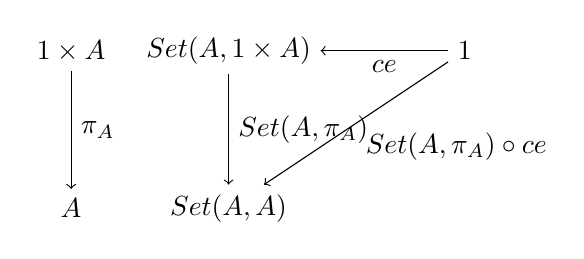
\begin{tikzpicture}[auto]
				\node (1a) at (0, 2) {$1\times A$};
        \node (a) at (0, 0) {$A$};
				\node (s1a) at (2, 2) {$\arset{Set}{A}{1\times A}$};
        \node (sa) at (2, 0) {$\arset{Set}{A}{A}$};
				\node (1) at (5, 2) {$1$};

				\draw[->] (1a) to node{$\pi_A$}(a);
        \draw[->] (s1a) to node{$\arset{Set}{A}{\pi_A}$}(sa);
        \draw[->] (1) to node{$ce$}(s1a);
        \draw[->] (1) to node{$\arset{Set}{A}{\pi_A}\circ ce$}(sa);

			\end{tikzpicture}
		\end{center}

  \end{prop}
  \begin{proof}
    $\arset{Set}{A}{\pi_A}\circ ce(*)$を計算すれば良い。\\
    \begin{align*}
      \arset{Set}{A}{\pi_A}\circ ce(*)&=\arset{Set}{A}{\pi_A}(\lambda x.\tuple{*,x})&\text{(写像の合成の定義)}\\
      &=\pi_A\circ\lambda x.\tuple{*,x}&\text{(射写像の定義)}\\
      &=\lambda x.\pi_A(\tuple{*,x})\\
      &=\lambda x.x\\
    \end{align*}
    余評価射の定義より任意の$A$の元$a$に対して$(\lambda x.x)(a)=a$であるから、$\arset{Set}{A}{\pi_A}\circ ce(*)=id_A$である。
  \end{proof}
  \begin{prop}[余評価射による対角写像の定義]
    対角写像$\mor{\varDelta}{A}{\arset{Set}{B}{A}}$に対して、\[\varDelta=\arset{Set}{B}{\pi_A}\circ ce\]である。
    \begin{center}
			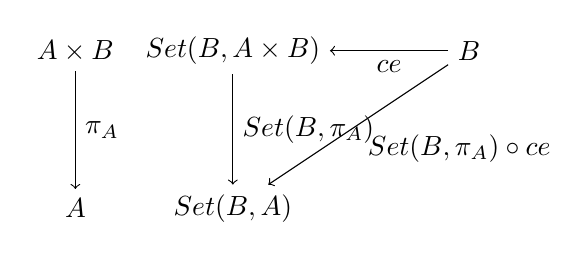
\begin{tikzpicture}[auto]
				\node (1a) at (0, 2) {$A\times B$};
        \node (a) at (0, 0) {$A$};
				\node (s1a) at (2, 2) {$\arset{Set}{B}{A\times B}$};
        \node (sa) at (2, 0) {$\arset{Set}{B}{A}$};
				\node (1) at (5, 2) {$B$};

				\draw[->] (1a) to node{$\pi_A$}(a);
        \draw[->] (s1a) to node{$\arset{Set}{B}{\pi_A}$}(sa);
        \draw[->] (1) to node{$ce$}(s1a);
        \draw[->] (1) to node{$\arset{Set}{B}{\pi_A}\circ ce$}(sa);
			\end{tikzpicture}
		\end{center}
  \end{prop}
  \begin{proof}
    $A$の任意の元$a$に対して、
    \begin{align*}
      \arset{Set}{B}{\pi_A}\circ ce(a)&=\arset{Set}{B}{\pi_A}(\lambda x.\tuple{a,x})&\text{(写像の合成の定義)}\\
      &=\pi_A\circ\lambda x.\tuple{a,x}&\text{(射写像の定義)}\\
      &=\lambda x.\pi_A(\tuple{a,x})\\
      &=\lambda x.a
    \end{align*}
    恒等射と同様に、$B$の任意の元$b$に対して$\mor{\lambda x.a}{B}{A}$は$(\lambda x.a)b=a$を満たす。よって$\lambda x.a$は定写像であり、$\lambda x.a=\varDelta (a)$である。\\
    $\arset{Set}{B}{\pi_A}\circ ce(a)=\varDelta (a)$が成り立つから、$\varDelta=\arset{Set}{B}{\pi_A}\circ ce$である。
  \end{proof}
  \section{関手}
  これまで、似たような性質を持つ対象や射を同時に扱う時、それらの対象に添字をつけて量化してきた。対象の量化の例として積対象$A\times B$は圏$\cat{C}$の任意の対象$A$と任意の対象$B$によって添字づけられている。また射の量化の例として、射の積$\mor{f\times g}{\tuple{A,B}}{\tuple{A',B'}}$は圏$\cat{C}$の任意の射$\mor{f}{A}{A'}$、$\mor{g}{B}{B'}$によって添字づけられている。

  この章では主に、この添字づけを行うような操作を圏から圏への特殊な写像である関手で一般化する。

	\begin{define}
		ある圏$\cat{C}$からある圏$\cat{D}$への関手$\functor{F}{C}{D}$は以下の関数と公理から構成される。
		\begin{quote}
			\begin{description}
		\item[対象関数]$\cat{C}$の対象$A$に$\cat{D}$の対象$FA$を割り当てる対象関数\[\mor{F}{\obj{C}}{\obj{D}}\]
		\item[射関数]$\cat{C}$の任意の各対象$A,B$において射$\mor{f}{A}{B}$に圏$\cat{D}$の射$\mor{Ff}{FA}{FB}$を割り当てる射関数\[\mor{F_{A,B}}{\arset{C}{A}{B}}{\arset{D}{FA}{FB}}\]対象$A,B$に対してそれぞれ存在する射関数$F_{A,B}$を総称して$F$と呼ぶことにする。

		つまり、圏$\cat{C}$に含まれる任意の射$\mor{f}{A}{B}$、$\mor{k}{X}{Y}$に対して\[F(f)=F_{A,B}(f)\]\[F(k)=F_{X,Y}(k)\]と置き換えてほしい。
		また対象関数と射関数は記法で区別しないことと、$Tf,TA$ののように括弧を省略する場合もある。
		\item[恒等射の保存] 射関数は圏$\cat{C}$の恒等射を$\cat{D}$の恒等射に対応させる。つまり$F(id_A)=id_{FA}$が成り立つ。
		\item[射の合成の保存]$\cod(f)=\dom(g)$であるとき、$F(g\circ f)=Fg\circ Ff$が成り立つ。
		\end{description}
		\end{quote}
	\end{define}

  次に関手の具体例を示す。
  以下の射と対象で構成される圏$\cat{C},\cat{D}$と二つの関手$\functor{T}{C}{D}$、$\functor{S}{C}{D}$を考える。
  \begin{center}
    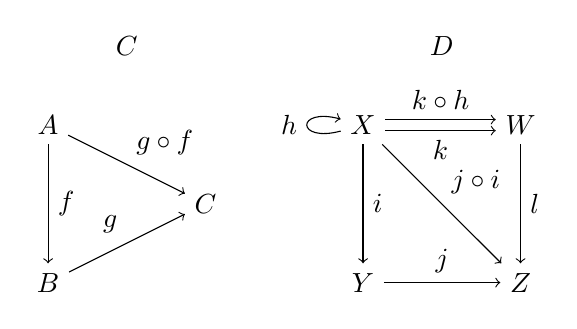
\begin{tikzpicture}[auto]
      \node (a) at (0, 2) {$A$};
      \node (b) at (0, 0) {$B$};
      \node (c) at (2, 1) {$C$};
      \draw[->] (a) to node{$f$}(b);
      \draw[->] (b) to node{$g$}(c);
      \draw[->] (a) to node{$g\circ f$}(c);

      \node (x) at (4, 2) {$X$};
      \node (y) at (4, 0) {$Y$};
      \node (w) at (6, 2) {$W$};
      \node (z) at (6, 0) {$Z$};
      \draw[->] (x) to node{$i$}(y);
      \draw[->] (y) to node{$j$}(z);
      \draw[->] (x) to node{$j\circ i$}(z);
      \draw[->] (w) to node{$l$}(z);
      \draw[->,transform canvas={yshift=-2pt}] (x) to node[swap]{$k$}(w);
      \draw[->,transform canvas={yshift=2pt}] (x) to node{$k\circ h$}(w);
      \draw[->,loop left ,looseness=10] (x) to node{$h$}(x);

      \node (catc) at (1, 3) {$\cat{C}$};
      \node (catd) at (5, 3) {$\cat{D}$};
      %\draw[->,bend right = 15] (catc) to node{$T$}(catd);
      %\draw[->,bend left = 15] (catc) to node{$S$}(catd);
    \end{tikzpicture}
  \end{center}
  そして関手$T$の対象関数$T$を\[T(A)=X,\ T(B)=Y,\ T(C)=Z\]、関手$S$の対象関数$S$を\[S(A)=X,\ S(B)=X,\ S(C)=W\]と定義する。

  次に、関手$T$の射関数$T$を\[T(f)=i,\ T(g)=j,\ T(g\circ f)=j\circ i\]と定義する。また各対象の恒等射の対応は
  \begin{align*}
    T(id_A)&=id_{TA}\\
    &=id_{X}\text{($TA=X$)}\\
    T(id_B)&=id_{TB}\\
    &=id_{Y}\text{($TB=Y$)}\\
    T(id_C)&=id_{TC}\\
    &=id_{Z}\text{($TC=Z$)}
  \end{align*}とする。
  \begin{center}
    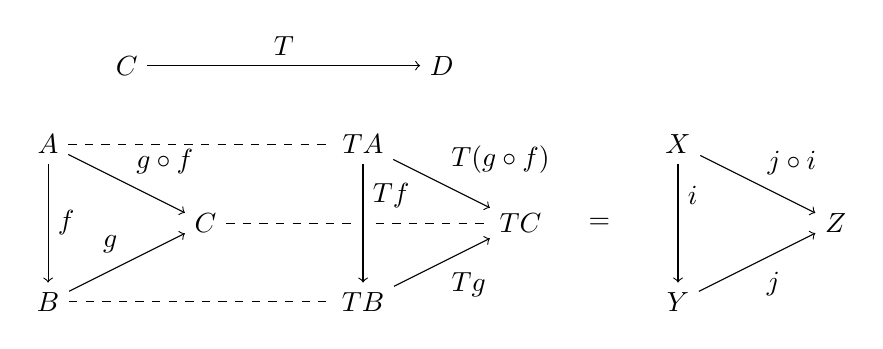
\begin{tikzpicture}[auto]
      \node (a) at (0, 2) {$A$};
      \node (b) at (0, 0) {$B$};
      \node (c) at (2, 1) {$C$};
      \node (ta) at (4, 2) {$TA$};
      \node (tb) at (4, 0) {$TB$};
      \node (tc) at (6, 1) {$TC$};
      \node (x) at (8, 2) {$X$};
      \node (y) at (8, 0) {$Y$};
      \node (z) at (10, 1) {$Z$};

      \node (e) at (7, 1) {$=$};

      \draw[-,dashed] (a) to (ta);
      \draw[-,dashed] (b) to (tb);
      \draw[-,dashed] (c) to (tc);

      \draw[->] (a) to node{$f$}(b);
      \draw[->] (b) to node{$g$}(c);
      \draw[->] (a) to node{$g\circ f$}(c);

      \draw[-, line width=4pt,draw=white] (x) to (y);
      \draw[->] (x) to node[yshift =10]{$i$}(y);
      \draw[->] (y) to node[swap]{$j$}(z);
      \draw[->] (x) to node{$j\circ i$}(z);

      \draw[-, line width=4pt,draw=white] (ta) to (tb);
      \draw[->] (ta) to node[yshift =10]{$Tf$}(tb);
      \draw[->] (tb) to node[swap]{$Tg$}(tc);
      \draw[->] (ta) to node{$T(g\circ f)$}(tc);

      \node (catc) at (1, 3) {$\cat{C}$};
      \node (catd) at (5, 3) {$\cat{D}$};
      \draw[->] (catc) to node{$T$}(catd);

    \end{tikzpicture}
  \end{center}
  この図での点線は対象の写像的な対応を表しているのであって、実際に射が存在するわけではないことに注意してほしい。

  同様に関手$S$の射関数$S$を\[S(f)=h,\ S(g)=k,\ S(g\circ f)=k\circ h\]と定義する。
  恒等射の対応は
  \begin{align*}
    S(id_A)&=id_{SA}\\
    &=id_{X}\text{($SA=X$)}\\
    S(id_B)&=id_{SB}\\
    &=id_{X}\text{($SB=X$)}\\
    S(id_C)&=id_{SC}\\
    &=id_{W}\text{($SC=W$)}
  \end{align*}
  とする。
  \begin{center}
    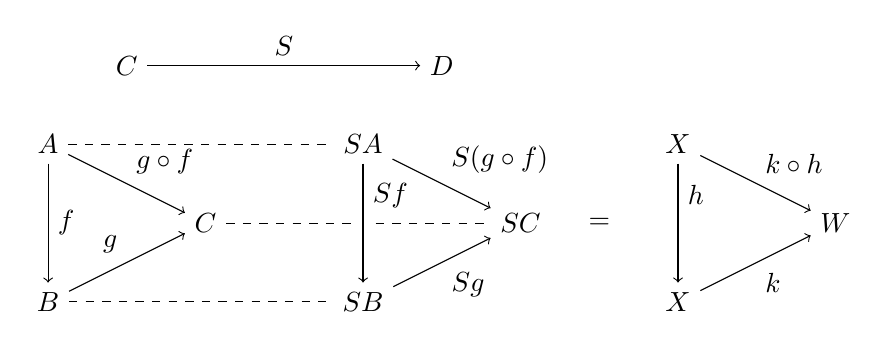
\begin{tikzpicture}[auto]
      \node (a) at (0, 2) {$A$};
      \node (b) at (0, 0) {$B$};
      \node (c) at (2, 1) {$C$};
      \node (ta) at (4, 2) {$SA$};
      \node (tb) at (4, 0) {$SB$};
      \node (tc) at (6, 1) {$SC$};
      \node (x) at (8, 2) {$X$};
      \node (y) at (8, 0) {$X$};
      \node (z) at (10, 1) {$W$};

      \node (e) at (7, 1) {$=$};

      \draw[-,dashed] (a) to (ta);
      \draw[-,dashed] (b) to (tb);
      \draw[-,dashed] (c) to (tc);

      \draw[->] (a) to node{$f$}(b);
      \draw[->] (b) to node{$g$}(c);
      \draw[->] (a) to node{$g\circ f$}(c);

      \draw[-, line width=4pt,draw=white] (x) to (y);
      \draw[->] (x) to node[yshift =10]{$h$}(y);
      \draw[->] (y) to node[swap]{$k$}(z);
      \draw[->] (x) to node{$k\circ h$}(z);

      \draw[-, line width=4pt,draw=white] (ta) to (tb);
      \draw[->] (ta) to node[yshift =10]{$Sf$}(tb);
      \draw[->] (tb) to node[swap]{$Sg$}(tc);
      \draw[->] (ta) to node{$S(g\circ f)$}(tc);

      \node (catc) at (1, 3) {$\cat{C}$};
      \node (catd) at (5, 3) {$\cat{D}$};
      \draw[->] (catc) to node{$S$}(catd);
    \end{tikzpicture}
  \end{center}

  関手$S$、$T$が恒等射を保つことは恒等射の定義から用意に分かる。また、恒等射の合成は省略するが、射の合成の保存は
  \begin{align*}
    T(g\circ f)&=j\circ i&\text{($T(g\circ f)$の定義)}\\
    &=Tg\circ Tf&\text{($Tg,Tf$の定義)}\\
    S(g\circ f)&=k\circ h&\text{($S(g\circ f)$の定義)}\\
    &=Sg\circ Sf&\text{($Sg,Sf$の定義)}
  \end{align*}
  が成り立つことから分かる。

  関手$T$の例で言えば、圏$\cat{D}$の対象$X$は$TA$として圏$\cat{C}$の対象$A$によって添字付けられた対象であると考えられる。また、$X$は別の関手$S$によって$SA,SB$として添字付けられていると考えることもできる。

	\begin{define}[関手の同一性]
		関手$\functor{F,G}{C}{D}$が同一、$F=G$であるとは、それぞれの対象関数、射関数が写像として等しいということである。
	\end{define}


	\begin{prop}[図式の圏論的な定義]
		添字圏と呼ばれる圏$\cat{J}$から図式を取りたい圏$\cat{C}$への関手は図式である。
		例えば以下のように対象$I,J,K$と射$i,j$で構成される添字圏$J$を図式の骨組み、関手$\functor{F}{I}{C}$を図式の骨組みに圏$C$の対象と射を割り当てる操作とする。

		すると関手の合成の保存より、図式中の射$f,g$の合成射$g\circ f$は図式に必ず存在する。
    また恒等射の保存より、図式中の対象に必ず恒等射となる射が存在し、関手の合成の保存により実際に恒等射のように振る舞う。

    このように関手の性質によって、図式はそれ単体で圏のように振る舞う。
		\begin{center}
			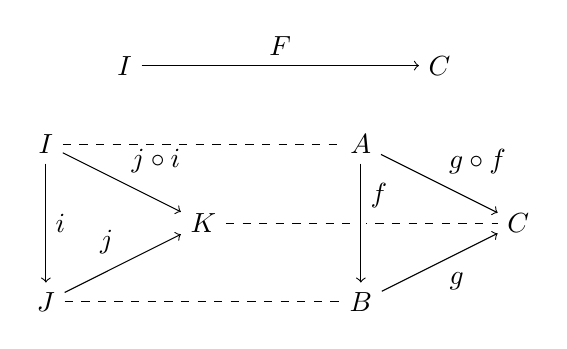
\begin{tikzpicture}[auto]
				\node (a) at (0, 2) {$I$};
				\node (b) at (0, 0) {$J$};
				\node (c) at (2, 1) {$K$};
				\node (x) at (4, 2) {$A$};
				\node (y) at (4, 0) {$B$};
				\node (z) at (6, 1) {$C$};
				\draw[-,dashed] (a) to (x);
				\draw[-,dashed] (b) to (y);
				\draw[-,dashed] (c) to (z);

				\draw[->] (a) to node{$i$}(b);
				\draw[->] (b) to node{$j$}(c);
				\draw[->] (a) to node{$j\circ i$}(c);

				\draw[-, line width=4pt,draw=white] (x) to (y);
				\draw[->] (x) to node[yshift =10]{$f$}(y);
				\draw[->] (y) to node[swap]{$g$}(z);
				\draw[->] (x) to node{$g\circ f$}(z);
				\node (catc) at (1, 3) {$\cat{I}$};
				\node (catd) at (5, 3) {$\cat{C}$};
				\draw[->] (catc) to node{$F$}(catd);

			\end{tikzpicture}
		\end{center}
	\end{prop}
  次に最初に述べた積対象$A\times B$の添字づけについて実際に関手で定式化する。
  ただし、積対象$A\times B$は二つの対象$A,B$によって添字付けられているが、今回は対象$A$にだけを量化し、対象$B$を固定して考える。
	\begin{define}[積関手]
		圏$\cat{C}$が積を持つとき、以下の関数で構成されるある対象$B$に対して圏$C$から圏$C$への関手$\functor{-\times B}{C}{C}$を積関手と呼ぶ。
		\begin{quote}
			\begin{description}
			\item[対象関数] 対象関数を$(-\times B)(A)=A\times B$と定義する。
			\item[射関数] 圏$C$の任意の対象$A,A'$に対する関数$(-\times B)_{A,A'}$を任意の射$\mor{f}{A}{A'}$に対して
			\begin{align*}
				(-\times B)_{A,A'}(f)&=\mor{f\times id_B}{(-\times B)(A)}{(-\times B)(A)}\\
				&=\mor{f\times id_B}{A\times B}{A'\times B}
			\end{align*}
			と定義する。同様に任意の対象$A,A'$に対して存在する射関数$(-\times B)_{A,A'}$を総称して$(-\times B)$と呼ぶ。
			\begin{center}
				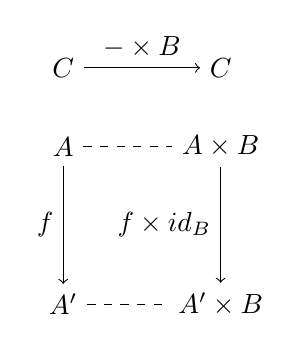
\begin{tikzpicture}[auto]
					\node (a) at (0, 2) {$A$};
					\node (a') at (0, 0) {$A'$};
					\node (ab) at (2, 2) {$A\times B$};
					\node (a'b) at (2, 0) {$A'\times B$};
					\node (catc1) at (0, 3) {$\cat{C}$};
					\node (catc2) at (2, 3) {$\cat{C}$};
					\draw[-,dashed] (a) to (ab);
					\draw[-,dashed] (a') to (a'b);

					\draw[->] (catc1) to node{$-\times B$}(catc2);
					\draw[->] (a) to node[swap]{$f$}(a');
					\draw[->] (ab) to node[swap]{$f\times id_B$}(a'b);
				\end{tikzpicture}
			\end{center}
			\item[恒等射の保存] 射影射の対が恒等射になることを用いて$(-\times B)(id_A)=id_{(-\times B)(A)}$を示せばよい。
			\begin{align*}
				(-\times B)(id_A)&=id_A\times id_B&\text{(射関数の定義)}\\
				&=\tuple{id_A\circ\pi_A,id_B\circ\pi_B}&\text{(射の積の定義)}\\
				&=\tuple{\pi_A,\pi_B}&\text{(恒等射の性質)}\\
				&=id_{A\times B}&\text{(射影射の対)}\\
				&=id_{(-\times B)(A)}&\text{(対象関数の定義)}
			\end{align*}
			よって積関手は恒等射を保つことが示せた。
			\item[射の合成の保存]任意の対象$A,A',A''$と任意の射$\mor{f}{A}{A'},\mor{f'}{A'}{A''}$に対して\[(-\times B)(f'\circ f)=(-\times B)(f')\circ(-\times B)(f)\]が成り立つことを、積と合成の交換から示す。
			\begin{align*}
				(-\times B)(f'\circ f)&=(f'\circ f)\times id_B&\text{(射関数の定義)}\\
				&=(f'\circ f)\times (id_B\circ id_B)&\text{(恒等射の性質)}\\
				&=(f'\times id_B)\circ(f\times id_B)&\text{(積と合成の交換)}\\
				&=(-\times B)(f')\circ(-\times B)(f)&\text{(射関数の定義)}
			\end{align*}
			\begin{center}
				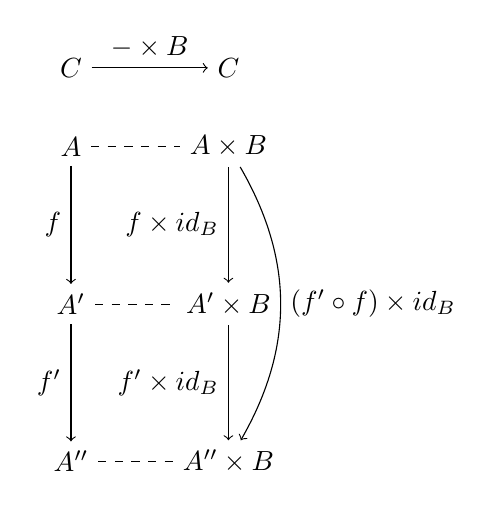
\begin{tikzpicture}[auto]
					\node (a) at (0, 2) {$A$};
					\node (a') at (0, 0) {$A'$};
					\node (a'') at (0, -2) {$A''$};
					\node (ab) at (2, 2) {$A\times B$};
					\node (a'b) at (2, 0) {$A'\times B$};
					\node (a''b) at (2, -2) {$A''\times B$};
					\node (catc1) at (0, 3) {$\cat{C}$};
					\node (catc2) at (2, 3) {$\cat{C}$};
					\draw[-,dashed] (a) to (ab);
					\draw[-,dashed] (a') to (a'b);
					\draw[-,dashed] (a'') to (a''b);
					\draw[->] (catc1) to node{$-\times B$}(catc2);
					\draw[->] (a) to node[swap]{$f$}(a');
					\draw[->] (a') to node[swap]{$f'$}(a'');
					\draw[->] (ab) to node[swap]{$f\times id_B$}(a'b);
					\draw[->] (a'b) to node[swap]{$f'\times id_B$}(a''b);
					\draw[->,bend left =30] (ab) to node{$(f'\circ f)\times id_B$}(a''b);
				\end{tikzpicture}
			\end{center}
			よって積関手は射の合成を保つことが示せた。
		\end{description}
		\end{quote}
	\end{define}
	\begin{prop}[関手の同型の保存]
		任意の圏$\cat{C,D}$と任意の関手$\functor{F}{C}{D}$、圏$\cat{C}$の対象$A,B$において、
		\[A\cong B \Longrightarrow FA\cong FB\]が成り立つ。
	\end{prop}
	\begin{proof}
		同型$A\cong B$のある同型射$\mor{i}{A}{B},\mor{i^{-1}}{B}{A}$に対して$\mor{Fi}{FA}{FB},\mor{Fi^{-1}}{FB}{FA}$も同様に同型射であることを示せばよい。

		\begin{align*}
			Fi^{-1}\circ Fi&=F(i^{-1}\circ i)&\text{($F$の射の合成の保存)}\\
			&=F(id_A)&\text{(恒等射の定義)}\\
			&=id_{FA}&\text{($F$の恒等射の保存)}\\
			Fi\circ Fi^{-1}&=F(i\circ i^{-1})&\text{($F$の射の合成の保存)}\\
			&=F(id_B)&\text{(恒等射の定義)}\\
			&=id_{FB}&\text{($F$の恒等射の保存)}\\
		\end{align*}
		$Fi^{-1}\circ Fi=id_{FA}$、$Fi\circ Fi^{-1}=id_{FB}$より、$Fi,Fi^{-1}$が同型射なる。
		よって$FA\cong FB$が成り立つ。
	\end{proof}

	\subsection{小さい圏の圏}
	関手は圏から圏への一種の写像であるため、集合の圏のように、圏を対象とし関手を射とするような圏である圏の圏を考えることができそうである。
	そのためにもまずは合成射、恒等射にあたる関手を定義していく。
	\begin{define}[合成関手]
		関手$\functor{F}{C}{C'}$、$\functor{G}{C'}{C''}$を合成した関手$\functor{G\circ F}{C}{C'}$を以下の要素によって定義する。
		\begin{quote}
			\begin{description}
			\item[対象関数]関手$F,G$のそれぞれの対象関数$F,G$に対して$G\circ F$の対象関数を$G\circ F$と定義する。つまり圏$\cat{C}$の任意の対象$A$に対して\[(G\circ F)(A)=G(FA)\]となるような写像である。
			\item[射関数]関手$F,G$のそれぞれの射関数$F,G$に対して$G\circ F$の射関数を$G\circ F$と定義する。
			つまり圏$\cat{C}$の任意の対象$A,A'$と任意の射$\mor{f}{A}{A'}$に対して\[\mor{(G\circ F)_{}(f)=G(Ff)}{GFA}{GF{A'}}\]となるような写像である。

			各二対象ごとの射関数も見ていくと、関手$F,G$のそれぞれの関数\[\mor{F_{A,A'}}{\arset{C}{A}{A'}}{\arset{C'}{FA}{FA'}}\]\[\mor{G_{FA,FA'}}{\arset{C'}{FA}{FA'}}{\arset{C''}{GFA}{GFA'}}\]に対して$G\circ F$の関数を\[(G\circ F)_{A,A'}=\mor{G_{FA,FA'}\circ F_{A,A'}}{\arset{C}{A}{A'}}{\arset{C''}{GFA}{GFA'}}\]となる。このように関手の合成はそれぞれの関手の対象関数、射関数の合成に還元して考える。

			\begin{center}
				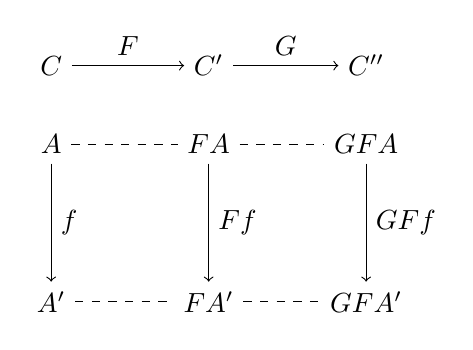
\begin{tikzpicture}[auto]
					\node (a) at (0, 2) {$A$};
					\node (a') at (0, 0) {$A'$};
					\node (fa) at (2, 2) {$FA$};
					\node (fa') at (2, 0) {$FA'$};
					\node (gfa) at (4, 2) {$GFA$};
					\node (gfa') at (4, 0) {$GFA'$};
					\node (catc) at (0, 3) {$\cat{C}$};
					\node (catc') at (2, 3) {$\cat{C'}$};
					\node (catc'') at (4, 3) {$\cat{C''}$};
					\draw[-,dashed] (a) to (fa);
					\draw[-,dashed] (a') to (fa');
					\draw[-,dashed] (fa) to (gfa);
					\draw[-,dashed] (fa') to (gfa');
					\draw[->] (catc) to node{$F$}(catc');
					\draw[->] (catc') to node{$G$}(catc'');

					\draw[->] (a) to node{$f$}(a');
					\draw[->] (fa) to node{$Ff$}(fa');
					\draw[->] (gfa) to node{$GFf$}(gfa');

				\end{tikzpicture}
			\end{center}
			また紛らわしくない場合は合成関手$G\circ F$を$GF$と略すことにする。
			\item[恒等射の保存] $GF(id_A)=id_{GFA}$を示せばよい。
				\begin{align*}
					GF(id_A)&=G(F(id_A))&\text{(射関数の定義)}\\
					&=G(id_{FA})&\text{(関手$F$の恒等射の保存)}\\
					&=id_{GFA}&\text{(関手$G$の恒等射の保存)}
				\end{align*}
			よって合成関手は恒等射を保つ。
			\item[射の合成の保存] $GF(g\circ f)=GFg\circ GFf$を示せばよい。
				\begin{align*}
					GF(g\circ f)&=G(F(g\circ f))&\text{(射関数の定義)}\\
					&=G(Fg\circ Ff)&\text{(関手$F$の射の合成の保存)}\\
					&=GFg\circ GFf&\text{(関手$G$の射の合成の保存)}
				\end{align*}
			よって合成関手は射の合成を保つ。
			\begin{center}
				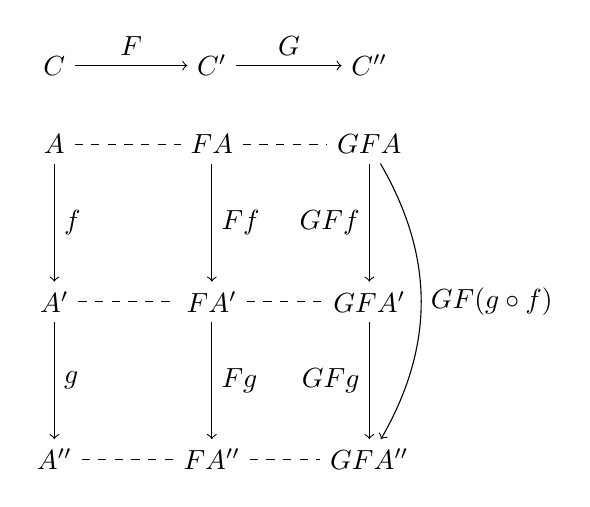
\begin{tikzpicture}[auto]
					\node (a) at (0, 2) {$A$};
					\node (a') at (0, 0) {$A'$};
					\node (a'') at (0, -2) {$A''$};
					\node (fa) at (2, 2) {$FA$};
					\node (fa') at (2, 0) {$FA'$};
					\node (fa'') at (2, -2) {$FA''$};
					\node (gfa) at (4, 2) {$GFA$};
					\node (gfa') at (4, 0) {$GFA'$};
					\node (gfa'') at (4, -2) {$GFA''$};
					\node (catc) at (0, 3) {$\cat{C}$};
					\node (catc') at (2, 3) {$\cat{C'}$};
					\node (catc'') at (4, 3) {$\cat{C''}$};
					\draw[-,dashed] (a) to (fa);
					\draw[-,dashed] (a') to (fa');
					\draw[-,dashed] (a'') to (fa'');
					\draw[-,dashed] (fa) to (gfa);
					\draw[-,dashed] (fa') to (gfa');
					\draw[-,dashed] (fa'') to (gfa'');
					\draw[->] (catc) to node{$F$}(catc');
					\draw[->] (catc') to node{$G$}(catc'');

					\draw[->] (a) to node{$f$}(a');
					\draw[->] (a') to node{$g$}(a'');

					\draw[->] (fa) to node{$Ff$}(fa');
					\draw[->] (fa') to node{$Fg$}(fa'');

					\draw[->] (gfa) to node[swap]{$GFf$}(gfa');
					\draw[->] (gfa') to node[swap]{$GFg$}(gfa'');
					\draw[->,bend left =30] (gfa) to node{$GF(g\circ f)$}(gfa'');
				\end{tikzpicture}
			\end{center}
		\end{description}
		\end{quote}
	\end{define}
	\begin{define}[恒等関手]
		任意の圏$\cat{C}$の恒等関手$\functor{Id_{\cat{C}}}{C}{C}$を以下の要素で定義する。
		\begin{quote}
			\begin{description}
				\item[対象関数] 対象関数を恒等写像$Id_{\cat{C}}(A)=A$と定義する。
				\item[射関数] 射関数を恒等写像$Id_{\cat{C}}(f)=f$と定義する。
				\item[恒等射の保存] $Id_{\cat{C}}(id_C)=id_C=id_{Id_{\cat{C}}(C)}$より恒等射を保つ
				\item[射の合成の保存] $Id_{\cat{C}}(g\circ f)=g\circ f=Id_{\cat{C}}(g)\circ Id_{\cat{C}}(f)$より射の合成を保つ。
			\end{description}
		\end{quote}
	\end{define}
	\begin{define}[小さい圏の圏]
		小さい圏の圏$\cat{Cat}$は以下の要素で構成される。

		集合の圏の時と同様に、小さい圏の「小さい」とは簡単に説明をするのであれば自己言及を防ぐための条件付けであり、実際に$\cat{Cat}$は小さい圏ではないため$\cat{Cat}$の対象にはならない。
		\begin{quote}
			\begin{description}
				\item[対象] 任意の小さい圏
				\item[射] 任意の小さい圏$\cat{A,B}$の間の任意の関手$\functor{F}{A}{B}$
				\item[射の合成] 関手$\functor{F}{C}{C'}$、$\functor{G}{C'}{C''}$に対して合成した関手$\functor{G\circ F}{C}{C'}$をとる操作を射の合成とする。
				\item[恒等射の存在]任意の圏$\cat{A}$の恒等関手$Id_{\cat{A}}$を恒等射とする。
				\item[結合律]
				$H\circ (G\circ F)=(H\circ G)\circ F$が合成可能な任意の関手$F,G,H$で成り立つことを示せばよい。
				二つの関手が等しいことを示すにはそれぞれを構成する対象関数と射関数が等しいことを示せばよい。
				対象関数については、関手$F,G,H$の対象関数$F,G,H$に対して$H\circ (G\circ F)=(H\circ G)\circ F$は明らかに成り立つ。
				射関数についても写像の結合律に還元すると、
				\begin{align*}
					(H\circ (G\circ F))_{A,A'}&=H_{GFA,GFA'}\circ (G\circ F)_{A,A}&\text{(射関数の合成の定義)}\\
					&=H_{GFA,GFA'}\circ (G_{FA,FA'}\circ F_{A,A'})&\text{(射関数の合成の定義)}\\
					&=(H_{GFA,GFA'}\circ G_{FA,FA'})\circ F_{A,A'}&\text{(写像の結合則)}\\
					&=(H\circ G)_{FA,FA'}\circ F_{A,A'}&\text{(射関数の合成の定義)}\\
					&=(H\circ (G\circ F))_{A,A'}&\text{(射関数の合成の定義)}
				\end{align*}
				となり、射関数においても結合則が成り立つ。
				\item[単位元律]
				任意の圏$\cat{C}$の恒等関手$Id_{\cat{C}}$と任意の関手$\functor{F}{X}{C}$、$\functor{G}{C}{Y}$において$Id_{\cat{C}}\circ F=F$、$G\circ Id_{\cat{C}}=G$が成り立つことを示せばよい。

				恒等関手の対象関数、射関数ともに恒等写像
				\[\mor{Id_\cat{C}=id_{\obj{A}}}{\obj{A}}{\obj{A}}\]
				\[\mor{Id_{\cat{C}A,A'}=id_{\arset{C}{A}{A'}}}{\arset{C}{A}{A'}}{\arset{C}{A}{A'}}\]
				となるため、写像の単位元律より$Id_{\cat{C}}\circ F=F$、$G\circ Id_{\cat{C}}=G$が成り立ち単位元律が成り立つ。
			\end{description}
		\end{quote}
	\end{define}
	\subsection{積圏と一点離散圏}
  一般的に圏は対象の集合や射集合を具体的な元を指定することで定義して、それが公理を満たすか確認していたが、すでに集合や写像は圏論的な操作で扱うことができる。そのため、これから$\cat{Cat}$における積対象となる積圏と、終対象となる一点離散圏、その周辺の関手を集合の圏を用いて定義していく。
	\begin{define}[積圏]
		ある圏$\cat{A,B}$に対する積圏$\cat{A\times B}$を以下の要素で定義する。
		\begin{quote}
			\begin{description}
				\item[対象] \[\obj{A\times B}=\obj{A}\times\obj{B}\]

				すなわち、圏$\cat{A}$と圏$\cat{B}$の任意の対象$A,B$の対$\tuple{A,B}$が$\cat{A\times B}$の対象であり、紛らわしくないように\[\tuple{A,B}=\pcobj{A,B}\]と表記する。

				また$\obj{A}\times\obj{B}$は直積集合であり、集合の圏の積対象であるが、対象$\pcobj{A,B}$そのものは積の普遍性を持たないことに注意してほしい。今回積とみなすのは対象ではなく圏の方である。
				\item[射]任意の対象$\pcobj{A,B},\pcobj{A',B'}$に対してその射集合をそれぞれ\[\arset{(A\times B)}{\pcobj{A,B}}{\pcobj{A',B'}}=\arset{A}{A}{A'}\times\arset{B}{B}{B'}\]と定義する。

				すなわち、圏$\cat{A}$の射$\mor{f}{A}{A'}$と圏$\cat{B}$の射$\mor{g}{B}{B'}$の元の対\[\mor{\tuple{f,g}}{[A,B]}{[A',B']}\]が$\cat{A\times B}$の射であり、対象と同様に\[\tuple{f,g}=\pcobj{f,g}\]と表記する。
				同様に$\arset{A}{A}{A'}\times\arset{B}{B}{B'}$も直積集合であり、集合の圏の積対象である。
				\begin{center}
					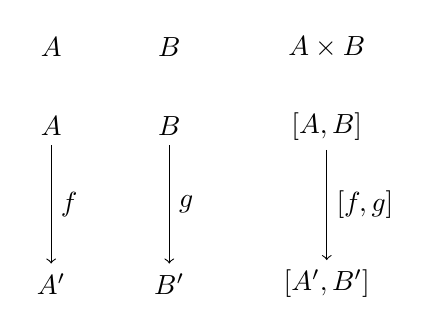
\begin{tikzpicture}[auto]
						\node (a) at (0, 0) {$A$};
						\node (a') at (0, -2) {$A'$};
						\node (b) at (1.5, 0) {$B$};
						\node (b') at (1.5, -2) {$B'$};
						\node (ab) at (3.5, 0) {$\pcobj{A,B}$};
						\node (ab') at (3.5, -2) {$\pcobj{A',B'}$};
						\draw[->] (a) to node{$f$}(a');
						\draw[->] (b) to node{$g$}(b');
						\draw[->] (ab) to node{$\pcobj{f,g}$}(ab');
						\node (cata) at (0, 1) {$\cat{A}$};
						\node (catb) at (1.5, 1) {$\cat{B}$};
						\node (catb) at (3.5, 1) {$\cat{A\times B}$};
					\end{tikzpicture}
				\end{center}
				\item[射の合成] 射$\mor{\pcobj{f,g}}{\pcobj{A,B}}{\pcobj{A',B'}}$と$\mor{\pcobj{f',g'}}{\pcobj{A',B'}}{\pcobj{A'',B''}}$の合成射\[\mor{\pcobj{f',g'}\circ\pcobj{f,g}}{\pcobj{A,B}}{\pcobj{A',B'}}\]を\[\pcobj{f',g'}\circ\pcobj{f,g}=\pcobj{f'\circ f,g'\circ g}\]と定義する。
				\begin{center}
					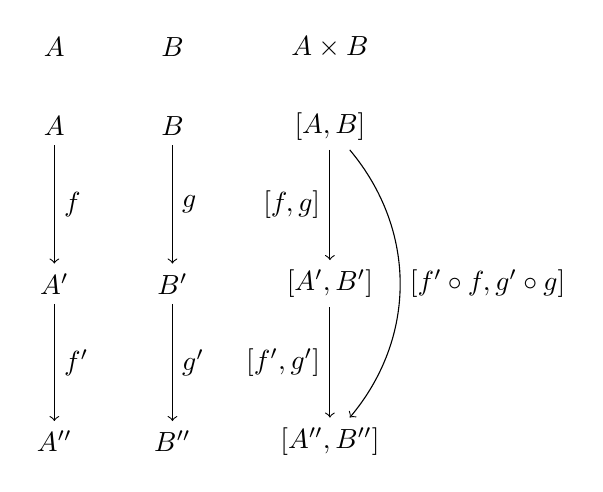
\begin{tikzpicture}[auto]
						\node (a) at (0, 0) {$A$};
						\node (a') at (0, -2) {$A'$};
						\node (a'') at (0, -4) {$A''$};
						\node (b) at (1.5, 0) {$B$};
						\node (b') at (1.5, -2) {$B'$};
						\node (b'') at (1.5, -4) {$B''$};
						\node (ab) at (3.5, 0) {$\pcobj{A,B}$};
						\node (ab') at (3.5, -2) {$\pcobj{A',B'}$};
						\node (ab'') at (3.5, -4) {$\pcobj{A'',B''}$};
						\draw[->] (a) to node{$f$}(a');
						\draw[->] (a') to node{$f'$}(a'');
						\draw[->] (b) to node{$g$}(b');
						\draw[->] (b') to node{$g'$}(b'');
						\draw[->] (ab) to node[swap]{$\pcobj{f,g}$}(ab');
						\draw[->] (ab') to node[swap]{$\pcobj{f',g'}$}(ab'');
						\draw[->,bend left =40] (ab) to node{$\pcobj{f'\circ f,g'\circ g}$}(ab'');
						\node (cata) at (0, 1) {$\cat{A}$};
						\node (catb) at (1.5, 1) {$\cat{B}$};
						\node (catb) at (3.5, 1) {$\cat{A\times B}$};
					\end{tikzpicture}
				\end{center}
				\item[恒等射の存在] 対象$[A,B]$の恒等射$id_{\pcobj{A,B}}$を\[id_{\pcobj{A,B}}=\pcobj{id_A,id_B}\]と定義する。
				\item[結合律]$(\pcobj{f'',g''}\circ\pcobj{f',g'})\circ\pcobj{f,g}=\pcobj{f'',g''}\circ(\pcobj{f',g'}\circ\pcobj{f,g})$を示せばよい。積圏の射の合成の定義を用いて圏の結合律に還元する。
				\begin{align*}
					(\pcobj{f'',g''}\circ\pcobj{f',g'})\circ\pcobj{f,g}&=\pcobj{(f''\circ f')\circ f,(g''\circ g')\circ g}&\text{(積圏の射の合成の定義)}\\
					&=\pcobj{f''\circ (f'\circ f),g''\circ (g'\circ g)}&\text{(圏$\cat{A,B}$の結合則)}\\
					&=\pcobj{f'',g''}\circ(\pcobj{f',g'}\circ\pcobj{f,g})&\text{(積圏の射の合成の定義)}
				\end{align*}
				よって成り立つ。
				\item[単位元律]任意の対象$\pcobj{A,B}$と恒等射$id_{\pcobj{A,B}}$、任意の射$\mor{\pcobj{f,g}}{\pcobj{X,Y}}{\pcobj{A,B}}$、$\mor{\pcobj{f',g'}}{\pcobj{A,B}}{\pcobj{X',Y'}}$において\[id_{\pcobj{A,B}}\circ\pcobj{f,g}=\pcobj{f,g}],\ \pcobj{f',g'}\circ id_{\pcobj{A,B}}=\pcobj{f',g'}\]が成り立つことを示せばよい。同様に積圏の射の合成の定義を用いて圏の結合律に還元する。
				\begin{align*}
					id_{\pcobj{A,B}}\circ\pcobj{f,g}&=\pcobj{id_A,id_B}\circ\pcobj{f,g}&\text{(圏$\cat{A\times B}$の恒等射の定義)}\\
					&=\pcobj{id_A\circ f,id_B\circ g}&\text{(圏$\cat{A\times B}$の射の合成の定義)}\\
					&=\pcobj{f,g}&\text{(圏$\cat{A,B}$の単位元律)}\\
					\pcobj{f',g'}\circ id_{\pcobj{A,B}}&=\pcobj{f',g'}\circ\pcobj{id_A,id_B}&\text{(圏$\cat{A\times B}$の恒等射の定義)}\\
					&=\pcobj{f'\circ id_A,g'\circ id_B}&\text{(圏$\cat{A\times B}$の射の合成の定義)}\\
					&=\pcobj{f',g'}&\text{(圏$\cat{A,B}$の単位元律)}
				\end{align*}
				よって単位元律が成り立つ。
			\end{description}
		\end{quote}
	\end{define}


	\begin{define}[射影関手]
		関手$\functor{\Pi_{L,\cat{A\times B}}}{A\times B}{A}$を以下の写像で定義する。また射影射と同様に紛らわしくない場合に$\Pi_{L,\cat{A\times B}}=\Pi_\cat{A}$と表記する。
		\begin{quote}
			\begin{description}
				\item[対象関数] 積圏の対象の定義より、圏$\cat{A\times B}$の対象の集合は$\obj{A}\times\obj{B}$である。これを集合の圏における積とみなし、射影写像\[\mor{\Pi_\cat{A}=\pi_{\obj{A}}}{\obj{A}\times\obj{B}}{\obj{A}}\]を対象関数とする。
				すなわち$\Pi_\cat{A}(\pcobj{A,B})=A$となるような写像である。
				\item[射関数] 対象関数と同様に射集合$\arset{A}{A}{A'}\times\arset{B}{B}{B'}$の射影写像\[\mor{\Pi_\cat{A}=\pi_{\arset{A}{A}{A'}}}{\arset{A}{A}{A'}\times\arset{B}{B}{B'}}{\arset{A}{A}{A'}}\]を射関数とする。
				すなわち$\Pi_\cat{A}(\pcobj{f,g})=f$となるような写像である。
				\item[恒等射の保存] $\Pi_\cat{A}(id_{A\times B})=\Pi_\cat{A}(\pcobj{id_A,id_B})=id_A$より恒等射を保つ
				\item[射の合成の保存]元の圏の結合則に還元する。
				\begin{align*}
					\Pi_\cat{A}(\pcobj{f',g'}\circ\pcobj{f,g})&=\Pi_\cat{A}(\pcobj{f'\circ f, g'\circ g})&\text{($\cat{A\times B}$の射の合成の定義)}\\
					&=f'\circ f&\text{(射関数の定義)}\\
					&=\Pi_\cat{A}(\pcobj{f',g'})\circ\Pi_A(\pcobj{f,g})&\text{(射関数の定義)}
				\end{align*}
				よって射の合成を保つ。
			\end{description}
		\end{quote}
	\end{define}
	また同様に$\functor{\Pi_{R,\cat{A\times B}}}{A\times B}{B}$も定義できる。
	\begin{define}[関手の対]
		関手$\functor{F}{X}{A}$と$\functor{G}{X}{B}$の対$\functor{\tuple{F,G}}{X}{A\times B}$を以下の写像で定義する。
		\begin{quote}
			\begin{description}
				\item[対象関数] 関手$F,G$の対象関数$\mor{F}{\obj{X}}{\obj{A}}$、$\mor{G}{\obj{X}}{\obj{B}}$の対
				\begin{align*}
					&\mor{\tuple{F,G}}{\obj{X}}{\obj{A\times B}}\\
					=&\mor{\tuple{F,G}}{\obj{X}}{\obj{A}\times \obj{B}}
				\end{align*}
				を対象関数とする。
				すなわち圏$\cat{X}$の対象$X$に対して$\tuple{F,G}(X)=\pcobj{FX,GX}$となるような写像である。
				\item[射関数]
				関手$F,G$の対象$X,X'$に対する射関数$\mor{F_{X,X'}}{\arset{X}{X}{X'}}{\arset{A}{FX}{FX'}},\ \mor{G_{X,X'}}{\arset{X}{X}{X'}}{\arset{B}{GX}{GX'}}$の対
				\begin{align*}
					&\mor{\tuple{F,G}_{X,X'}&&}{\arset{X}{X}{X'}}{\arset{A\times B}{\tuple{FX,GX}}{\tuple{FX',GX'}}}\\
					=&	\mor{\tuple{F_{X,X'},G_{X,X'}}&&}{\arset{X}{X}{X'}}{\arset{A}{FX}{FX'}\times\arset{B}{GX}{GX'}}
				\end{align*}
				を射関数とする。
				すなわち射$\mor{f}{X}{X'}$に対して\[\mor{\tuple{F,G}(f)=\pcobj{Ff,Gf}}{\pcobj{FX,GX}}{\pcobj{FX',GX'}}\]となるような写像である。

				\begin{center}
					\begin{tikzpicture}[auto]
						\node (x) at (-1.5, 0) {$X$};
						\node (x') at (-1.5, -2) {$X'$};
						\node (a) at (0, 0) {$FX$};
						\node (a') at (0, -2) {$FX'$};
						\node (b) at (1.5, 0) {$GX$};
						\node (b') at (1.5, -2) {$GX'$};
						\node (ab) at (3.5, 0) {$[FX,GX]$};
						\node (ab') at (3.5, -2) {$[FX',GX']$};
						\draw[->] (x) to node{$f$}(x');
						\draw[->] (a) to node{$Ff$}(a');
						\draw[->] (b) to node{$Gf$}(b');
						\draw[->] (ab) to node{$[Ff,Gf]$}(ab');
						\node (cata) at (-1.5, 1) {$\cat{X}$};
						\node (cata) at (0, 1) {$\cat{A}$};
						\node (catb) at (1.5, 1) {$\cat{B}$};
						\node (catb) at (3.5, 1) {$\cat{A\times B}$};
					\end{tikzpicture}
				\end{center}
				\item[恒等射の保存]
				\begin{align*}
					\tuple{F,G}(id_X)&=\pcobj{F(id_X),G(id_X)}&\text{(射関数の定義)}\\
					&=\pcobj{id_{FX},id_{GX}}&\text{($F,G$の恒等射の保存)}\\
					&=id_{\pcobj{FX,GX}}&\text{(積圏の恒等射の定義)}
				\end{align*}
			よって恒等射を保つ
				\item[射の合成の保存]
				\begin{align*}
					\tuple{F,G}(f'\circ f)&=\pcobj{F(f'\circ f),G(f'\circ f)}&\text{(射関数の定義)}\\
					&=\pcobj{Ff'\circ Ff, Gf'\circ Gf}&\text{($F,G$の射の合成の保存)}\\
					&=\pcobj{Ff',Gf'}\circ\pcobj{Ff,Gf}&\text{(積圏の射の合成の定義)}\\
					&=\tuple{F,G}(f')\circ\tuple{F,G}(f)&\text{(射関数の定義)}
				\end{align*}
			よって射の合成を保つ。
			\end{description}
		\end{quote}
	\end{define}
	\begin{prop}
		積圏$\cat{A\times B}$と射影関手$\Pi_\cat{A},\Pi_\cat{B}$の組$(\cat{A\times B},\Pi_\cat{A},\Pi_\cat{B})$は$\cat{Cat}$における積である。
	\end{prop}
	\begin{proof}
		積$(\cat{A\times B},\Pi_\cat{A},\Pi_\cat{B})$において、圏$\cat{X}$、関手$\functor{F}{X}{A}$、$\functor{G}{X}{B}$で構成される任意の組$(\cat{X},F,G)$に対して、$\Pi_\cat{A}\circ\tuple{F,G}=F,\ \Pi_\cat{B}\circ\tuple{F,G}=G$が成り立つような関手の対$\functor{\tuple{F,G}}{X}{A\times B}$が一意に存在することを示せばよい。
		\begin{center}
			\begin{tikzpicture}[auto]
				\node (a) at (0, 0) {$\cat{A}$};
				\node (ab) at (2, 0) {$\cat{A\times B}$};
				\node (b) at (4, 0) {$\cat{B}$};
				\node (x) at (2, 2) {$\cat{X}$};
				\draw[->] (x) to node[swap]{$F$}(a);
				\draw[->] (x) to node{$G$}(b);
				\draw[->] (ab) to node{$\Pi_\cat{A}$}(a);
				\draw[->] (ab) to node[swap]{$\Pi_\cat{B}$}(b);
				\draw[->] (x) to node{$\tuple{F,G}$}(ab);
			\end{tikzpicture}
		\end{center}
		端的に述べるなら積圏、関手の対、射影関手の各々が持つ対象関数、射関数はそれぞれ積対象、射の対、射影射で構成されることから、積の普遍性を満たすことを示すのは難しくない。

		関手$F,G$の対象関数$F,G$、射影関手$\Pi_\cat{A},\Pi_\cat{B}$の対象関数$\pi_{\obj{A}},\pi_{\obj{B}}$、そして関手の対の対象関数$\tuple{F,G}$は、その定義により積の図式となる。
		すなわち対象関数$F,G$に対して対象関数$\tuple{F,G}$は一意に存在する。
		\begin{center}
			\begin{tikzpicture}[auto]
				\node (a) at (0, 0) {$\obj{A}$};
				\node (ab) at (4, 0) {$\obj{A}\times\obj{B}$};
				\node (abp) at (4, -1) {$\obj{A\times B}$};
				\node (b) at (8, 0) {$\obj{B}$};
				\node (x) at (4, 2) {$\obj{X}$};
				\draw[double distance=2pt] (ab) to (abp);
				\draw[->] (x) to node[swap]{$F$}(a);
				\draw[->] (x) to node{$G$}(b);
				\draw[->] (ab) to node{$\pi_{\obj{A}}$}(a);
				\draw[->] (ab) to node[swap]{$\pi_{\obj{B}}$}(b);
				\draw[->] (x) to node{$\tuple{F,G}$}(ab);
			\end{tikzpicture}
		\end{center}
		各射関数による積の図式は省略するが、同様に射関数$\tuple{F,G}$が一意に存在することが分かる。よって可換性を満たす対象関数と射関数も一意に存在することから、関手の対は積圏における射の対となり、$(\cat{A\times B},\Pi_\cat{A},\Pi_\cat{B})$は積の普遍性を満たす。
	\end{proof}
	\begin{define}[一点離散圏]
	一つの対象と一つの恒等射で構成される圏$\cat{1}$を一点離散圏とよぶ。
	\end{define}
	\begin{prop}[$\cat{Cat}$の終対象]
		$\cat{1}$は$\cat{Cat}$における終対象である。
	\end{prop}
	\begin{proof}
		任意の圏$\cat{C}$から一点離散圏$\cat{1}$への関手$!_{\cat{C}}$を考える。
		まず$\cat{1}$の対象$*$と射$id_*$は一つしか存在しない。そのため一点集合を$1$として
		\[\obj{1}=1,\ \arset{1}{*}{*}=1\]が成り立つ。

		よって対象関数$!_{\cat{C}}$は
		\begin{align*}
			&\mor{!_{\cat{C}}}{\obj{C}}{\obj{1}}\\
			=&\mor{!_{\cat{C}}}{\obj{C}}{1}
		\end{align*}
		となり一点集合への写像であることがわかる。よって任意の対象$A$に対して$!_{\cat{C}}(A)=*$が成り立ち、このような対象関数が一意に存在することが分かった。

		また任意の二対象$A,B$に対する射関数は
		\begin{align*}
			&\mor{{!_{\cat{C}}}_{A,B}}{\arset{C}{A}{B}}{\arset{1}{!_{\cat{C}}(A)}{!_{\cat{C}}(B)}}\\
			=&\mor{{!_{\cat{C}}}_{A,B}}{\arset{C}{A}{B}}{\arset{1}{*}{*}}\\
			=&\mor{{!_{\cat{C}}}_{A,B}}{\arset{C}{A}{B}}{1}\\
		\end{align*}と書ける。
		よって二対象$A,B$に対する各射関数も一意に存在することが分かった。

		関手$!_{\cat{C}}$の二つの写像が圏$\cat{C}$に対して一意に存在することわかる。
		よって任意の圏$\cat{C}$から一点離散圏$\cat{1}$への関手は一意に存在するから、一点離散圏$\cat{1}$は$\cat{Cat}$における終対象であることが示せた。
	\end{proof}
	\begin{prop}[圏における元]
		任意の圏$\cat{C}$の元、つまり関手$\functor{A}{1}{C}$は圏$\cat{C}$の対象とみなせる。
	\end{prop}
	\begin{proof}
		関手$\functor{A}{1}{C}$は対象関数$\mor{F}{\obj{1}}{\obj{C}}$、射関数$\mor{F}{\arset{1}{*}{*}}{\arset{C}{F(*)}{F(*)}}$で構成される。このとき、$\obj{1}$は一点集合であるから、対象関数$F$は$\obj{C}$の元である。

		また射関数も同様に$\arset{C}{F(*)}{F(*)}$の元であるが、恒等射の保存より写される射は恒等射ただ一つであり、射関数は対象関数に対して一通りにしか定義できないから考慮しなくてもよい。

		よって関手$\functor{A}{1}{C}$は圏$\cat{C}$の対象とみなせる。
	\end{proof}
	積圏$\cat{A\times B}$の対象を$\pcobj{A,B}$と表したが、実際に対象$\functor{A}{1}{A}$と対象$\functor{B}{1}{B}$の関手の対$\functor{\tuple{A,B}}{1}{A\times B}$は$\cat{A\times B}$の対象になる。

	\subsection{特殊な関手}
	対象や射を二つ取るような2変数関数のような関手について考える。
	\begin{define}[双関手]
		積圏からの関手、つまり$\functor{F}{A\times B}{C}$となるような関手を双関手とする。

		また積圏の任意の対象$[A,B]$に対し、\[F(\pcobj{A,B})=F(A,B)\]と略記する。
		さらに積圏の射$\mor{\pcobj{f,id_B}}{\pcobj{A,B}}{\pcobj{A,B'}}$において\[F(\pcobj{f,id_B})=F(f,B)\]と表記する。
	\end{define}
	圏$\cat{A}$の射$f$と圏$\cat{B}$の射$g$がどのように圏$\cat{C}$に写されるのかを以下の可換図式で確認してほしい。
	\begin{center}
		\begin{tikzpicture}[auto]
			\node (a) at (0, 0) {$A$};
			\node (a') at (0, -2.5) {$A'$};
			\node (b) at (2, 1) {$B$};
			\node (b') at (4.5, 1) {$B'$};
			\node (ab) at (2, 0) {$\pcobj{A,B}$};
			\node (a'b) at (2, -2.5) {$\pcobj{A',B}$};
			\node (ab') at (4.5, 0) {$\pcobj{A,B}$};
			\node (a'b') at (4.5, -2.5) {$\pcobj{A',B'}$};

			\node (fab) at (8, 0) {$F(A,B)$};
			\node (fa'b) at (8, -2.5) {$F(A',B)$};
			\node (fab') at (10.5, 0) {$F(A,B')$};
			\node (fa'b') at (10.5, -2.5) {$F(A',B')$};

			\node (cata) at (-1, -1.25) {$\cat{A}$};
			\node (catb) at (3.25, 2) {$\cat{B}$};
			\node (catab) at (3.25, -3.5) {$\cat{A\times B}$};
			\node (catc) at (9.25, -3.5) {$\cat{C}$};

			\draw[->] (a) to node[swap]{$f$}(a');
			\draw[->] (b) to node{$g$}(b');
			\draw[->] (ab) to node[swap]{$\pcobj{f,id_B}$}(a'b);
			\draw[->] (ab') to node{$\pcobj{f,id_{B'}}$}(a'b');
			\draw[->] (ab) to node{$\pcobj{id_A,g}$}(ab');
			\draw[->] (a'b) to node[swap]{$\pcobj{id_{A'},g}$}(a'b');
			\draw[->] (ab) to node{$\pcobj{f,g}$}(a'b');

			\draw[->] (fab) to node[swap]{$F(f,B)$}(fa'b);
			\draw[->] (fab') to node{$F(f,B')$}(fa'b');
			\draw[->] (fab) to node{$F(A,g)$}(fab');
			\draw[->] (fa'b) to node[swap]{$F(A',g)$}(fa'b');
			\draw[->] (fab) to node{$F(f,g)$}(fa'b');
			\draw[->] (catab) to node{$F$}(catc);
		\end{tikzpicture}
	\end{center}
	次に双関手の例として積関手$\functor{-\times B}{C}{C}$を双関手に拡張しようと思う。
	\begin{define}[双積関手]
		積を持つ圏$\cat{C}$上の双積関手$\functor{-\times -}{C\times C}{C}$を以下の写像で定義する。
		\begin{quote}
			\begin{description}
				\item[対象関数] 対象関数を積圏$\cat{C\times C}$の任意の対象$\pcobj{A,B}$に対して\[(-\times -)(A,B)=A\times B\]と定義する。
				\item[射関数] 二対象$\pcobj{A,B},\pcobj{A',B'}$に対する射関数を任意の射$\mor{\pcobj{f,g}}{\pcobj{A,B}}{\pcobj{A',B'}}$に対して\[(-\times -)_{\pcobj{A,B},\pcobj{A',B'}}(f,g)=f\times g\]と定義する。
				\begin{center}
					\begin{tikzpicture}[auto]
						\node (ab) at (0, 0) {$\pcobj{A,B}$};
						\node (a'b') at (0, -2) {$\pcobj{A',B'}$};
						\node (pab) at (3, 0) {$A\times B$};
						\node (pa'b') at (3, -2) {$A'\times B'$};
						\node (catcc) at (0, 1) {$\cat{C\times C}$};
						\node (catc) at (3, 1) {$\cat{C}$};
						\draw[-,dashed] (ab) to (pab);
						\draw[-,dashed] (a'b') to (pa'b');
						\draw[->] (ab) to node{$\pcobj{f,g}$}(a'b');
						\draw[->] (pab) to node{$f\times g$}(pa'b');
						\draw[->] (catcc) to node{$(-\times-)$}(catc);
					\end{tikzpicture}
				\end{center}

				\item[恒等射の保存] $(-\times -)(id_{\pcobj{A,B}})=id_{(-\times-)(A,B)}$を示せばよい。
				\begin{align*}
					(-\times -)(id_{\pcobj{A,B}})&=id_A\times id_B&\text{(射関数の定義)}\\
					&=\pcobj{id_A\circ\pi_A,id_B\circ\pi_B}&\text{(射の積の定義)}\\
					&=id_{A\times B}&\text{(射影射の対)}\\
					&=id_{(-\times-)(A,B)}&\text{(対象関数の定義)}
				\end{align*}
				よって恒等射を保つ。
				\item[射の合成の保存] $(-\times -)(f',g')\circ(-\times-)(f,g)=(-\times-)(\pcobj{f',g'}\circ\pcobj{f,g}$を示せばよい。
				\begin{align*}
					(-\times -)(f',g')\circ(-\times-)(f,g)&=(f'\times g')\circ(f\times g)&\text{(射関数の定義)}\\
					&=(f'\circ f)\times(g'\circ g)&\text{(積と合成の交換)}\\
					&=(-\times-)(f'\circ f,g'\circ g)&\text{(射関数の定義)}\\
					&=(-\times-)(\pcobj{f'\circ f,g'\circ g})\\
					&=(-\times-)(\pcobj{f',g'}\circ\pcobj{f,g})&\text{(積圏の射の合成の定義)}
				\end{align*}
				よって射の合成を保つ。
			\end{description}
		\end{quote}
	\end{define}
	対象の積と圏の積が紛らわしいが、まず圏の積の対象$\pcobj{A,B}$は圏$\cat{C}$の$A$と$B$の積が存在しなくとも定義することができ、その点で対象の積$A\times B$より一般的な概念だと考えられる。よってイメージとしては圏$\cat{C}$の外側$\cat{C\times C}$で定義した対象の積もどき$[A,B]$を圏$\cat{C}$に挿入する操作が関手$(-\times-)$と考えられる。ただし、双積関手で写された対象が積の普遍性を満たすかどうかは現段階では説明できない。

	また以前に圏$\cat{C}$の射の積と積圏$\cat{C\times C}$の射の振る舞いが似ていることについて述べたが、実際に関手として二つの射の関係性を示すことができた。
	\begin{define}[双対圏]
		ある圏$\cat{C}$に対する双対圏$\cat{C}^{op}$を以下の要素で定義する。
		\begin{quote}
			\begin{description}
				\item[対象] $\obj{C^{op}}=\obj{C}$とする。

				また圏$\cat{C}$の対象$A$に対応する双対圏$\cat{C^{op}}$の対象も$A$であるが、$\cat{C^{op}}$の対象は$A^{op}$として表記上区別する。
				\item[射] 任意の二対象$A^{op}, B^{op}$に対して射集合を\[\arset{C^{op}}{B^{op}}{A^{op}}=\arset{C}{A}{B}\]と定義する。
				同様に射$\mor{f}{A}{B}$に対応する射を表記上$\mor{f^{op}}{B^{op}}{A^{op}}$とする。
				圏$\cat{C}$と双対圏$\cat{C^{op}}$では射の向きが入れ替わっていることに注意してほしい。
				\begin{center}
					\begin{tikzpicture}[auto]
						\node (a) at (0, 0) {$A$};
						\node (b) at (0, -1.5) {$B$};
						\node (fa) at (1.5, 0) {$A^{op}$};
						\node (fb) at (1.5, -1.5) {$B^{op}$};
						\node (catc) at (0, 1) {$\cat{C}$};
						\node (catd) at (1.5, 1) {$\cat{C^{op}}$};
						\draw[->] (a) to node{$f$}(b);
						\draw[->] (fb) to node{$f^{op}$}(fa);
					\end{tikzpicture}
				\end{center}
				\item[射の合成] 圏$\cat{C}$の射$\mor{f}{A}{B}$、$\mor{g}{B}{C}$の合成射$\mor{g\circ f}{A}{C}$に対して、双対圏$\cat{C}^{op}$の射$\mor{f^{op}}{B^{op}}{A^{op}}$、$\mor{g^{op}}{C^{op}}{B^{op}}$の合成射を
				\[\mor{(g\circ f)^{op}=f^{op}\circ g^{op}}{C^{op}}{A^{op}}\]
				と定義する。
				圏$\cat{C}$と$\cat{C}^{op}$では射の合成の順序が入れ替わっていることに注意してほしい。
				\begin{center}
					\begin{tikzpicture}[auto]
						\node (a) at (0, 0) {$A$};
						\node (b) at (1.5, -1) {$B$};
						\node (c) at (0, -2) {$C$};
						\node (fa) at (4, 0) {$A^{op}$};
						\node (fb) at (5.5, -1) {$B^{op}$};
						\node (fc) at (4, -2) {$C^{op}$};
						\node (catc) at (0.75, 1) {$\cat{C}$};
						\node (catd) at (4.75, 1) {$\cat{C^{op}}$};
						\draw[->] (a) to node{$f$}(b);
						\draw[->] (b) to node{$g$}(c);
						\draw[->] (a) to node[swap]{$g\circ f$}(c);
						\draw[->] (fb) to node[swap]{$f^{op}$}(fa);
						\draw[->] (fc) to node[swap]{$g^{op}$}(fb);
						\draw[->] (fc) to node{$(g\circ f)^{op}$}(fa);
					\end{tikzpicture}
				\end{center}
				\item[恒等射の存在]圏$\cat{C}$の任意の恒等射$\mor{id_A}{A}{A}$に対して、双対圏$\cat{C}^{op}$の恒等射を\[\mor{(id_A)^{op}=id_{A^{op}}}{A^{op}}{A^{op}}\]と定義する。
				\item[結合律] 合成可能な任意の射$f^{op},g^{op},h^{op}$において、
				\begin{align*}
					(f^{op}\circ g^{op})\circ h^{op}&=(g\circ f)^{op}\circ h^{op}\\
					&=(h\circ(g\circ f))^{op}\\
					&=((h\circ g)\circ f)^{op}\\
					&=f^{op}\circ (h\circ g)^{op}\\
					&=f^{op}\circ (g^{op}\circ h^{op})
				\end{align*}
				となるので結合律を満たす。
				\item[単位元律]任意の恒等射$id_{A^{op}}$、任意の射$\mor{f^{op}}{X^{op}}{A^{op}}$、$\mor{g^{op}}{A^{op}}{Y^{op}}$に対し$id_{A^{op}}\circ f^{op}=f^{op}$、$g^{op}\circ id_{A^{op}}=g^{op}$を示せばよい。
				\begin{align*}
					id_{A^{op}}\circ f^{op}&={id_A}^{op}\circ f^{op}&\text{(双対圏の恒等射の定義)}\\
					&=(f\circ id_A)^{op}&\text{(双対圏の射の合成の定義)}\\
					&=f^{op}&\text{(単位元律)}\\
					g^{op}\circ id_{A^{op}}&=g^{op}\circ {id_A}^{op}&\text{(双対圏の恒等射の定義)}\\
					&=(id_A\circ g)^{op}&\text{(双対圏の射の合成の定義)}\\
					&=g^{op}&\text{(単位元律)}\\
				\end{align*}
				よって単位元律を見たす。
			\end{description}
		\end{quote}
	\end{define}
	
	\begin{define}[双対関手]
		ある圏$\cat{C,D}$に対する双対圏$\cat{C}^{op},\cat{D}^{op}$と関手$\functor{F}{C}{D}$に対して、双対関手$\functor{F^{op}}{C^{op}}{D^{op}}$を以下の要素で定義する。
		\begin{quote}
			\begin{description}
				\item[対象関数]対象関数$\mor{F^{op}}{C^{op}}{D^{op}}$を任意の対象$A^{op}$に対して
				\[F^{op}(A^{op})=(FA)^{op}\]と定義する。
				
				\item[射関数]対象関数と同様に、射関数\[\mor{{F^{op}}_{A^{op},B^{op}}}{\arset{C^{op}}{A^{op}}{B^{op}}}{\arset{D^{op}}{(FA)^{op}}{(FB)^{op}}}\]を任意の射$\mor{f}{A^{op}}{B^{op}}$に対して
				\[F^{op}(f^{op})=(Ff)^{op}\]と定義する。

				\begin{center}
					\begin{tikzpicture}[auto]
						\node (a) at (0, 0) {$A^{op}$};
						\node (b) at (0, -1.5) {$B^{op}$};
						\node (fa) at (1.5, 0) {$(FA)^{op}$};
						\node (fb) at (1.5, -1.5) {$(FB)^{op}$};
						\node (catc) at (0, 1) {$\cat{C^{op}}$};
						\node (catd) at (1.5, 1) {$\cat{D^{op}}$};
						\draw[-,dashed] (a) to (fa);
						\draw[-,dashed] (b) to (fb);
						\draw[->] (b) to node{$f^{op}$}(a);
						\draw[->] (fb) to node[swap]{$(Ff)^{op}$}(fa);
						\draw[->] (catc) to node{$F^{op}$}(catd);
					\end{tikzpicture}
					\begin{tikzpicture}[auto]
						\node (a) at (0, 0) {$A$};
						\node (b) at (0, -1.5) {$B$};
						\node (fa) at (1.5, 0) {$FA$};
						\node (fb) at (1.5, -1.5) {$FB$};
						\node (catc) at (0, 1) {$\cat{C}$};
						\node (catd) at (1.5, 1) {$\cat{D}$};
						\draw[-,dashed] (a) to (fa);
						\draw[-,dashed] (b) to (fb);
						\draw[->] (a) to node{$f$}(b);
						\draw[->] (fa) to node{$Ff$}(fb);
						\draw[->] (catc) to node{$F$}(catd);
					\end{tikzpicture}
				\end{center}
				\item[恒等射の保存]元の関手$F$の恒等射の保存に還元して$F^{op}(id_{A^{op}})=id_{(FA)^{op}}$を示す
				\begin{align*}
					F^{op}(id_{A^{op}})&=F^{op}(id_A)^{op}&\text{(双対圏の恒等射の定義)}\\
					&=(F(id_A))^{op}&\text{双対関手の射関数の定義}\\
					&=(id_{FA})^{op}&\text{$F$の恒等者の保存}\\
					&=id_{(FA)^{op}}&\text{(双対圏の恒等射の定義)}
				\end{align*}
				
				\item[射の合成の保存]同様に元の関手の合成の保存に還元して\[F^{op}(f^{op}\circ g^{op})=F^{op}f^{op}\circ F^{op}g^{op}\]を示す。
				\begin{align*}
					F^{op}(f^{op}\circ g^{op})&= F^{op}(g\circ f)^{op}&\text{(双対圏の射の合成)}\\
					&=(F(g\circ f))^{op}&\text{(双対関手の射関数の定義)}\\
					&=(Fg\circ Ff)^{op}&\text{($F$の射の合成の保存)}\\
					&=(Fg)^{op}\circ (Ff)^{op}&\text{(双対圏の射の合成)}\\
					&=F^{op}f^{op}\circ F^{op}g^{op}&\text{(双対関手の射関数の定義)}
				\end{align*}
			\end{description}
		\end{quote}
	\end{define}

	双対関手では反転した射を反転したまま写した。次に定義する反変関手では通常の射を反転した射に写すような操作を考える。
	\begin{define}[反変関手]
		圏$\cat{C}$から圏$\cat{D}$への反変関手と呼ばれる圏の間の写像$\functor{F}{C}{D}$を以下の写像と公理で定義する。
		\begin{quote}
			\begin{description}
				\item[対象関数] $\cat{C}$の対象$A$に$\cat{D}$の対象$FA$を割り当てる対象関数\[\mor{F}{\obj{C}}{\obj{D}}\]
				これは通常の関手と同じである。
				\item[射関数] $\cat{C}$の任意の各対象$A,B$において射$\mor{f}{A}{B}$に圏$\cat{D}$の射$\mor{Ff}{FB}{FA}$を割り当てる射関数\[\mor{F_{A,B}}{\arset{C}{A}{B}}{\arset{D}{FB}{FA}}\]これも同様に対象$A,B$に対してそれぞれ存在する射関数$F_{A,B}$を総称して$F$と呼ぶことにする。				
				\begin{center}
					\begin{tikzpicture}[auto]
						\node (a) at (0, 0) {$A$};
						\node (b) at (0, -1.5) {$B$};
						\node (fa) at (1.5, 0) {$FA$};
						\node (fb) at (1.5, -1.5) {$FB$};
						\node (catc) at (0, 1) {$\cat{C}$};
						\node (catd) at (1.5, 1) {$\cat{D}$};
						\draw[-,dashed] (a) to (fa);
						\draw[-,dashed] (b) to (fb);
						\draw[->] (a) to node{$f$}(b);
						\draw[->] (fb) to node{$Ff$}(fa);
						\draw[->] (catc) to node{$F$}(catd);
					\end{tikzpicture}
				\end{center}
				双対圏を取る操作と同じように、射を写すときは射の向きを逆にする。
				\item[恒等射の保存] $F(id_A)=id_{FA}$が任意の恒等射で成り立つ。
				\item[射の合成の保存] 合成可能な任意の二射$f,g$において\[F(g\circ f)=Ff\circ Fg\]が成り立つ。

				\begin{center}
					\begin{tikzpicture}[auto]
						\node (a) at (0, 0) {$A$};
						\node (b) at (0, -1.5) {$B$};
						\node (c) at (0, -3) {$C$};
						\node (fa) at (1.5, 0) {$FA$};
						\node (fb) at (1.5, -1.5) {$FB$};
						\node (fc) at (1.5, -3) {$FC$};
						\node (catc) at (0, 1) {$\cat{C}$};
						\node (catd) at (1.5, 1) {$\cat{D}$};
						\draw[-,dashed] (a) to (fa);
						\draw[-,dashed] (b) to (fb);
						\draw[-,dashed] (c) to (fc);
						\draw[->] (a) to node{$f$}(b);
						\draw[->] (b) to node{$g$}(c);
						\draw[->] (fb) to node{$Ff$}(fa);
						\draw[->] (fc) to node{$Fg$}(fb);
						\draw[->,bend right = 30] (fc) to node[swap]{$F(g\circ f)=Ff\circ Fg$}(fa);
						\draw[->] (catc) to node{$F$}(catd);
					\end{tikzpicture}
				\end{center}
				双対圏の射の合成と同じように、合成射を写すときは合成の順序を逆にして写す。
			\end{description}
		\end{quote}
	\end{define}
	この反変関手は関手とついているが、双対関手とは違い以前定義した関手の性質を満たさず、関手とはならない。そのため区別が必要な場合、一般の関手を共変関手と呼ぶことにする。
	また反変関手$\functor{F}{C}{D}$は共変関手$\functor{F}{C^{op}}{D}$とみなせる。
		\begin{center}
			\begin{tikzpicture}[auto]
				\node (a) at (0, 0) {$A$};
				\node (b) at (0, -1.5) {$B$};
				\node (fa) at (1.5, 0) {$FA$};
				\node (fb) at (1.5, -1.5) {$FB$};
				\node (catc) at (0, 1) {$\cat{C}$};
				\node (catd) at (1.5, 1) {$\cat{D}$};
				\draw[-,dashed] (a) to (fa);
				\draw[-,dashed] (b) to (fb);
				\draw[->] (a) to node{$f$}(b);
				\draw[->] (fb) to node{$Ff$}(fa);
				\draw[->] (catc) to node{$F$}(catd);

				\node (a) at (3.5, 0) {$A$};
				\node (b) at (3.5, -1.5) {$B$};
				\node (aop) at (5, 0) {$A^{op}$};
				\node (bop) at (5, -1.5) {$B^{op}$};
				\node (fa) at (6.5, 0) {$FA$};
				\node (fb) at (6.5, -1.5) {$FB$};
				\node (catcop) at (3.5, 1) {$\cat{C}$};
				\node (catc) at (5, 1) {$\cat{C^{op}}$};
				\node (catd) at (6.5, 1) {$\cat{D}$};
				\draw[-,dashed] (aop) to (fa);
				\draw[-,dashed] (bop) to (fb);
				\draw[->] (bop) to node{$f^{op}$}(aop);
				\draw[->] (a) to node{$f$}(b);
				\draw[->] (fb) to node{$Ff$}(fa);
				\draw[->] (catc) to node{$F$}(catd);
			\end{tikzpicture}
		\end{center}
	\subsection{Hom関手}
  圏$\cat{C}$の対象$A,B$に対して射集合$\arset{C}{A}{B}$や射写像$\arset{C}{A}{f}$を考えることができたが、これらも圏$\cat{C}$の対象、射によって添字付けられた集合、射と考えることで、関手として定式化することができる。
  そのためにもまずは改めてこれらの写像の性質を確認していこうと思う。

	\begin{prop}[共変射写像の恒等射の保存]
		圏$\cat{C}$の任意の対象$X,A$において
		\[\arset{C}{X}{id_A}=id_{\arset{C}{X}{A}}\]が成り立つ。
		\begin{center}
			\begin{tikzpicture}[auto]
				\node (x) at (-1.5, 0) {$X$};
				\node (x2) at (-1.5, -1.5) {$X$};
				\node (a) at (0, 0) {$A$};
				\node (b) at (0, -1.5) {$A$};
				\node (ca) at (2, 0) {$\arset{C}{X}{A}$};
				\node (cb) at (2, -1.5) {$\arset{C}{X}{A}$};
				\node (catc) at (-0.75, 1) {$\cat{C}$};
				\node (catc) at (2, 1) {$\cat{Set}$};
				\draw[->] (ca) to node{$\arset{C}{X}{id_A}$}(cb);
				\draw[->] (a) to node{$id_A$}(b);
				\draw[double distance=2pt] (x) to (x2);
				\draw[->] (x) to node{$g$}(a);
				\draw[->] (x2) to node[swap]{$g$}(b);
			\end{tikzpicture}
		\end{center}
	\end{prop}
	\begin{proof}
		任意の射$\mor{g}{X}{A}$に対して
		\begin{align*}
			\arset{C}{X}{id_A}(g)&=id_A\circ g&\text{(共変射写像の定義)}\\
			&=g&\text{(単位元律)}\\
			&=id_{\arset{C}{X}{A}}(g)&\text{($\cat{Set}$の恒等射の定義)}\\
		\end{align*}
		よって$\arset{C}{X}{id_A}=id_{\arset{C}{X}{A}}$が成り立つ。
	\end{proof}
	\begin{prop}[共変射写像の合成の保存]
		圏$\cat{C}$の任意の対象$X,A,B,C$と射$\mor{f}{A}{B}$、$\mor{g}{B}{C}$、$\mor{h}{X}{A}$に対して、
		\[\arset{C}{X}{g\circ f}=\arset{C}{X}{g}\circ\arset{C}{X}{f}\]が成り立つ。
		\begin{center}
			\begin{tikzpicture}[auto]
				\node (x) at (-1.5, 0) {$X$};
				\node (x2) at (-1.5, -1.5) {$X$};
				\node (x3) at (-1.5, -3) {$X$};
				\node (a) at (0, 0) {$A$};
				\node (b) at (0, -1.5) {$B$};
				\node (c) at (0, -3) {$C$};
				\node (ca) at (2, 0) {$\arset{C}{X}{A}$};
				\node (cb) at (2, -1.5) {$\arset{C}{X}{B}$};
				\node (cc) at (2, -3) {$\arset{C}{X}{C}$};
				\node (catc) at (-0.75, 1) {$\cat{C}$};
				\node (catc) at (2, 1) {$\cat{Set}$};
				\draw[->] (ca) to node{$\arset{C}{X}{f}$}(cb);
				\draw[->] (cb) to node{$\arset{C}{X}{g}$}(cc);
				\draw[->] (a) to node{$f$}(b);
				\draw[->] (b) to node{$g$}(c);
				\draw[double distance=2pt] (x) to (x2);
				\draw[double distance=2pt] (x2) to (x3);
				\draw[->] (x) to node{$h$}(a);
				\draw[->] (x2) to node[swap]{$f\circ h$}(b);
				\draw[->] (x3) to node[swap]{$g\circ(f\circ h)$}(c);
			\end{tikzpicture}
		\end{center}
	\end{prop}
	\begin{proof}
		任意の射$\mor{h}{X}{A}$に対して
		\begin{align*}
			\arset{C}{X}{g\circ f}(h)&=(g\circ f)\circ h&\text{(共変射関数の定義)}\\
			&=g\circ(f\circ h)&\text{(結合則)}\\
			&=\arset{C}{X}{g}(f\circ h)&\text{(共変射関数の定義)}\\
			&=\arset{C}{X}{g}(\arset{C}{X}{f}(h))&\text{(共変射関数の定義)}\\
			&=\arset{C}{X}{g}\circ\arset{C}{X}{f}(h)&\text{(写像の合成の定義)}\\
		\end{align*}
		よって$\arset{C}{X}{g\circ f}=\arset{C}{X}{g}\circ\arset{C}{X}{f}$が成り立つ。
	\end{proof}
	ここまでの共変射写像の性質から、射から共変射写像を取る操作は関手とみなせることに気が付けたかもしれない。実際にHom関手と呼ばれる関手が定義できる・。
	\begin{define}[共変Hom関手]
		任意の圏$\cat{C}$とそのある対象$X$における共変Hom関手$\functor{\arset{C}{X}{-}}{C}{Set}$を以下の要素で定義する。
		\begin{quote}
			\begin{description}
				\item[対象関数] 圏$\cat{C}$の任意の対象$A$に対して対象関数を
				\begin{align*}
					&\mor{\arset{C}{X}{-}}{\obj{C}}{\obj{Set}}\\
					&\arset{C}{X}{-}(A)=\arset{C}{X}{A}
				\end{align*}
				と定義する。
				\item[射関数] 圏$\cat{C}$の任意の対象$A,B$、射$\mor{f}{A}{B}$に対して射関数を
				\begin{align*}
					&\mor{\arset{C}{X}{-}_{A,B}}{\arset{C}{A}{B}}{\arset{Set}{\arset{C}{X}{A}}{\arset{C}{X}{B}}}\\
					&\arset{C}{X}{-}_{A,B}(f)=\arset{C}{X}{f}
				\end{align*}
				と定義する。
				\begin{center}
					\begin{tikzpicture}[auto]
						\node (a) at (0, 0) {$A$};
						\node (b) at (0, -1.5) {$B$};
						\node (ca) at (2, 0) {$\arset{C}{X}{A}$};
						\node (cb) at (2, -1.5) {$\arset{C}{X}{B}$};
						\node (catc) at (0, 1) {$\cat{C}$};
						\node (catset) at (2, 1) {$\cat{Set}$};
						\draw[->] (ca) to node{$\arset{C}{X}{f}$}(cb);
						\draw[->] (a) to node{$f$}(b);
						\draw[->] (catc) to node{$\arset{C}{X}{-}$}(catset);
						\draw[-,dashed] (a) to (ca);
						\draw[-,dashed] (b) to (cb);
					\end{tikzpicture}
				\end{center}
				\item[恒等射の保存] 共変射写像の合成の保存より、$\arset{C}{X}{id_A}=id_{\arset{C}{X}{A}}$が成り立つ。
				\item[射の合成の保存] 共変射写像の恒等射の保存より、$\arset{C}{X}{g\circ f}=\arset{C}{X}{g}\circ\arset{C}{X}{f}$が成り立つ。
			\end{description}
		\end{quote}
	\end{define}
	
	また反変射写像をとる操作を射関数とした関手は反変関手として定義する。
		\begin{define}[反変Hom関手]
		任意の圏$\cat{C}$とそのある対象$X$における反変Hom関手$\functor{\arset{C}{X}{-}}{C^{op}}{Set}$を以下の要素で定義する。
		\begin{quote}
			\begin{description}
				\item[対象関数] 圏$\cat{C}$の任意の対象$A$に対して対象関数を
				\begin{align*}
					&\mor{\arset{C}{-}{X}}{\obj{C}}{\obj{Set}}\\
					&\arset{C}{-}{X}(A)=\arset{C}{X}{A}
				\end{align*}
				と定義する。
				\item[射関数] 圏$\cat{C}$の任意の対象$A,B$、射$\mor{f}{A}{B}$に対して射関数を
				\begin{align*}
					&\mor{\arset{C}{-}{X}_{A,B}}{\arset{C}{A}{B}}{\arset{Set}{\arset{C}{B}{X}}{\arset{C}{A}{X}}}\\
					&\arset{C}{-}{X}_{A,B}(f)=\arset{C}{f}{X}
				\end{align*}
				と定義する。
				\begin{center}
					\begin{tikzpicture}[auto]
						\node (a) at (0, 0) {$A$};
						\node (b) at (0, -1.5) {$B$};
						\node (ca) at (2, 0) {$\arset{C}{A}{X}$};
						\node (cb) at (2, -1.5) {$\arset{C}{B}{X}$};
						\node (catc) at (0, 1) {$\cat{C}$};
						\node (catset) at (2, 1) {$\cat{Set}$};
						\draw[->] (cb) to node{$\arset{C}{f}{X}$}(ca);
						\draw[->] (a) to node{$f$}(b);
						\draw[->] (catc) to node[swap]{$\arset{C}{-}{X}$}(catset);
						\draw[-,dashed] (a) to (ca);
						\draw[-,dashed] (b) to (cb);
					\end{tikzpicture}
				\end{center}
				\item[恒等射の保存] 共変射写像の合成の保存と同様に$\arset{C}{id_A}{X}=id_{\arset{C}{A}{X}}$が成り立つ。
				\item[射の合成の保存] 共変射写像の恒等射の保存と同様に$\arset{C}{g\circ f}{X}=\arset{C}{f}{X}\circ\arset{C}{g}{X}$が成り立つ。
			\end{description}
		\end{quote}
	\end{define}
	\begin{prop}[Hom関手の積の保存]
		圏$\cat{C}$の積$A\times B$に対して、\[\arset{C}{X}{A\times B}\cong \arset{C}{X}{A}\times \arset{C}{X}{B}\]が成り立つ。
	\end{prop}
	\begin{proof}
		$\arset{C}{X}{A}\times\arset{C}{X}{B}$は$\arset{C}{X}{A}$と$\arset{C}{X}{B}$の積であるが、$\arset{C}{X}{A\times B}$も同様に$\arset{C}{X}{A}$と$\arset{C}{X}{B}$の積であることを示せばよい。
		射影射をそれぞれ
		\begin{align*}
			&\pi_{\arset{C}{X}{A}}=\mor{\arset{C}{X}{\pi_A}}{\arset{C}{X}{A\times B}}{\arset{C}{X}{A}}\\
			&\pi_{\arset{C}{X}{B}}=\mor{\arset{C}{X}{\pi_B}}{\arset{C}{X}{A\times B}}{\arset{C}{X}{B}}
		\end{align*}
		として、組$(\arset{C}{X}{A\times B},\arset{C}{X}{\pi_A},\arset{C}{X}{\pi_B})$が積の普遍性を満たすことを証明する。つまり$\cat{Set}$の任意の対象$Y$と任意の二射$\mor{i}{Y}{\arset{C}{X}{A}}$、$\mor{j}{Y}{\arset{C}{X}{B}}$に対して、
		\begin{align*}
			&\arset{C}{X}{\pi_A}\circ\tuple{i,j}=i\\
			&\arset{C}{X}{\pi_B}\circ\tuple{i,j}=j
		\end{align*}
		が成り立つような射$\mor{\tuple{i,j}}{Y}{\arset{C}{X}{A\times B}}$が一意に存在することを示せばよい。

		まずは図式を可換にする$\tuple{i,j}$を定義し、常に存在することを示す。
		\begin{center}
			\begin{tikzpicture}[auto]
				\node (set) at (3, 3) {$\cat{Set}$};
				\node (xa) at (0, 0) {$\arset{C}{X}{A}$};
				\node (xab) at (3, 0) {$\arset{C}{X}{A\times B}$};
				\node (xb) at (6, 0) {$\arset{C}{X}{B}$};
				\node (y) at (3, 2) {$Y$};
				\draw[->] (xab) to node{$\arset{C}{X}{\pi_A}$}(xa);
				\draw[->] (xab) to node[swap]{$\arset{C}{X}{\pi_B}$}(xb);
				\draw[->] (y) to node[swap]{$i$}(xa);
				\draw[->] (y) to node{$j$}(xb);
				\draw[->] (y) to node{$\tuple{i,j}$}(xab);
			\end{tikzpicture}
		\end{center}
		ここで対象$Y$の任意の元$y$を取り適用すると、圏$\cat{C}$の射$\mor{i(y)}{X}{A}$、$\mor{j(y)}{X}{B}$が得られる。

		射$i,j$は$\cat{Set}$の射であるが、値を適用した$i(y),j(y)$もまた$\cat{C}$の射であることに注意してほしい。もし圏$\cat{C}$で対象$X$の元$x$が取れるなら、さらに値を適用して対象$A$の元$i(y)(x)$が取れる。

		圏$\cat{C}$の積$(A\times B,\pi_A,\pi_B)$に対して射$i(y),j(y)$の射の対\[\mor{\tuple{i(y),j(y)}}{X}{A\times B}\]を考える。
		\begin{center}
			\begin{tikzpicture}[auto]
				\node (a) at (0, 0) {$A$};
				\node (b) at (4, 0) {$B$};
				\node (ab) at (2, 0) {$A\times B$};
				\node (x) at (2, 2) {$X$};
				\draw[->] (ab) to node {$\pi_A$}(a);
				\draw[->] (ab) to node[swap] {$\pi_B$}(b);
				\draw[->] (x) to node[swap] {$i(y)$}(a);
				\draw[->] (x) to node {$j(y)$}(b);
				\draw[->] (x) to node {\scriptsize{$\tuple{i(y),j(y)}$}}(ab);
			\end{tikzpicture}
		\end{center}
		このような射の対は任意の射$i(y),j(y)$に対して存在するから、任意の$y$に対しても存在する。
		よって$\cat{Set}$の射の対$\tuple{i,j}$を任意の$y$に対して\[\tuple{i,j}(y)=\tuple{i(y),j(y)}\]と定義できた。
		次に$\tuple{i,j}$が図式を可換にすることを示す。

		同様に$Y$の任意の元$y$に対し
		\begin{align*}
			\arset{C}{X}{\pi_A}\circ\tuple{i,j}(y)&=\arset{C}{X}{\pi_A}(\tuple{i,j}(y))&\text{(射の合成の定義)}\\
			&=\arset{C}{X}{\pi_A}(\tuple{i(y),j(y)})&\text{($\tuple{i,j}$の定義)}\\
			&=\pi_A\circ(\tuple{i(y),j(y)})&\text{(共変射写像の定義)}\\
			&=i(y)&\text{(射の対の可換性)}
		\end{align*}
		よって$\arset{C}{X}{\pi_A}\circ\tuple{i,j}=i$が成り立つ。同様に$\arset{C}{X}{\pi_B}\circ\tuple{i,j}=j$も成り立つ。

		次に射の対$\tuple{i,j}$の一意性を示す。
		ある射$\mor{k}{Y}{\arset{C}{X}{A\times B}}$が
		\begin{align*}
			&\arset{C}{X}{\pi_A}\circ k=i\\
			&\arset{C}{X}{\pi_B}\circ k=j
		\end{align*}
		を満たすとき、$h=\tuple{i,j}$が成り立つことを示せばよい。

		$Y$の任意の元$y$に対し
		\begin{align*}
			i(y)&=(\arset{C}{X}{\pi_A}\circ k)(y)\\
			&=\arset{C}{X}{\pi_A}(k(y))&\text{(射の合成の定義)}\\
			&=\pi_A\circ(k(y))&\text{(共変射写像の定義)}
		\end{align*}
		よって$\pi_A\circ(k(y))=i(y)$が成り立つ。同様に$\pi_A\circ(k(y))=i(y)$も成り立つ。
		すると$\cat{C}$の積$A\times B$の射の対$\tuple{i,j}(y)$の一意性より、$k(y)=\tuple{i,j}(y)$となる。
		これは任意の$y$で成り立つから$k=\tuple{i,j}$となり、$\tuple{i,j}$は$i,j$に対して一意に存在することが示せた。
		\begin{center}
			\begin{tikzpicture}[auto]
				\node (a) at (0, 0) {$A$};
				\node (b) at (4, 0) {$B$};
				\node (ab) at (2, 0) {$A\times B$};
				\node (x) at (2, 2) {$X$};
				\draw[->] (ab) to node {$\pi_A$}(a);
				\draw[->] (ab) to node[swap] {$\pi_B$}(b);
				\draw[->] (x) to node[swap] {$i(y)$}(a);
				\draw[->] (x) to node {$j(y)$}(b);
				\draw[->,transform canvas={xshift=+2pt}] (x) to node {\scriptsize{$\tuple{i,j}(y)$}}(ab);
				\draw[->,transform canvas={xshift=-2pt}] (x) to node[swap] {\scriptsize{$k(y)$}}(ab);
			\end{tikzpicture}
		\end{center}
		よって組$(\arset{C}{X}{A\times B},\arset{C}{X}{\pi_A},\arset{C}{X}{\pi_B})$は積の普遍性を満たす。つまり$\arset{C}{X}{A\times B}$は$\arset{C}{X}{A}$と$\arset{C}{X}{B}$の積であり、積の一意性より、\[\arset{C}{X}{A\times B}\cong \arset{C}{X}{A}\times \arset{C}{X}{B}\]が成り立つ。
	\end{proof}
	かなり長い証明になってしまったが、$\arset{C}{X}{A\times B}\cong \arset{C}{X}{A}\times \arset{C}{X}{B}$を示すだけなら同型射となるような射を定義して同型射であることを証明すればよい。こちらの方が簡単ではあるが、同型射を射集合を用いた議論に慣れてもらうためこのように証明した。

	さてこの同型の意味を考えると、任意の二射$\mor{f}{X}{A}$、$\mor{g}{X}{B}$と射の対$\mor{\tuple{f,g}}{X}{A\times B}$が一対一対応をする、ということになる。ただし現段階では逆は成り立たない。

  また、証明中では特に区別しなかったが、集合の圏の積による射の対を$\mor{[f,g]}{1}{\arset{C}{X}{A}\times\arset{C}{X}{B}}$、圏$\cat{C}$の積による射の対を$\mor{\tuple{f,g}}{X}{A\times B}$として、同型射をそれぞれ、\[\mor{i}{\arset{C}{X}{A\times B}}{\arset{C}{X}{A}\times\arset{C}{X}{B}}\]\[\mor{i^{-1}}{\arset{C}{X}{A}\times\arset{C}{X}{B}}{\arset{C}{X}{A\times B}}\]とすると、\[i(\tuple{f,g})=[f,g],\ i^{-1}([f,g])=\tuple{f,g}\]となる射であることが、積の一意性の証明から分かる。
  つまり、これらの同型射は、圏$\cat{C}$の射の対と集合の圏の射の対を相互に変換する写像であることが分かる。


  これらの射が既存の射を用いてどのように構成されるかを示したいところではあるが、射の対の種類が更に増えてややこしくなってしまうため、ここでは結果だけを示した。

	次に自明ではあるが、共変Hom関手が終対象を保つことを同様に証明する。
	\begin{prop}[Hom関手の終対象の保存]
		圏$\cat{C}$の終対象$1$と圏$\cat{Set}$の任意の対象$X$と終対象$I$に対して\[\arset{C}{X}{1}\cong I\]が成り立つ。
	\end{prop}
	\begin{proof}
		$\arset{C}{X}{1}$が$\cat{Set}$における終対象であることを示せばよい。つまり$\cat{Set}$の任意の対象$Y$に対して\[\mor{!_Y}{Y}{\arset{C}{X}{1}}\]が一意に存在することを証明する。

		射$\mor{!_Y}{Y}{\arset{C}{X}{1}}$が少なくとも一つは存在すると仮定する。
		対象$Y$の任意の元$y$を$!_Y$に適用すると圏$\cat{C}$の射$\mor{!_Y(y)}{X}{1}$が得られるが、終対象$1$の普遍性よりこのような射は少なくとも一つは存在する。よって任意の$y$において$!_Y(y)$が存在するから、実際に射$!_Y$は存在する。
		\begin{center}
			\begin{tikzpicture}[auto]
				\node (set) at (1, 1) {$\cat{Set}$};
				\node (1) at (0, 0) {$Y$};
				\node (1') at (2, 0) {$\arset{C}{X}{1}$};
				\node (set) at (5, 1) {$\cat{C}$};
				\node (x) at (4, 0) {$X$};
				\node (t) at (6, 0) {$1$};
				\draw[->] (1) to node{$!_Y$}(1');
				\draw[->] (x) to node{$!_Y(y)$}(t);
			\end{tikzpicture}
		\end{center}
		次に$\mor{!_Y}{Y}{\arset{C}{X}{1}}$の一意性を示す。つまり射$\mor{h}{Y}{\arset{C}{X}{1}}$が存在したとき、$!_Y=h$が成り立てばよい。

		対象$Y$の任意の元$y$において射$\mor{h(y)}{X}{1}$に対して圏$\cat{C}$の終対象の普遍性より、$\mor{!_Y(y)}{X}{1}$なる射は一意に存在する。よって$!_Y(y)=h(y)$となり、任意の元$y$で成り立つから$!_Y=h$となる。

		\begin{center}
			\begin{tikzpicture}[auto]
				\node (set) at (1, 1) {$\cat{Set}$};
				\node (1) at (0, 0) {$Y$};
				\node (1') at (2, 0) {$\arset{C}{X}{1}$};
				\node (set) at (5, 1) {$\cat{C}$};
				\node (x) at (4, 0) {$X$};
				\node (t) at (6, 0) {$1$};
				\draw[->,transform canvas={yshift=2pt}] (1) to node{$!_Y$}(1');
				\draw[->,transform canvas={yshift=2pt}] (x) to node{$!_Y(y)$}(t);
				\draw[->,transform canvas={yshift=-2pt}] (1) to node[swap]{$h$}(1');
				\draw[->,transform canvas={yshift=-2pt}] (x) to node[swap]{$h(y)$}(t);
			\end{tikzpicture}
		\end{center}
		$\mor{!_Y}{Y}{\arset{C}{X}{1}}$なる射が一意に存在することが示せたから、$\arset{C}{X}{1}$は$\cat{Set}$における終対象となる。よって終対象の一意性より、\[\arset{C}{X}{1}\cong I\]が成り立つ。
	\end{proof}
	共変Hom関手、反変Hom関手を双関手として定義する。
	\begin{define}[双Hom関手]
		任意の圏$\cat{C}$における双Hom関手$\functor{C(-,-)}{C^{op}\times C}{Set}$を以下の要素で定義する。
		\begin{quote}
			\begin{description}
				\item[対象関数] 積圏$\cat{C^{op}\times C}$の任意の対象$[A,B]$に対して対象関数を
				\begin{align*}
					&\mor{\arset{C}{-}{-}}{\obj{C^{op}\times C}}{\obj{Set}}\\
					&\arset{C}{-}{-}([A,B])=\arset{C}{A}{B}
				\end{align*}
				と定義する。
				\item[射関数]射関数を定義する前に共変射写像、反変射写像の双Hom関手版を定義する。
				圏$\cat{C^{op}}$の任意の射$\mor{f^{op}}{A^{op}}{A'^{op}}$、つまり圏$\cat{C}$の射$\mor{f}{A'}{A}$と圏$\cat{C}$の任意の射$\mor{g}{B}{B'}$に対し射写像\[\mor{\arset{C}{f}{g}}{\arset{C}{A}{B}}{\arset{C}{A'}{B'}}\]を任意の射$\mor{h}{A}{B}$において、
				\begin{align*}
					\arset{C}{f}{g}&=\arset{C}{f}{B'}\circ\arset{C}{A}{g}\\
					&=\arset{C}{A'}{g}\circ\arset{C}{f}{B}\\
					\arset{C}{f}{g}(h)&=g\circ h\circ f\\
				\end{align*}
				と定義する。

				\begin{center}
					\begin{tikzpicture}[auto]
						\node (A) at (0, 0) {$A$};
						\node (A') at (0, -2) {$A'$};
						\node (B) at (2, 0) {$B$};
						\node (B') at (2, -2) {$B'$};
						\draw[->] (A') to node{$f$}(A);
						\draw[->] (B) to node{$g$}(B');
						\draw[->] (A) to node{$h$}(B);
						\draw[->] (A') to node{$g\circ h\circ f$}(B');
						\node (AB) at (4, 0) {$\arset{C}{A}{B}$};
						\node (A'B') at (4, -2) {$\arset{C}{A'}{B'}$};
						\draw[->] (AB) to node{$\arset{C}{f}{g}$}(A'B');
						\node (catc) at (1, 1) {$\cat{C}$};
						\node (catset) at (4, 1) {$\cat{Set}$};
					\end{tikzpicture}
				\end{center}

				圏$\cat{C^{op}\times C}$の任意の対象$[A,B],[A',B']$、射$\mor{f}{A}{B}$に対して射関数を
				\begin{align*}
					&\mor{\arset{C}{-}{-}}{\arset{(C^{op}\times C)}{[A,B]}{[A',B']}}{\arset{Set}{\arset{C}{A}{B}}{\arset{C}{A'}{B'}}}\\
					&\arset{C}{-}{-}([f,g])=\arset{C}{f}{g}
				\end{align*}
				と定義する。
				\begin{center}
					\begin{tikzpicture}[auto]
						\node (ab) at (0, 0) {$[A,B]$};
						\node (a'b') at (0, -2) {$[A',B']$};
						\draw[->] (ab) to node{$[f,g]$}(a'b');
						\node (sab) at (2, 0) {$\arset{C}{A}{B}$};
						\node (sa'b') at (2, -2) {$\arset{C}{A'}{B'}$};
						\draw[->] (sab) to node{$\arset{C}{f}{g}$}(sa'b');
						\draw[-,dashed] (ab) to (sab);
						\draw[-,dashed] (a'b') to (sa'b');
						\node (catc) at (0, 1) {$\cat{C}$};
						\node (catset) at (2, 1) {$\cat{Set}$};
						\draw[->] (catc) to node{$\arset{C}{-}{-}$}(catset);
					\end{tikzpicture}
				\end{center}
				\item[恒等射の保存] 圏$\cat{C^{op}\times C}$の任意の対象$[A,B]$に対して\[\arset{C}{-}{-}(id_{[A,B]})=\mor{id_{\arset{C}{-}{-}([A,B])}}{\arset{C}{A}{B}}{\arset{C}{A}{B}}\]を示せばよい。

				任意の積圏の射$\mor{f}{A}{B}$に対して
				\begin{align*}
					\arset{C}{-}{-}(id_{[A,B]})(f)&=\arset{C}{-}{-}([id_A,id_B])(f)&\text{(積圏の恒等射の定義)}\\
					&=\arset{C}{id_A}{id_B}(f)&\text{(対象関数の定義)}\\
					&=id_B\circ f\circ id_A&\text{(射写像の定義)}\\
					&=f&\text{(圏$\cat{C}$の単位元律)}\\
					&=id_{\arset{C}{A}{B}}(f)&\text{($\cat{Set}$の単位元律)}\\
					&=id_{\arset{C}{-}{-}([A,B])}(f)&\text{(対象関数の定義)}
				\end{align*}
				よって$\arset{C}{-}{-}(id_{[A,B]})=id_{\arset{C}{-}{-}([A,B])}$が成り立ち恒等射の保存が成り立つ。


				\item[射の合成の保存] $\cat{Set}$の任意の射写像$\mor{\arset{C}{f}{g}}{\arset{C}{A}{B}}{\arset{C}{A'}{B'}}$、$\mor{\arset{C}{f'}{g'}}{\arset{C}{A'}{B'}}{\arset{C}{A''}{B''}}$に対して\[\arset{C}{f'}{g'}\circ\arset{C}{f}{g}=\arset{C}{f\circ f'}{g'\circ g}\]が成り立てばよい。

				圏$\cat{C}$の任意の射$\mor{h}{A}{B}$に対して
				\begin{align*}
					(\arset{C}{f'}{g'}\circ\arset{C}{f}{g})(h)&=(\arset{C}{f'}{g'})(g\circ h\circ f)&\text{(射写像の定義)}\\
					&=g'\circ(g\circ h\circ f)\circ f'&\text{(射写像の定義)}\\
					&=(g'\circ g)\circ h\circ(f\circ f')&\text{(結合律)}\\
					&=\arset{C}{f\circ f'}{g'\circ g}(h)&\text{(射写像の定義)}\\
				\end{align*}
				よって$\arset{C}{f'}{g'}\circ\arset{C}{f}{g}=\arset{C}{f\circ f'}{g'\circ g}$となり射の合成の保存が成り立つ。
			\end{description}
		\end{quote}
	\end{define}

	実は左側の積関手と右側の積関手から双積関手、共変Hom関手と反変Hom関手から双Hom関手を定義できる。またこの定義を用いれば双関手の恒等射の保存と合成の保存を個別に証明しなくても済む。
	\begin{define}[二つの関手による双関手の定義]
		圏$\cat{B}$の任意の対象$B$に対して定義される関手$\functor{F_B}{A}{C}$と、圏$\cat{A}$の任意の対象$A$に対して定義される関手$\functor{G_A}{B}{C}$が存在し、任意の二対象$A,B$に対して\[{F_B}A={G_A}B\]が成り立ち、	任意の二射$\mor{f}{A}{A'}$、$\mor{g}{B}{B'}$に対して\[{G_{A'}}g\circ {F_B}f = {F_{B'}}f\circ {G_A}g\]が成り立つとする。
		\begin{center}
			\begin{tikzpicture}[auto]
				\node (A) at (0, 0.75) {$A$};
				\node (B) at (1.5, 0.75) {$A'$};
				\node (FA) at (3, 1.5) {${F_B}A$};
				\node (FB) at (4.5, 1.5) {${F_B}A'$};
				\node (GA) at (3, 0) {${F_{B'}}A$};
				\node (GB) at (4.5, 0) {${F_{B'}}A'$};

				\node (catc) at (0.75, 3) {$\cat{A}$};
				\node (catd) at (3.75, 3) {$\cat{C}$};

				\draw[->] (A) to node{$f$}(B);
				\draw[->] (FA) to node{${F_B}f$}(FB);
				\draw[->] (GA) to node{${F_{B'}}f$}(GB);
				\draw[->,bend left = 20] (catc) to node (funcf){$F_B$}(catd);
				\draw[->,bend right = 20] (catc) to node (funcg)[swap]{$F_{B'}$}(catd);
			\end{tikzpicture}
			\begin{tikzpicture}[auto]
				\node (A) at (0.75, 0) {$B$};
				\node (B) at (0.75, 1.5) {$B'$};
				\node (FA) at (3, 1.5) {${G_A}B$};
				\node (FB) at (4.5, 1.5) {${G_{A'}}B$};
				\node (GA) at (3, 0) {${G_{A}}B'$};
				\node (GB) at (4.5, 0) {${G_{A'}}B'$};

				\node (catc) at (0.75, 3) {$\cat{B}$};
				\node (catd) at (3.75, 3) {$\cat{C}$};

				\draw[->] (B) to node{$g$}(A);
				\draw[->] (FA) to node{${G_A}g$}(GA);
				\draw[->] (FB) to node{${G_{A'}}g$}(GB);

				\draw[->,bend left = 20] (catc) to node (funcf){$G_A$}(catd);
				\draw[->,bend right = 20] (catc) to node (funcg)[swap]{$G_{A'}$}(catd);
			\end{tikzpicture}
		\end{center}


		この時、双関手$\functor{H}{A\times B}{C}$を
		\begin{quote}
			\begin{description}
				\item[対象関数] 対象関数\[\mor{H}{\obj{A\times B}}{\obj{C}}\]を積圏の任意の対象$\pcobj{A,B}$に対して
				\[H(A,B)={F_B}A={G_A}B\]と定義する。
				\item[射関数]射関数\[\mor{H_{\pcobj{A,A'},\pcobj{B,B'}}}{\arset{A\times B}{\pcobj{A,B}}{\pcobj{A',B'}}}{\arset{C}{H(A,B)}{H(A',B')}}\]を積圏の任意の射\[\mor{\pcobj{f,g}}{\pcobj{A,B}}{\pcobj{A',B'}}\]に対して、\[H_{\pcobj{A,A'},\pcobj{B,B'}}(\pcobj{f,g})={G_{A'}}g\circ {F_B}f = {F_{B'}}f\circ {G_A}g\]と定義する。
				\item[恒等射の保存]$H(id_{\pcobj{A,B}})=id_{H(A,B)}$を示せばよい。
				\begin{align*}
					H(id_{\pcobj{A,B}})&=H(id_A,id_B)&\text{(積圏の恒等射の定義)}\\
					&=G_A(id_B)\circ F_B(id_A)&\text{(双関手の射関数)}\\
					&=id_{H(A,B)}\circ id_{H(A,B)}&\text{(関手の恒等射の保存)}\\
					&=id_{H(A,B)}&\text{(積圏の単位減律)}
				\end{align*}
				よって恒等射を保存する。
				\item[射の合成の保存]$H(f',g')\circ H(f,g)=H(f'\circ f,g'\circ g)$を示せばよい。
				\begin{align*}
					H(f',g')\circ H(f,g)&=(G_{A''}g'\circ F_{B'}f')\circ(G_{A'}\circ F_Bf)&\text{(射関数の定義)}\\
					&=G_{A''}g'\circ (F_{B'}f'\circ G_{A'})\circ  F_Bf&\text{(積圏の結合律)}\\
					&=G_{A''}g'\circ G_{A''}g\circ F_Bf'\circ  F_Bf&\text{(射関数の定義)}\\
					&=(G_{A''}g'\circ G_{A''}g)\circ (F_Bf'\circ  F_Bf)&\text{(積圏の結合則)}\\
					&=G_{A''}(g'\circ g)\circ F_B(f'\circ f)&\text{($G_{A''}$と$F_B$の合成の保存)}\\
					&=H(f'\circ f,g'\circ g)&\text{(射関数の定義)}\\
				\end{align*}
			\end{description}
		\end{quote}
		証明が少し複雑になってしまったが、何とか証明できた。
	\end{define}
	次に例として二つの積関手から双積関手を定義する。

	$\cat{C}$の任意の対象$A,B$に対する積関手$\functor{(A\times -)}{C}{C}$と$\functor{(-\times B)}{C}{C}$から双関手$\functor{(-\times -)}{C\times C}{C}$を構成する。
	まず\[(A\times -)(B)=(-\times B)(A)\]と、任意の射$\mor{f}{A}{A'}$、$\mor{g}{B}{B'}$において
	\[(A'\times -)g\circ (-\times B)f=(-\times B')f\circ(A\times -)g\]が成り立つから、確かに双積関手を構成するための条件は満たしている。

	ここで双積関手$\functor{(-\times -)}{C\times C}{C}$の対象関数を積圏の任意の対象$\pcobj{A,B}$に対して
	\begin{align*}
		\mor{&(-\times -)}{\obj{C\times C}}{\obj{C}}\\
		&(-\times -)(\pcobj{A,B})=(A\times -)(B)=(-\times B)(A)
	\end{align*}
	とする。
	同様に射関数を積圏の任意の射$\mor{\pcobj{f,g}}{\pcobj{A,B}}{\pcobj{A,B}}$に対して
	\begin{align*}
		\mor{&(-\times -)}{\arset{C\times C}{\pcobj{A,B}}{\pcobj{A',B'}}}{\arset{C}{A\times B}{A'\times B'}}\\
		&(-\times -)(\pcobj{f,g})=(A'\times -)g\circ (-\times B)f=(-\times B')f=(A\times -)g
	\end{align*}
	とする。

	すると二つの関手による双関手の定義から、このように定義した双積関手は恒等射と射の合成を保つ。よって実際に関手になる。

	また対象関数と射関数は
	\begin{align*}
		(-\times -)(\pcobj{A,B})&=(A\times -)(B)&\text{(対象関数の定義)}\\
		&=A\times B&\text{(積関手の対象関数の定義)}\\
		(-\times -)(\pcobj{f,g})&=(A'\times -)g\circ (-\times B)f&\text{射関数の定義}\\
		&=(id_{A'}\times g)\circ(f\times id_B)&\text{(積関手の射関数の定義)}\\
		&=f\times g&\text{(積と合成の交換)}
	\end{align*}
	となるから、今定義した双積関手と元の対応から直接定義した双積関手は等しいことが分かる。

	\section{自然変換}
  関手をいくつかの対象や射の添字付けと見なし、これによって対象や射を量化し同時に扱うことができるようになった。次は関手によって量化された対象や射の性質を同時に述べることができるようになる自然変換を扱う。

  \begin{define}
		二つの関手$\functor{F,G}{C}{D}$の間の自然変換$\natf{\alpha}{F}{G}{C}{D}$は以下で定義される成分と呼ばれる射で構成される。
		\begin{quote}
			\begin{description}
				\item[成分] 圏$\cat{C}$の任意の対象$X$に対する自然変換$\alpha$の成分$\alpha_X$とは\[\mor{\alpha_X}{FX}{GX}\]となるような射である。つまりこの成分をすべての対象の分だけ集めたものが自然変換である。
				\item[自然性]
				自然変換とその成分は以下の自然性を満たさなければならない。

				圏$\cat{C}$の任意の射$\mor{f}{A}{B}$を関手$F,G$で写した射$\mor{Ff}{FA}{FB}$、$\mor{Gf}{GA}{GB}$に対して、\[Gf\circ\alpha_A=\alpha_B\circ Ff\]が成り立つことを自然性と呼ぶ。
				\begin{center}
					\begin{tikzpicture}[auto]
						\node (A) at (0, 0.75) {$A$};
						\node (B) at (1.5, 0.75) {$B$};
						\node (FA) at (3, 1.5) {$FA$};
						\node (FB) at (4.5, 1.5) {$FB$};
						\node (GA) at (3, 0) {$GA$};
						\node (GB) at (4.5, 0) {$GB$};

						\node (catc) at (0.75, 3) {$\cat{C}$};
						\node (catd) at (3.75, 3) {$\cat{D}$};

						\draw[->] (A) to node{$f$}(B);
						\draw[->] (FA) to node{$Ff$}(FB);
						\draw[->] (GA) to node{$Gf$}(GB);
						\draw[->] (FA) to node{$\alpha_A$}(GA);
						\draw[->] (FB) to node{$\alpha_B$}(GB);

						\draw[->,bend left = 30] (catc) to node (funcf){$F$}(catd);
						\draw[->,bend right = 30] (catc) to node (funcg)[swap]{$G$}(catd);
						\draw[double,double equal sign distance,-implies,shorten >=5pt,shorten <=5pt] (funcf) -- node[label=right:$\alpha$] {} (funcg);
					\end{tikzpicture}
				\end{center}
				つまり自然変換は関手$F,G$で写された対象同士に成分で橋を架け、自然性を用いて橋と橋の間に肉付けを行うイメージである。
        
        これによって関手$F$と対象$A$によって添字付けられた対象$FA$と、関手$G$と対象$A$によって添字付けられた対象$GA$の間の射$\mor{\alpha_A}{FA}{GA}$を、自然変換$\nat{\alpha}{F}{G}$と対象$A$によって添字付けられた射であると考えることができる。

        関手による射の添字付けは$f=F(i)$のようにまた別の射$i$によって行われるが、自然変換による添字付けは$f=\alpha_A$のように、対象$A$が添字になる。応用を考える上ではこの二つを区別してほしい。
			\end{description}
		\end{quote}
		次に具体的な自然変換の例を紹介する。
	\end{define}
	圏$\cat{C,D}$を以下の対象、射で構成される。また$l\circ k=j\circ i$とする。
	\begin{center}
		\begin{tikzpicture}[auto]
			\node (a) at (0, 2) {$A$};
			\node (b) at (0, 0) {$B$};
			\node (c) at (2, 1) {$C$};
			\draw[->] (a) to node{$f$}(b);
			\draw[->] (b) to node{$g$}(c);
			\draw[->] (a) to node{$g\circ f$}(c);

			\node (x) at (4, 2) {$X$};
			\node (y) at (4, 0) {$Y$};
			\node (w) at (6, 2) {$W$};
			\node (z) at (6, 0) {$Z$};
			\draw[->] (x) to node{$i$}(y);
			\draw[->] (y) to node{$j$}(z);
			\draw[->] (x) to node{$j\circ i$}(z);
			\draw[->] (w) to node{$l$}(z);
			\draw[->,transform canvas={yshift=-2pt}] (x) to node[swap]{$k$}(w);
			\draw[->,transform canvas={yshift=2pt}] (x) to node{$k\circ h$}(w);
			\draw[->,loop left ,looseness=10] (x) to node{$h$}(x);

			\node (catc) at (1, 3) {$\cat{C}$};
			\node (catd) at (5, 3) {$\cat{D}$};
		\end{tikzpicture}
	\end{center}
	関手$\functor{S,T}{C}{D}$を以下の対象と射の対応によって定義される関手とする。
	\begin{center}
		\begin{tikzpicture}[auto]
			\node (ta) at (4, 2) {$SA$};
			\node (tb) at (4, 0) {$SB$};
			\node (tc) at (6, 1) {$SC$};
			\node (x) at (8, 2) {$X$};
			\node (y) at (8, 0) {$X$};
			\node (z) at (10, 1) {$W$};

			\node (e) at (7, 1) {$=$};

			\draw[-, line width=4pt,draw=white] (x) to (y);
			\draw[->] (x) to node[yshift =10]{$h$}(y);
			\draw[->] (y) to node[swap]{$k$}(z);
			\draw[->] (x) to node{$k\circ h$}(z);

			\draw[-, line width=4pt,draw=white] (ta) to (tb);
			\draw[->] (ta) to node[yshift =10]{$Sf$}(tb);
			\draw[->] (tb) to node[swap]{$Sg$}(tc);
			\draw[->] (ta) to node{$S(g\circ f)$}(tc);

			\node (catd) at (7, 3) {$\cat{D}$};
		\end{tikzpicture}
	\end{center}
	\begin{center}
		\begin{tikzpicture}[auto]
			\node (ta) at (4, 2) {$TA$};
			\node (tb) at (4, 0) {$TB$};
			\node (tc) at (6, 1) {$TC$};
			\node (x) at (8, 2) {$X$};
			\node (y) at (8, 0) {$Y$};
			\node (z) at (10, 1) {$Z$};

			\node (e) at (7, 1) {$=$};

			\draw[-, line width=4pt,draw=white] (x) to (y);
			\draw[->] (x) to node[yshift =10]{$i$}(y);
			\draw[->] (y) to node[swap]{$j$}(z);
			\draw[->] (x) to node{$j\circ i$}(z);

			\draw[-, line width=4pt,draw=white] (ta) to (tb);
			\draw[->] (ta) to node[yshift =10]{$Tf$}(tb);
			\draw[->] (tb) to node[swap]{$Tg$}(tc);
			\draw[->] (ta) to node{$T(g\circ f)$}(tc);

			\node (catd) at (7, 3) {$\cat{D}$};
		\end{tikzpicture}
	\end{center}
	関手$S,T$の間の自然変換$\natf{\alpha}{S}{T}{C}{D}$を以下の成分で定義する。
	\begin{align*}
		\mor{\alpha_A}{SA}{TA}&=\mor{h}{X}{X}\\
		\mor{\alpha_B}{SB}{TB}&=\mor{i}{X}{Y}\\
		\mor{\alpha_C}{SC}{TC}&=\mor{l}{W}{Z}
	\end{align*}
	\begin{center}
		\begin{tikzpicture}[auto]
			\node (sa) at (0, 2) {$SA$};
			\node (sb) at (2, 2) {$SB$};
			\node (sc) at (4, 2) {$SC$};
			\node (ta) at (0, 0) {$TA$};
			\node (tb) at (2, 0) {$TB$};
			\node (tc) at (4, 0) {$TC$};
			\node (e) at (5, 1) {$=$};
			\draw[->] (sa) to node{$Sf$}(sb);
			\draw[->] (sb) to node{$Sg$}(sc);
			\draw[->] (ta) to node{$Tf$}(tb);
			\draw[->] (tb) to node{$Tg$}(tc);
			\draw[->] (sa) to node{$\alpha_A$}(ta);
			\draw[->] (sb) to node{$\alpha_B$}(tb);
			\draw[->] (sc) to node{$\alpha_C$}(tc);

			\node (sa') at (6, 2) {$X$};
			\node (sb') at (8, 2) {$X$};
			\node (sc') at (10, 2) {$W$};
			\node (ta') at (6, 0) {$X$};
			\node (tb') at (8, 0) {$Y$};
			\node (tc') at (10, 0) {$Z$};
			\draw[->] (sa') to node{$h$}(sb');
			\draw[->] (sb') to node{$k$}(sc');
			\draw[->] (ta') to node{$i$}(tb');
			\draw[->] (tb') to node{$j$}(tc');
			\draw[->] (sa') to node{$h$}(ta');
			\draw[->] (sb') to node{$i$}(tb');
			\draw[->] (sc') to node{$l$}(tc');
		\end{tikzpicture}
	\end{center}
	すると、
	\begin{align*}
		\alpha_B\circ Sf&=i\circ h\\
		&=Tf\circ\alpha_A\\
		\alpha_C\circ Sg&=l\circ k\\
		&=j\circ i\\
		&=Tg\circ\alpha_B
	\end{align*}
	となり、このような成分の定義は自然性を満たす。
	よって確かに$\alpha$は自然変換となる。

  \begin{define}[自然変換の同一性]
    二つの自然変換$\natf{\alpha,\beta}{F}{G}{C}{D}$が等しいとは、圏$\cat{C}$の任意の対象$X$に対して
    $\alpha_X=\beta_X$となるときである。
  \end{define}

  自然変換を対象による射の量化と捉えるならば、次に紹介する定関手の有用性がすぐに分かる。
  \begin{define}[定関手]
    圏$\cat{D}$の任意の対象$D$に対する定関手$\functor{\varDelta D}{C}{D}$を次のように定義する。
    \begin{quote}
			\begin{description}
				\item[対象関数] 対象関数\[\mor{\varDelta D}{\obj{C}}{\obj{D}}\]
				を定写像$\mor{\varDelta D}{\obj{C}}{\obj{D}}$とする。すなわち圏$\cat{C}$の任意の対象$C$に対して$\varDelta D(C)=D$である。
				\item[射関数] 
        射関数は\[\mor{\varDelta D}{\arset{C}{A}{B}}{\arset{D}{\varDelta D(A)}{\varDelta D(B)}}\]であるが、対象関数の定義より、\[\mor{\varDelta D}{\arset{C}{A}{B}}{\arset{D}{D}{D}}\]と表せる。これを定写像$\mor{\varDelta id_A}{\arset{C}{A}{B}}{\arset{D}{D}{D}}$で定義する。\\
        すなわち、任意の射$\mor{f}{A}{B}$に対して$\varDelta D (f)=id_D$となる。
				\item[恒等射の保存] 射関数の定義より、任意の恒等射$id_C$に対して$\varDelta D (id_C)=id_D=id_{\varDelta D(C)}$であり成り立つ。
				\item[射の合成の保存] 同様に任意の合成可能な射$f,g$に対して、\[\varDelta D (g\circ f)=id_D=id_D\circ id_D=\varDelta D (g)\circ \varDelta D (f)\]であり成り立つ。
			\end{description}
		\end{quote}
    \begin{center}
      \begin{tikzpicture}[auto]
			  \node (catc) at (0, 2) {$\cat{C}$};
			  \node (catd) at (1.5, 2) {$\cat{D}$};
        \draw[->] (catc) to node{$\varDelta D$}(catd);
        \node (a) at (0, 1.5) {$A$};
        \node (b) at (0, 0) {$B$};
        \node (da) at (1.5, 1.5) {$D$};
        \node (db) at (1.5, 0) {$D$};
        \draw[->] (a) to node{$f$}(b);
        \draw[->] (da) to node{$id_D$}(db);
        \draw[-,dashed] (a) to (da);
        \draw[-,dashed] (b) to (db);
      \end{tikzpicture}
    \end{center}
  \end{define}
  次にある関手$\functor{F}{C}{D}$から$\functor{\varDelta D}{C}{D}$への自然変換$\nat{\alpha}{F}{\varDelta D}$を考えると、対象$A$に対する成分は$\mor{\alpha_A}{FA}{\varDelta D(A)}$であるから$\mor{\alpha_A}{FA}{D}$となり、射のドメインのみを対象で量化することができることが分かる。また名前やその構成から分かるように、定関手は定写像の関手版である。
  \begin{center}
    \begin{tikzpicture}[auto]
      \node (A) at (0, 1) {$A$};
      \node (B) at (2, 1) {$B$};
      \node (FA') at (4, 2) {$FA$};
      \node (FB') at (6, 2) {$FB$};
      \node (GA') at (4, 0) {$\varDelta D(A)$};
      \node (GB') at (6, 0) {$\varDelta D(B)$};

      \node (FA) at (8, 2) {$FA$};
      \node (FB) at (10, 2) {$FB$};
      \node (GA) at (9, 0) {$D$};

			\node (e) at (7, 1) {$=$};
      \node (catc) at (1, 3) {$\cat{C}$};
      \node (catd) at (5, 3) {$\cat{D}$};

      \draw[->] (A) to node{$f$}(B);
      \draw[->] (FA) to node{$Ff$}(FB);
      \draw[->] (FA) to node[swap]{$\alpha_A$}(GA);
      \draw[->] (FB) to node{$\alpha_B$}(GA);
      \draw[->,loop below ,looseness=10] (GA) to node{$id_D$}(GA);

      \draw[->] (FA') to node{$Ff$}(FB');
      \draw[->] (GA') to node{$\varDelta D(f)$}(GB');
      \draw[->] (FA') to node[swap]{$\alpha_A$}(GA');
      \draw[->] (FB') to node{$\alpha_B$}(GB');
      \draw[->,bend left = 30] (catc) to node (funcf){$F$}(catd);
      \draw[->,bend right = 30] (catc) to node (funcg)[swap]{$\varDelta D$}(catd);
      \draw[double,double equal sign distance,-implies,shorten >=5pt,shorten <=5pt] (funcf) -- node[label=right:$\alpha$] {} (funcg);
    \end{tikzpicture}
  \end{center}

	ある圏$\cat{C}$の任意の対象$X$の恒等射$\mor{id_X}{X}{X}$はすべての対象に存在するため、対象$X$によって添字付けられた自然変換の成分$id$とみなせるかもしれない。
	実際に圏$\cat{C}$の二つの恒等関手$\functor{Id_C}{C}{C}$の間の自然変換\[\natf{id}{Id_C}{Id_C}{C}{C}\]を考えると、対象$X$に対する成分は$\mor{id}{Id(X)}{Id(X)}=\mor{id}{X}{X}$となる。
	また任意の射$\mor{f}{A}{B}$において\[id_B\circ f=f\circ id_A\]が成り立つから、確かに自然性を満たす。
	\begin{center}
		\begin{tikzpicture}[auto]
			\node (A) at (0, 1) {$A$};
			\node (B) at (2, 1) {$B$};
			\node (FA) at (4, 2) {$Id(A)$};
			\node (FB) at (6, 2) {$Id(B)$};
			\node (GA) at (4, 0) {$Id(A)$};
			\node (GB) at (6, 0) {$Id(B)$};

			\node (e) at (7.5, 1) {$=$};

			\node (catc) at (1, 4) {$\cat{C}$};
			\node (catd) at (5, 4) {$\cat{D}$};

			\draw[->] (A) to node{$f$}(B);
			\draw[->] (FA) to node{$Id(f)$}(FB);
			\draw[->] (GA) to node{$Id(f)$}(GB);
			\draw[->] (FA) to node{$id_A$}(GA);
			\draw[->] (FB) to node{$id_B$}(GB);

			\node (FA) at (8.5, 2) {$A$};
			\node (FB) at (10.5, 2) {$B$};
			\node (GA) at (8.5, 0) {$A$};
			\node (GB) at (10.5, 0) {$B$};
			\draw[->] (FA) to node{$id_A$}(GA);
			\draw[->] (FB) to node{$id_B$}(GB);
			\draw[->] (FA) to node{$f$}(FB);
			\draw[->] (GA) to node{$f$}(GB);
			\draw[->,bend left = 20] (catc) to node (funcf){$Id_C$}(catd);
			\draw[->,bend right = 20] (catc) to node (funcg)[swap]{$Id_C$}(catd);
			\draw[double,double equal sign distance,-implies,shorten >=5pt,shorten <=5pt] (funcf) -- node[label=right:$id$] {} (funcg);
		\end{tikzpicture}
	\end{center}
	となり、確かに恒等射を成分とする自然変換$id$は自然性を満たす。

	次に自然変換$\natf{id}{Id_C}{Id_C}{C}{C}$を恒等関手$\functor{Id_C}{C}{C}$だけでなく、任意の関手$\functor{F}{C}{D}$で考えられるように一般化する。
	\begin{define}[恒等自然変換]
		関手$\functor{F}{C}{D}$に対して恒等自然変換$\natf{ID_F}{F}{F}{C}{D}$を、圏$C$の任意の対象$X$において\[(ID_F)_{X}=id_{FX}\]と定義する。

		これは\[(ID_F)_B\circ Ff=Ff\circ(ID_F)_A\]より自然性を満たす。
		\begin{center}
			\begin{tikzpicture}[auto]
				\node (A) at (0, 0.75) {$A$};
				\node (B) at (1.5, 0.75) {$B$};
				\node (FA) at (3, 1.5) {$FA$};
				\node (FB) at (4.5, 1.5) {$FB$};
				\node (GA) at (3, 0) {$FA$};
				\node (GB) at (4.5, 0) {$FB$};

				\node (catc) at (0.75, 3) {$\cat{C}$};
				\node (catd) at (3.75, 3) {$\cat{D}$};

				\draw[->] (A) to node{$f$}(B);
				\draw[->] (FA) to node{$Ff$}(FB);
				\draw[->] (GA) to node{$Ff$}(GB);
				\draw[->] (FA) to node[swap]{\scriptsize{$(ID_F)_A$}}(GA);
				\draw[->] (FB) to node{\scriptsize{$(ID_F)_B$}}(GB);

				\draw[->,bend left = 30] (catc) to node (funcf){$F$}(catd);
				\draw[->,bend right = 30] (catc) to node (funcg)[swap]{$F$}(catd);
				\draw[double,double equal sign distance,-implies,shorten >=5pt,shorten <=5pt] (funcf) -- node[label=right:$ID_F$] {} (funcg);
			\end{tikzpicture}
		\end{center}
	\end{define}

  自然変換は対象によって添字付けられた射の集合であったから、自然変換もまた一種の射のように振る舞う。次は自然変換の合成を、個々の成分の合成によって定義しようと思う。

	\begin{define}[自然変換の垂直合成]
		任意の関手$\functor{F,G,H}{C}{D}$の間の任意の自然変換$\nat{\alpha}{F}{G}$、$\nat{\beta}{G}{H}$の合成自然変換$\nat{\beta\cdot\alpha}{F}{H}$を、圏$\cat{C}$の任意の対象$X$における成分\[(\beta\cdot\alpha)_X=\mor{\beta_X\circ\alpha_X}{FX}{HX}\]によって定義する。
		\begin{center}
			\begin{tikzpicture}[auto]
				\node (A) at (0, 0) {$A$};
				\node (B) at (1.5, 0) {$B$};
				\node (FA) at (3, 1.5) {$FA$};
				\node (FB) at (4.5, 1.5) {$FB$};
				\node (GA) at (3, 0) {$GA$};
				\node (GB) at (4.5, 0) {$GB$};
				\node (HA) at (3, -1.5) {$HA$};
				\node (HB) at (4.5, -1.5) {$HB$};
				\node (catc) at (0.75, 3) {$\cat{C}$};
				\node (catd) at (3.75, 3) {$\cat{D}$};

				\draw[->] (A) to node{$f$}(B);
				\draw[->] (FA) to node{$Ff$}(FB);
				\draw[->] (GA) to node{$Gf$}(GB);
				\draw[->] (HA) to node{$Hf$}(HB);
				\draw[->] (FA) to node{$\alpha_A$}(GA);
				\draw[->] (FB) to node{$\alpha_B$}(GB);
				\draw[->] (GA) to node{$\beta_A$}(HA);
				\draw[->] (GB) to node{$\beta_B$}(HB);
				\draw[->,bend left = 50] (catc) to node (funcf){$F$}(catd);
				\draw[->] (catc) to node[yshift =-7,fill=white] (funcg){$G$}(catd);
				\draw[->,bend right = 50] (catc) to node (funch)[swap]{$H$}(catd);
				\draw[double,double equal sign distance,-implies,shorten >=2pt,shorten <=3pt] (funcf) -- node[label=right:$\alpha$] {} (funcg);
				\draw[double,double equal sign distance,-implies,shorten >=3pt,shorten <=2pt] (funcg) -- node[label=right:$\beta$] {} (funch);
			\end{tikzpicture}
			\begin{tikzpicture}[auto]
				\node (A) at (0, 0) {$A$};
				\node (B) at (1.5, 0) {$B$};
				\node (FA) at (3, 1.5) {$FA$};
				\node (FB) at (4.5, 1.5) {$FB$};
				\node (HA) at (3, -1.5) {$HA$};
				\node (HB) at (4.5, -1.5) {$HB$};
				\node (catc) at (0.75, 3) {$\cat{C}$};
				\node (catd) at (3.75, 3) {$\cat{D}$};

				\draw[->] (A) to node{$f$}(B);
				\draw[->] (FA) to node{$Ff$}(FB);
				\draw[->] (HA) to node{$Hf$}(HB);
				\draw[->] (FA) to node{$\beta_A\circ\alpha_A$}(HA);
				\draw[->] (FB) to node{$\beta_B\circ\alpha_B$}(HB);
				\draw[->,bend left = 50] (catc) to node (funcf){$F$}(catd);
				\draw[->,bend right = 50] (catc) to node (funch)[swap]{$H$}(catd);
				\draw[double,double equal sign distance,-implies,shorten >=5pt,shorten <=5pt] (funcf) -- node[label=right:$\alpha\cdot\beta$] {} (funch);
			\end{tikzpicture}
		\end{center}
		すると任意の射$\mor{f}{A}{B}$において
		\begin{align*}
			(\beta\cdot\alpha)_B\circ Ff&=\beta_B\circ\alpha_B\circ Ff&\text{(合成自然変換の成分)}\\
			&=\beta_B\circ Gf\circ \alpha_A&\text{($\alpha$の自然性)}\\
			&=Hf\circ\beta_A\circ\alpha_A&\text{($\beta$の自然性)}\\
			&=Hf\circ(\beta\cdot\alpha)_A&\text{(合成自然変換の成分)}
		\end{align*}
		となり、$\beta\cdot\alpha$は確かに自然性を満たす。
	\end{define}

  自然変換によって量化された対象や射の性質を同時に述べることができると書いたが、実際に積関手と射影関手の間の自然変換を考えることによって、個々の積対象の持つ射影射の性質の一部を述べようと思う。

	\begin{prop}[射影射の自然性]
		積を持つ圏$\cat{C}$の任意の積$A\times B$の射影射$\mor{\pi_{L,\tuple{A,B}}}{A\times B}{A}$は、双積関手$\functor{(-\times -)}{C\times C}{C}$から射影関手$\functor{\Pi_{L,\tuple{\cat{C,C}}}}{C\times C}{C}$への自然変換の成分である。

		この自然変換を\[\nat{\pi_L}{(-\times -)}{\Pi_{L\tuple{\cat{C,C}}}}\]とし、成分を\[(\pi_L)_{A\times B}=\mor{\pi_{LA}}{A\times B}{A}\]とする。
		すると、射の積の定義$f\times g = \tuple{f\circ\pi_{LA},g\circ\pi_{RB}}$より、
		\begin{align*}
			(\pi_L)_{A'\times B'}\circ (f\times g)&=\pi_{LA}\circ (f\times g)&\text{(成分の定義)}\\
			&=\pi_{LA}\circ\tuple{f\circ\pi_{LA},g\circ\pi_{RB}}&\text{(射の積の定義)}\\
			&=f\circ\pi_{LA}&\text{(射の対の可換性)}\\
			&=f\circ(\pi_L)_{A\times B}&\text{(成分の定義)}
		\end{align*}
		となり、確かに自然性を満たす。
		\begin{center}
			\begin{tikzpicture}[auto]
				\node (ab) at (0, 1) {$\pcobj{A,B}$};
				\node (a'b') at (2, 1) {$\pcobj{A',B'}$};
				\draw[->] (ab) to node{$\pcobj{f,g}$}(a'b');

				\node (pab) at (4, 2) {$A\times B$};
				\node (pa'b') at (6, 2) {$A'\times B'$};
				\node (a) at (4, 0) {$A$};
				\node (a') at (6, 0) {$A'$};
				\draw[->] (pab) to node{$f\times g$}(pa'b');
				\draw[->] (a) to node{$f$}(a');
				\draw[->] (pab) to node{$(\pi_L)_{A\times B}$}(a);
				\draw[->] (pa'b') to node{$(\pi_L)_{A'\times B'}$}(a');

				\node (catcc) at (1, 3.5) {$\cat{C\times C}$};
				\node (catc) at (5, 3.5) {$\cat{C}$};

				\draw[->,bend left = 20] (catcc) to node (funcf){$(-\times -)$}(catc);
				\draw[->,bend right = 20] (catcc) to node (funch)[swap]{$\Pi_{LC}$}(catc);
				\draw[double,double equal sign distance,-implies,shorten >=5pt,shorten <=5pt] (funcf) -- node[label=right:$\pi_L$] {} (funch);
			\end{tikzpicture}
		\end{center}
	\end{prop}

  関手の射集合を厳密に表記すると$\mor{F_{A,B}}{\arset{C}{A}{B}}{\arset{D}{FA}{FB}}$のように添字がつくが、これも少し複雑ではあるが実際に自然変換になる。

	\begin{prop}[関手の射関数の自然性]
		ある関手$\functor{F}{C}{D}$圏$\cat{C}$の任意の二対象$A,B$に対して\[\mor{F_{A,B}}{\arset{C}{A}{B}}{\arset{D}{FA}{FB}}\]となる射関数は\[\natf{F}{\arset{C}{-}{-}}{\arset{D}{F-}{F-}}{C^{op}\times C}{Set}\]となるような自然変換である。
		
		また関手$\arset{D}{F-}{F-}$は\[\arset{D}{F-}{F-}=\arset{D}{-}{-}\circ (F^{op}\times F)\]と定義される。具体的な対応は下の図式で確認してほしい。
		
		\begin{center}
			\begin{tikzpicture}[auto]
				\node (ab) at (0, 1) {$\pcobj{A,B}$};
				\node (a'b') at (2, 1) {$\pcobj{A',B'}$};
				
				\node (cab) at (4, 2) {$\arset{C}{A}{B}$};
				\node (ca'b') at (7, 2) {$\arset{C}{A'}{B'}$};
				
				\node (dab) at (4, 0) {$\arset{D}{FA}{FB}$};
				\node (da'b') at (7, 0) {$\arset{D}{FA'}{FB'}$};				
				\draw[->] (ab) to node{$\pcobj{f,g}$}(a'b');
				\draw[->] (cab) to node{$\arset{C}{f}{g}$}(ca'b');
				\draw[->] (dab) to node{$\arset{D}{Ff}{Fg}$}(da'b');
				
				\draw[->] (cab) to node{$F_{A,B}$}(dab);				\draw[->] (ca'b') to node{$F_{A',B'}$}(da'b');				\node (catcc) at (1, 3.5) {$\cat{C\times C^{op}}$};
				\node (catc) at (5.5, 3.5) {$\cat{Set}$};
				
				\draw[->,bend left = 20] (catcc) to node (funcf){$\arset{C}{-}{-}$}(catc);
				\draw[->,bend right = 20] (catcc) to node (funch)[swap]{$\arset{D}{F-}{F-}$}(catc);
				\draw[double,double equal sign distance,-implies,shorten >=5pt,shorten <=5pt] (funcf) -- node[label=right:$F$] {} (funch);
			\end{tikzpicture}
		\end{center}
	\end{prop}
	\begin{proof}
		射関数の定義より、$F_{A,B}$のような射は任意の対象に対して存在する。そのため自然変換$F$の成分とみなすことができる。
		自然性は上の図式が可換、つまり\[F_{A',B'}\circ\arset{C}{f}{g}=\arset{D}{Ff}{Fg}\circ F_{A,B}\]を示せば良い。この図式は$\cat{Set}$上にあるため、元の対応関係から射の等式を導く。
		uh
		圏$\cat{C}$の任意の射$\mor{f}{A}{B}$に対して
		\begin{align*}
			F_{A',B'}\circ\arset{C}{f}{g}(h)&=F_{A',B'}(g\circ h\circ f)&\text{(射写像の定義)}\\
			&=Fg\circ Fh\circ Ff&\text{(関手の射の合成の保存)}\\
			&=\arset{D}{Ff}{Fg}(Fh)&\text{(射写像の定義)}\\
			&=\arset{D}{Ff}{Fg}\circ F_{A,B}(h)&\text{(表記揺れ)}
		\end{align*}
		$F_{A',B'}\circ\arset{C}{f}{g}(h)=\arset{D}{Ff}{Fg}\circ F_{A,B}(h)$より自然性が成り立つから、確かに射関数の全体は自然変換となる。
	\end{proof}
	この証明では関手$F$は関手$\arset{D}{F-}{F-}$の定義と自然変換と見なした射関数の二つに現れている。そのため、関手$F$が純粋に自然変換から構成できる主張することはできないが、関手$\arset{C}{-}{-}$と関手$\arset{D}{F-}{F-}$の間の射関数となるような自然変換はただ一つである。これは射関数$F_{A,A}$の恒等射の保存から示すことができるので、余力があれば証明してみてほしい。

  \begin{prop}[評価射の自然性]
    評価射$\mor{ev_{A,B}}{\arset{Set}{B}{A}\times B}{A}$は$A$に対して自然である。
  \end{prop}
  \begin{proof}
    成分$ev_{A,B}$によって構成される自然変換を$\nat{ev_B}{\arset{Set}{B}{-}\times B}{Id_{\cat{Set}}}$とする。\\
    また、$\arset{Set}{B}{-}\times B$は積関手$(-)\times B$と、Hom関手$\arset{Set}{B}{-}$の合成関手$((-)\times B)\circ\arset{Set}{B}{-}$とする。すなわち、
    \begin{align*}
      \arset{Set}{B}{-}\times B(A)&=((-)\times B)\circ\arset{Set}{B}{-}(A)\\
      &=((-)\times B)(\arset{Set}{B}{A})\\
      &=\arset{Set}{B}{A}\times B\\
    \end{align*}となる。\\
    このような評価射が任意の対象に対して存在することは明らかであるから、あとは自然性を証明すればよい。\\
    任意の射$\mor{g}{A}{A'}$に対して$g\circ ev_{A,B} = ev_{A',B}\circ (\arset{Set}{B}{g}\times id_B)$を示す。任意の射$\mor{f}{B}{A}$と$B$の任意の元$b$の対$\tuple{f,b}$に対して、
    \begin{align*}
      g\circ ev_{A,B}(\tuple{f,b})&=g(f(b))&\text{(評価射の定義)}\\
      &=(g\circ f)(b)&\text{(写像の合成の定義)}\\
      &=ev_{A',B}(\tuple{g\circ f, b})&\text{(評価射の定義)}\\
      &=ev_{A',B}((\arset{Set}{B}{g}\times id_B)(\tuple{f,b}))&\text{(射の積の定義)}\\
      &=ev_{A',B}\circ (\arset{Set}{B}{g}\times id_B)(\tuple{f,b})\\
    \end{align*}
    このように写像の合成の定義の等式によって自然性を満たす。よって評価射が自然変換の成分であることが分かった。
    \begin{center}
			\begin{tikzpicture}[auto]
				\node (ab) at (0, 1) {$A$};
				\node (a'b') at (2, 1) {$A'$};
				
				\node (cab) at (4, 2) {$\arset{Set}{B}{A}\times B$};
				\node (ca'b') at (7, 2) {$\arset{Set}{B}{A'}\times B$};
				
				\node (dab) at (4, 0) {$A$};
				\node (da'b') at (7, 0) {$A'$};				
				\draw[->] (ab) to node{$g$}(a'b');
				\draw[->] (cab) to node[yshift = 4]{$\arset{Set}{B}{g}\times id_B$}(ca'b');
				\draw[->] (dab) to node{$g$}(da'b');
				\draw[->] (cab) to node{$ev_{A,B}$}(dab);
        \draw[->] (ca'b') to node{$ev_{A',B}$}(da'b');				\node (catcc) at (1, 3.5) {$\cat{Set}$};
				\node (catc) at (5.5, 3.5) {$\cat{Set}$};
				
				\draw[->,bend left = 20] (catcc) to node (funcf){$\arset{Set}{B}{-}\times B$}(catc);
				\draw[->,bend right = 20] (catcc) to node (funch)[swap]{$Id_\cat{Set}$}(catc);
				\draw[double,double equal sign distance,-implies,shorten >=5pt,shorten <=5pt] (funcf) -- node[label=right:$ev_B$] {} (funch);
			\end{tikzpicture}
		\end{center}

  \end{proof}
  \begin{prop}[余評価射の自然性]
    余評価射$\mor{ce_{A,B}}{A}{\arset{Set}{B}{A\times B}}$は$A$に対して自然である。
  \end{prop}
  \begin{proof}
    評価射と同様に示す。\\
    $\arset{Set}{B}{-\times B} = \arset{Set}{B}{-}\circ (-\times B)$とすると、$\arset{Set}{B}{-\times B}(A)=\arset{Set}{B}{A\times B}$である。これにより成分$ce_{A,B}$によって構成される自然変換を$\mor{ce_B}{Id_{\cat{Set}}}{\arset{Set}{B}{-\times B}}$とする。同様に任意の射$\mor{f}{A}{A'}$に対して$\arset{Set}{B}{f\times id_B}\circ ce_{A,B}=ce_{A',B}\circ f$が成り立つことを示す。対象$A$の任意の元を$a$とすると、
    \begin{align*}
      \arset{Set}{B}{f\times id_B}\circ ce_{A,B}(a)&=\arset{Set}{B}{f\times id_B}(\lambda x.\tuple{a,x})&\text{(余評価射の定義)}\\
      &=(f\times id_B)\circ(\lambda x.\tuple{a,x})&\text{(Hom関手の定義)}\\
      &=\lambda x.(f\times id_B)(\tuple{a,x})&\text{(表記変更)}\\
      &=\lambda x.\tuple{f(a),x}&\text{(射の積の定義)}\\      
      (ce_{A',B}\circ f)(a)&=ce_{A',B}(f(a))&\text{(写像の合成の定義)}\\
      &=\lambda x.\tuple{f(a),x}&\text{(余評価射の定義)}
    \end{align*}
    $\arset{Set}{B}{f\times id_B}\circ ce_{A,B}(a)=\lambda x.\tuple{f(a),x}$と$(ce_{A',B}\circ f)(a)=\lambda x.\tuple{f(a),x}$が示せたわけだが、$\lambda x.\tuple{f(a),x}$は表記が一致しただけあって直ちに$\arset{Set}{B}{f\times id_B}\circ ce_{A,B}=ce_{A',B}\circ f$が示せるわけでは無いが、定義を考えると明らかに等しい。よって余評価射は自然変換の成分である。
    \begin{center}
			\begin{tikzpicture}[auto]
				\node (ab) at (0, 1) {$A$};
				\node (a'b') at (2, 1) {$A'$};
				
				\node (cab) at (4, 2) {$A$};
				\node (ca'b') at (7, 2) {$A'$};
				
				\node (dab) at (4, 0) {$\arset{Set}{B}{A\times B}$};
				\node (da'b') at (7, 0) {$\arset{Set}{B}{A'\times B}$};				
				\draw[->] (ab) to node{$f$}(a'b');

				\draw[->] (cab) to node{$f$}(ca'b');
				\draw[->] (dab) to node[swap, yshift = -4]{$\arset{Set}{B}{f\times id_B}$}(da'b');

				\draw[->] (cab) to node{$ev_{A,B}$}(dab);
        \draw[->] (ca'b') to node{$ev_{A',B}$}(da'b');				\node (catcc) at (1, 3.5) {$\cat{Set}$};
				\node (catc) at (5.5, 3.5) {$\cat{Set}$};
				
				\draw[->,bend left = 20] (catcc) to node (funcf){$Id_{\cat{Set}}$}(catc);
				\draw[->,bend right = 20] (catcc) to node (funch)[swap]{$\arset{Set}{B}{-\times B}$}(catc);
				\draw[double,double equal sign distance,-implies,shorten >=5pt,shorten <=5pt] (funcf) -- node[label=right:$ev_B$] {} (funch);
			\end{tikzpicture}
		\end{center}
  \end{proof}
  $ev_{A,B}$と$ce_{A,B}$がAに対して自然であることを述べたが、このような射は任意の$B$に対しても定義できる。しかし$B$は関手のドメイン、コドメインの片方のみに二つの同じ対象が現れている。同じ対象というのは例えば評価射の場合、$\mor{ev_{A,B}}{\arset{Set}{B}{A}\times B'}{A}$となるような評価射は構成できない。このような制約を関手で行うこともできるが、一般的にはこのような自然性も許容した超自然変換と呼ばれる自然変換の一般化によって定義され、自然変換と同様の性質を持つ。
	\subsection{関手圏}
	自然変換には恒等射によって定義される恒等自然変換と、射の合成によって定義される垂直変換を考えることができた。これまで様々な圏を考えてきたように、これらの自然変換を用いれば実際に圏を考えることができるようになる。
	\begin{define}[関手圏]
		二つの圏$\cat{C,D}$に対する関手圏$\funccat{C}{D}$を以下の要素で定義する。
		\begin{quote}
			\begin{description}
				\item[対象] $\obj{\funccat{C}{D}}$を$\cat{C}$から$\cat{D}$への関手の全体とする。
				\item[射]任意の関手$\functor{F,G}{C}{D}$に対して、射集合$\arset{\funccat{C}{D}}{F}{G}$を関手$F,G$の間の自然変換全体の集合とする。
				\item[射の合成] 任意の関手$\functor{F,G,H}{C}{D}$の間の任意の自然変換$\nat{\alpha}{F}{G}$、$\nat{\beta}{G}{H}$を合成した自然変換を、自然変換の垂直合成によって$\beta\cdot\alpha$と定義する。
				\item[恒等射の存在]任意の関手$\functor{F}{C}{D}$に対して、恒等射となる自然変換を恒等自然変換によって$ID_F$と定義する。
				\item[結合律]任意の関手$\functor{F,G,H,I}{C}{D}$と自然変換$\nat{\alpha}{F}{G}$、$\nat{\beta}{G}{H}$、$\nat{\gamma}{H}{I}$に対して、\[(\gamma\cdot\beta)\cdot\alpha=\gamma\cdot(\beta\cdot\alpha)\]が成り立てば良い。
				自然変換の成分はただの射であるから圏$\cat{D}$の結合律より、圏$\cat{C}$の任意の対象$X$に対して

        \begin{align*}
          ((\gamma\cdot\beta)\cdot\alpha)_X&=(\gamma_X\circ\beta_X)\circ\alpha_X&\text{(自然変換の垂直合成の定義)}\\
          &=\gamma_X\circ(\beta_X\circ\alpha_X)&\text{(圏$\cat{D}$の結合律)}\\
          &=(\gamma\cdot(\beta\cdot\alpha))_X&\text{(自然変換の垂直合成の定義)}\\
        \end{align*}
        が成り立つ。よって二つの自然変換のすべての成分が一致するから$(\gamma\cdot\beta)\cdot\alpha=\gamma\cdot(\beta\cdot\alpha)$であり、結合律が成り立つ。
				\item[単位元律] 任意の関手$\functor{G}{C}{D}$に対応する恒等自然変換$ID_G$と、任意の関手$\functor{F,H}{C}{D}$、任意の自然変換$\nat{\alpha}{F}{G}$、$\nat{\beta}{G}{H}$に対して、
        \[ID_G\cdot\alpha=\alpha,\, \beta\cdot ID_G=\beta\]が成り立つことを示せば良い。
				結合律と同様に成分を考える。恒等自然変換の成分は恒等射であるから、圏$\cat{C}$の任意の対象$X$に対して
        \begin{align*}
          (ID_G\cdot\alpha)_X&=(ID_G)_X\circ\alpha_X&\text{(自然変換の垂直合成の定義)}\\
          &=id_{GX}\circ\alpha_X&\text{恒等自然変換の定義}\\
          &=\alpha_X&\text{圏$\cat{D}$の単位元律}
        \end{align*}
        $\beta$に対しても同様に示せる。よって$ID_G\cdot\alpha=\alpha,\, \beta\cdot ID_G=\beta$であり、単位元律が成り立つ。
			\end{description}
		\end{quote}
	\end{define}
  まだ圏論的な操作からは関手圏を定義することはできないが、関手圏の対象の集合や射集合が定義できることは関手、自然変換が写像、射集合を用いて定義されていることから簡単に分かる。

  関手圏が圏であるということは、関手圏は$\cat{Cat}$の対象である。つまりある圏からある関手圏への関手を考えることができるようになる。その一例として定写像から対角写像を得たように、定関手を得る操作を関手と見なした対角関手を見ていこう。\\
  \begin{define}[対角関手]
    圏$\cat{C}$から$\cat{D}$への定関手を与える対角関手$\functor{\varDelta}{D}{\funccat{C}{D}}$を以下のように定義する。
    \begin{quote}
			\begin{description}
				\item[対象関数] 対象関数\[\mor{\varDelta}{\obj{D}}{\obj{\funccat{C}{D}}}\]
				を圏$\cat{D}$の任意の対象$D$に対して定関数$\varDelta(D)=\varDelta D$と定義する 
				\item[射関数] 
        射関数は\[\mor{\varDelta}{\arset{C}{A}{B}}{\arset{\funccat{C}{D}}{\varDelta A}{\varDelta B}}\]となるように、$A$から$B$への射を、$A$の定関手から$B$の定関手への自然変換に写す写像になる。またこの自然変換を射$f$に対する定自然変換と呼ぶことにする。

        まずは任意の射$\mor{f}{A}{B}$に対する定自然変換$\nat{\varDelta f}{\varDelta A}{\varDelta B}$を先に定義する。
        圏$\cat{C}$の任意の対象$C$に対する$\varDelta f$の成分は\[\mor{(\varDelta f)_C}{\varDelta A(C)}{\varDelta B(C)}\]となるが、定関手の定義より、\[\mor{(\varDelta f)_C}{A}{B}\]と表せる。つまり、二つの定関手によって定自然変換のドメインとコドメインがそれぞれ$A,B$に集約されているため成分を$(\varDelta f)_C=f$と定義できる。

        自然性については、\[(\varDelta f)_{C'}\circ\varDelta A(g)=f\circ id_A=id_B\circ f=\varDelta B(g)\circ(\varDelta f)_C\]と成り立ち、$\varDelta f$が自然変換であることが分かった。

        \begin{center}
          \begin{tikzpicture}[auto]
            \node (A) at (0, 1) {$C$};
            \node (B) at (2, 1) {$C'$};
            \node (FA') at (4, 2) {$\varDelta A(C)$};
            \node (FB') at (6, 2) {$\varDelta A(C')$};
            \node (GA') at (4, 0) {$\varDelta B(C)$};
            \node (GB') at (6, 0) {$\varDelta B(C')$};
      
            \node (FA) at (8, 2) {$A$};
            \node (FB) at (10, 2) {$A$};
            \node (GA) at (8, 0) {$B$};
            \node (GB) at (10, 0) {$B$};

            \node (e) at (7, 1) {$=$};
            \node (catc) at (1, 3.5) {$\cat{C}$};
            \node (catd) at (5, 3.5) {$\cat{D}$};
      
            \draw[->] (A) to node{$g$}(B);

            \draw[->] (FA) to node{$id_A$}(FB);
            \draw[->] (FA) to node[swap]{$f$}(GA);
            \draw[->] (FB) to node{$f$}(GB);
            \draw[->] (GA) to node{$id_B$}(GB);

            \draw[->] (FA') to node{$\varDelta A(g)$}(FB');
            \draw[->] (GA') to node{$\varDelta B(g)$}(GB');
            \draw[->] (FA') to node[swap]{$(\varDelta f)_C$}(GA');
            \draw[->] (FB') to node[swap]{$(\varDelta f)_C'$}(GB');
            \draw[->,bend left = 20] (catc) to node (funcf){$\varDelta A$}(catd);
            \draw[->,bend right = 20] (catc) to node (funcg)[swap]{$\varDelta B$}(catd);
            \draw[double,double equal sign distance,-implies,shorten >=5pt,shorten <=5pt] (funcf) -- node[label=right:$\varDelta f$] {} (funcg);
          \end{tikzpicture}
        \end{center}

        これによって、対角関手の射関数$\mor{\varDelta}{\arset{C}{A}{B}}{\arset{\funccat{C}{D}}{\varDelta A}{\varDelta B}}$を$\varDelta(f)=\varDelta f$と定義する。

				\item[恒等射の保存] 圏$\cat{D}$の任意の対象$D$に対して$\varDelta(id_D)=ID_{\varDelta D}$を示せば良い。また対角関手のコドメインは関手圏であるため、関手圏の恒等射である恒等自然変換に対応する。
        圏$\cat{C}$の任意の対象$C$の成分を見ると、
        \begin{align*}
          (\varDelta (id_D))_C &= id_D &\text{(射関数の定義)}\\
          (ID_{\varDelta D})_C &= id_{\varDelta D(C)}&\text{(恒等自然変換の定義)}\\
          &= id_D&\text{(定関手の定義)}
        \end{align*}
        よって任意の成分について\[(\varDelta (id_D))_C=id_D=(ID_{\varDelta D})_C\]が成り立つから$\varDelta(id_D)=ID_{\varDelta D}$となり、恒等射を保存する。

				\item[射の合成の保存] 圏$\cat{D}$の合成可能な二射$f,g$に対して、$\varDelta(g\circ f)=\varDelta g\circ \varDelta f$が成り立てばよい。同様に圏$\cat{C}$の任意の対象$C$に対する成分を見ると、
        \begin{align*}
          (\varDelta(g\circ f))_C&=g\circ f&\text{(射関数の定義)}\\
          (\varDelta g\cdot\varDelta f)_C &= (\varDelta g)_C\circ (\varDelta f)_C&\text{(自然変換の垂直合成の定義)}\\
          &=g\circ f&\text{(射関数の定義)}
        \end{align*}
        よって任意の成分について\[(\varDelta(g\circ f))_C=g\circ f=(\varDelta g)_C\circ (\varDelta f)_C\]が成り立つから$\varDelta(g\circ f)=\varDelta g\circ \varDelta f$となり、射の合成を保存する。
			\end{description}
		\end{quote}
  \end{define}

  圏から関手圏への関手が違和感なく定義される事が分かったと思う。次は更に踏み込んで圏と関手圏の間の同型を示す。
  \begin{prop}[圏の元]
    一点離散圏$\cat{1}$、任意の圏$\cat{C}$に対して$\cat{C}\cong\funccat{1}{C}$
  \end{prop}
  \begin{proof}
    集合の圏における同型$A\cong\arset{Set}{1}{A}$と同様の手法で証明する。
    すなわち、対角関手$\functor{\varDelta}{C}{C^1}$が同型射となる関手であることを示す。\\
    また定写像と同様に$\cat{C^1}$の対象である任意の関手は明らかに定関手である。なぜなら一点離散圏$\cat{1}$はただ一つの対象と射のみを持ち、それらは必ず圏$\cat{C}$のただ一つの対象とその恒等射に写されるため、定関手の定義を満たす。\\
    関手$\functor{\varDelta^{-1}}{C^1}{C}$を
    \begin{quote}
			\begin{description}
				\item[対象関数]対象関数\[\mor{\varDelta^{-1}}{\obj{C^1}}{\obj{C}}\]を圏$\cat{C^1}$の任意の対象$\varDelta A$に対して$\varDelta^{-1}(\varDelta A)=\varDelta A(*)=A$と定義する。\\
        この対象関数の全域性は先ほど示した$\cat{C^1}$の性質によるものである。
				\item[射関数]射関数\[\mor{\varDelta^{-1}}{\arset{C^1}{\varDelta A}{\varDelta B}}{\arset{C}{A}{B}}\]を任意の定自然変換$\nat{\varDelta f}{\varDelta A}{\varDelta B}$に対して$\varDelta^{-1}(\varDelta f) = (\varDelta f)_*=f$と定義する。
				\item[恒等射の保存]任意の対象$A$に対して$\varDelta^{-1}(ID_{\varDelta_A})=id_{\varDelta^{-1}(\varDelta A)}$を示せばよい。これは対角関手の恒等射の保存から簡単に示せる。
				\begin{align*}
          \varDelta^{-1}(ID_{\varDelta A})&=\varDelta^{-1}(\varDelta id_A)&\text{(対角関手の恒等射の保存)}\\
          &=id_A&\text{(射関数の定義)}\\
          &=id_{\varDelta^{-1}(\varDelta A)}&\text{(対象関数の定義)}
        \end{align*}
        よって成り立つ。
				\item[射の合成の保存]任意の合成可能な二射$f,g$に対して、$\varDelta^{-1}(\varDelta g\cdot\varDelta f)=\varDelta^{-1}(\varDelta g)\circ\varDelta^{-1}(\varDelta f)$が成り立つことを示せばよい。同様に対角関手の射の合成の保存から簡単に示せる。
				\begin{align*}
          \varDelta^{-1}(\varDelta g\cdot\varDelta f)&=\varDelta^{-1}(\varDelta(g\circ f))&\text{(対角関手の射の合成の保存)}\\
          &=g\circ f&\text{(射関数の定義)}\\
          &=\varDelta^{-1}(\varDelta g)\circ\varDelta^{-1}(\varDelta f)&\text{(射関数の定義)}
        \end{align*}
			\end{description}
		\end{quote}
    対象関数$\varDelta,\ \varDelta^{-1}$において、圏$\cat{C}$の任意の対象$A$に対して
    \begin{align*}
      A&=\varDelta^{-1}(\varDelta A)\\
      &=(\varDelta^{-1}\circ\varDelta)(A)
    \end{align*}
    であるから、$\varDelta^{-1}\circ\varDelta=id_\obj{C}$が成り立つ。\\
    圏$\cat{C^1}$の任意の対象$F$を考えるが、$\cat{C^1}$の任意の対象は定関手であるため、任意の定関手$\varDelta A$を考えればよい。よって
    \begin{align*}
      F&=\varDelta A\\
      &=\varDelta((\varDelta^{-1}\circ\varDelta)(A))\\
      &=(\varDelta\circ \varDelta^{-1})(\varDelta A)\\
      &=(\varDelta\circ \varDelta^{-1})(F)
    \end{align*}
    よって、$\varDelta\circ\varDelta^{-1}=id_\obj{C^1}$が成り立つ。\\
    同様の議論が射関数でも成り立つから、射関数、対象関数の等式により$\varDelta^{-1}\circ\varDelta=Id_\cat{C},\ \varDelta\circ\varDelta^{-1}=Id_\cat{C^1}$となり、$\cat{C}\cong\funccat{1}{C}$が成り立つ。
  \end{proof}
  圏$\cat{C}$の対象は関手$\functor{\varDelta A}{1}{C}$で表現でき、射は自然変換$\nat{\varDelta f}{\varDelta A}{\varDelta B}$で表現できることになるが、これによって圏の対象や射といった内部の構造に言及せずとも圏に関する議論を行うことができるようになった。\\
	\subsection{自然同型と圏同値}
  次に自然変換や関手を用いた量化された同型である自然同型を見ていく。
  \begin{define}[自然同型(関手の同型)]
    関手圏$\funccat{C}{D}$の対象$F,G$の同型$F\cong G$を自然同型と呼ぶ。
  \end{define}
  \begin{prop}[自然同型と対象の同型]
    関手$\functor{F,G}{C}{D}$が自然同型$\iff$圏$\cat{C}$の任意の対象$A$において、ある同型射$\mor{i_A}{FA}{GA}$が存在し、$\cat{C}$の任意の射$\mor{f}{A}{B}$に対して\[i_B\circ Ff=Gf\circ i_A\]が成り立つ。
  \end{prop}
  自明に思えるが念の為証明しておく。
  \begin{proof}[$\Longrightarrow$]
    同型の定義により、ある自然変換$\nat{i}{F}{G}$、$\nat{i^{-1}}{G}{F}$が存在し、\[i\cdot i^{-1}=ID_G,\ i^{-1}\cdot i=ID_F\]が成り立つ。
    この二つの自然変換の等式を成分に分解すると、任意の対象$A$に対して\[i_A\circ i^{-1}_A=id_{GA},\ i^{-1}_A\circ i_A=id_{FA}\]が成り立つ。よって任意の対象$A$に対して同型射$i_A$が存在することが分かった。
    また$i_B\circ Ff=Gf\circ i_A$は自然変換$i$の自然性より明らかに成り立つ。
  \end{proof}
  \begin{proof}[$\Longleftarrow$]
    圏$\cat{C}$の任意の対象$A$に対して射$\mor{i_A}{FA}{GA}$が存在し、自然性として$i_B\circ Ff=Gf\circ i_A$を満たすから$i$は自然変換$\nat{i}{F}{G}$である。また同型射の逆射$i^{-1}_A$も存在する。
    自然性については、等式の両辺にそれぞれ逆射を合成して、
    \begin{align*}
      i_B\circ Ff &=Gf\circ i_A\\
      i^{-1}_B\circ (i_B\circ Ff)\circ i_A &=i^{-1}_B\circ(Gf\circ i_A)\circ i_A&\text{(射の合成の写像性)}\\
      (i^{-1}_B\circ i_B)\circ Ff\circ i_A &=i^{-1}_B\circ Gf\circ (i_A\circ i_A)&\text{(結合則)}\\
      Ff\circ i_A&=i^{-1}_B\circ Gf&\text{(同型射の定義)}
    \end{align*}
    となり、逆射も自然性を持ち、自然変換とみなせる。
    また、任意の対象$A$に対して\[i_A\circ i^{-1}_A=id_{GA},\ i^{-1}_A\circ i_A=id_{FA}\]が成り立つから、\[i\cdot i^{-1}=ID_G,\ i^{-1}\cdot i=ID_F\]が成り立ち、$F,G$は自然同型となる。
  \end{proof}
  自然同型を後者で捉える場合、$FA\cong GA$が$A$に対して自然であると述べることがある。


  複数の対象において成り立つような同型を一組の自然変換の同型で表現することができるため、これは同型という性質の量化と言える。
  心当たりがあるかもしれないが、今まで扱ってきた複数の対象において成り立つような同型のほとんどが自然同型である。次はこれらを例として確かめていく。
  \begin{prop}[$A\times 1\cong A$の自然性]
    $A\times 1\cong A$は$A$において自然である。
  \end{prop}
  \begin{proof}
    $A\times 1\cong A$の同型射はそれぞれ$\mor{\pi_{L,A\times 1}}{A\times 1}{A}$、$\mor{\tuple{id_A,!_A}}{A}{A\times 1}$であった。自然変換のドメインとコドメインはそれぞれ恒等関手と積関手で表せそうである。

    実際に関手$\functor{Id_\cat{C}}{C}{C}$と$\functor{(-)\times 1}{C}{C}$の間の自然変換$\nat{\pi_L}{(-)\times 1}{Id_\cat{C}}$は任意の対象$A$に対して$(\pi_L)_A=\pi_{L,A\times 1}=\pi_A$と定義できる。自然同型の定義より、自然性を示すのは片方の自然変換だけで良いから、この$\pi_L$が自然性を満たすことを確かめる。
    \begin{align*}
      (\pi_L)_{B}\circ ((-)\times 1)(f)&=\pi_B\circ(f\times id_1)&\text{(自然変換と関手の定義)}\\
      &=\pi_B\circ\tuple{f\circ\pi_A,id_1\circ\pi_1}&\text{(射の積の定義)}\\
      &=f\circ\pi_A&\text{(積の普遍性)}\\
      &=Id(f)\circ(\pi_L)_A&\text{(自然変換と関手の定義)}
    \end{align*}
    よって$\pi_L$は自然変換であり、$A\times 1\cong A$は自然同型である。
    \begin{center}
      \begin{tikzpicture}[auto]
        \node (A) at (0, 0.75) {$A$};
        \node (B) at (1.5, 0.75) {$B$};
        \node (FA) at (3, 1.5) {$A\times 1$};
        \node (FB) at (4.5, 1.5) {$B\times 1$};
        \node (GA) at (3, 0) {$A$};
        \node (GB) at (4.5, 0) {$B$};

        \node (catc) at (0.75, 3) {$\cat{C}$};
        \node (catd) at (3.75, 3) {$\cat{C}$};

        \draw[->] (A) to node{$f$}(B);
        \draw[->] (FA) to node{$f\times id_1$}(FB);
        \draw[->] (GA) to node{$f$}(GB);
        \draw[->] (FA) to node{$\pi_A$}(GA);
        \draw[->] (FB) to node{$\pi_B$}(GB);

        \draw[->,bend left = 30] (catc) to node (funcf){$(-)\times 1$}(catd);
        \draw[->,bend right = 30] (catc) to node (funcg)[swap]{$Id_\cat{C}$}(catd);
        \draw[double,double equal sign distance,-implies,shorten >=5pt,shorten <=5pt] (funcf) -- node[label=right:$\pi_L$] {} (funcg);
      \end{tikzpicture}
    \end{center}

  \end{proof}
  \begin{prop}[$\arset{C}{X}{B}\cong\arset{C}{X}{B'}$の自然性]
    $B\cong B'\Longrightarrow \arset{C}{X}{B}\cong\arset{C}{X}{B'}$かつ$X$に対して自然。
  \end{prop}
  \begin{proof}
    まずは二つの共変Hom関手$\functor{\arset{C}{X}{-}}{C}{Set}$と$\functor{\arset{C}{Y}{-}}{C}{Set}$の間の自然変換$\nat{\arset{C}{f}{-}}{\arset{C}{X}{-}}{\arset{C}{X}{-}}$を考える。
    
    任意の対象$A$に対する成分を反変射写像\[\mor{\arset{C}{f}{-}_A=\arset{C}{f}{A}}{\arset{C}{X}{A}}{\arset{C}{Y}{A}}\]によって定義すると、
    


  \end{proof}
  \begin{prop}[同型と射集合の同型]

  \end{prop}
  \begin{prop}[$\arset{C}{X}{A\times B}\cong \arset{C}{X}{A}\times \arset{C}{X}{B}$の自然性]
  \end{prop}
  \begin{prop}[$\arset{C}{X}{1}\cong I$は$X$に対して自然である]
  \end{prop}
	\subsection{エンド}
	\section{極限}
	\section{随伴関手}
	\section{カルテジアン閉圏}
	\section{米田の補題}

	\begin{thebibliography}{99}
	\bibitem{1} S.マックレーン, (2019)『圏論の基礎』(三好博之・高木理訳)丸善出版
	\bibitem{2} Steve Awodey, (2016)『圏論-原書第2版』(前原和寿訳)共立出版
	\bibitem{3} 壱大整域 \url{http://alg-d.com/math/kan_extension/}
	\bibitem{4} nLab \url{https://ncatlab.org/nlab/show/HomePage}
	\bibitem{5} Category Theory for Programmers: The Preface \url{https://bartoszmilewski.com/2014/10/28/category-theory-for-programmers-the-preface/}
	\end{thebibliography}


\end{document}
